\documentclass[a5paper,8pt]{book}
\usepackage[ngerman]{babel} % Deutsch
\usepackage[utf8x]{inputenc} % Dateiencodeing - wichtig
\usepackage{graphicx} % Bilder
%\usepackage{yfonts,color} %Initialien
\usepackage[T1]{fontenc}
\usepackage{calligra}
\usepackage{amssymb}
%\newcommand*\initfamily{\usefont{U}{RoyalIn}{xl}{n}}
\pagestyle{headings}
\usepackage{multicol}
\usepackage{multirow}
%\usepackage[ansinew]{inputenc}


\begin{document}

%

%\newfont{\hge}{hge scaled 1500}


\begin{center}
Liber Phoenicies II\\
erste überarbeitete Version\\

\vspace{30mm}

Florian Phelleas Ph"onixflug\\
Magus Galad, Akademia Clavis Mundi Grenzbrueckensis\\

\vspace{10mm}

F"ur Lix, Ayla und Kaya\\
F"ur meine Eltern, meinen Bruder, meinen Neffen und meine Nichte\\


\vspace{10mm}

Im Gedenken an: \\
Magister Dereon Garad von Ayd Owl \\
Varn Chamounde Adeptus Cantus Harmonae \\
Scolarius Frederic Ruhrac von Ayd Owl \\
Miasaris Toreville Adepta der Academia zu Nektor \\
262 nach Jeldrik\\
\end{center}

\newpage

Vorwort zur zweiten überarbeitete Auflage:\\
Während ich die Möglichkeit hatte die ursprüngliche Version an der Academia Clavis Munndi Grenzbrueckensis mit dem Komfort einer eczellenten akademischen Bildungseinrichtung im
Rücken zu verfassen schreibe ich nun diese Überarbeitung quasi als Privatperson aus meinen eigenen vier Wänden heraus. Dies ist auch der vornehmliche Grund, warum es sich hierbei
nicht um ein neues Werk handelt, was eigentlich durchaus möglich wäre, sondern lediglich eine Neuauflage, in der sich fast die Hälfte des geschriebenen Textes geändert hat.\
Die viel bemängelte chaotische Struktur hat sich nicht zum Besseren geändert, obwohl ich mich entschlossen habe auf die Auszüge der Thesys zu verzichten. Dafür sind mit den
Gastartikeln meiner Frau und einiger treuer Kollegen durchaus neue Qualitäten von fundamentaler Relevanz hinzugekommen und ich hoffe auch die Leser, die einen ``echten
Phönixflug'' erwarten befriedigen zu können.\\

Mit Akademischen Grüßen\
Magus Galad Florian Phelleas Phönixflug im Jahre 263 nach Jeldrik\\

\newpage

Vorwort: \\
%\yinipar{\color{red}D}
Dies ist das erste vollst"andige Buch, da"s ich publiziere. Ich hoffe, da"s noch viele folgen werden, doch werde ich hiermit den Anfang machen. Es ist keine zwei Jahre her, 
seit dem ich an der Akademia Clavis Mundi Grenzbrueckensis aufgenommen wurde und kein ganzes Jahr, seit mir die Ehren und W"urden des Magus Minor verliehen wurden. Dennoch 
habe ich in den Jahren am Hofe des Markgrafen Jerevan von Arkenwald und in meiner Zeit an der Akademia Ayd Owl aus Engonien einiges Wissen gesammelt, da"s sich lohnt 
niederzuschreiben.

Dieses Buch ist mehr eine Sammlung von fortgeschrittenem und manchmal recht spezialisiertem Wissen. Es ist ausdr"ucklich nicht zur Lekt"ure f"ur Anf"anger geeignet und 
viele beschriebene Prozeduren k"onnen sich als "au"serst gef"ahrlich herausstellen, sollten sie nicht von fachkundigem Personal durchgef"uhrt werden.
Da es kein "ubergeordnetes Thema und keinen roten Faden gibt wird sich die Lekt"ure unter Umst"anden als nicht ganz einfach herau"stellen, daf"ur wird der geneigte 
Leser aber unter anderem auch mit Wissen belohnt werden, da"s sich in keinem anderen arkanen Werk finden lassen wird.
Meine Freunde und meine Familie werden in wohlgemeintem Zweifel den Kopf sch"utteln, aber in meiner kurzen Zeit an der Clavis Mundi ist mir der Ruf angetragen 
worden Praksisnah zu sein. Auch wenn mir dies in meiner Zeit der Wanderschaft nie jemand vorgeworfen h"atte und ich mich selber nicht als solchen sehe, so mu"s 
ich doch gestehen, bei objektiver Lekt"ure meiner Texte, die ein oder andere Phrase zu entdecken, die dem wohl gerecht wird. Drum will ich an dieser Stelle 
eingestehen, da"s ich tats"achlich den holden Pfad des Sammelns von Weisheit um der Weisheit willen verlassen habe und meine Suche nach Wissen zur Zeit von 
nur all zu mundanen Zielsetzungen bestimmt wird.
Solcherart gest"arkt kann ich Ihnen nun, nicht ohne einen gewissen Stolz, die akademischen Fr"uchte meines bisherigen Lebens pr"asentieren.

Mit akademischen Gr"u"sen \\

Florian Phelleas Ph"onixflug, \\
Magus Minor Akademia Clavis Mundi Grenzbrueckensis im Jahre 259 nach Jeldrik \\


\tableofcontents



\chapter{Magietheoretische Publikationen}

\section{Pyrodynamik}


In der Pyrodynamik beschäftigen wir uns vornehmlich mit Feuer oder stark feuerhaltigen Substanzen. Die komplette Pyrodynamik 
ist sowohl Elementarmagisch, als auch hermetisch konsistent, in dem man die Phlogiston/Caloricum-Theorie zur Übersetzung 
benutzt. Ich werde hier einen Elementarmagischen Ansatz benutzen. Wenn sie eine rein thaumaturgische Ansicht bevorzugen, 
ersetzen 
sie einfach nur das Wort Feuer durch Caloricum.

Feuer ist das leichteste der Elemente. Leichter noch als Luft, welches wir eigentlich in unserem alltäglichen Sprachgebrauch 
und normalen Weltverständnis als leicht wahrnehmen. Auf der anderen Seite ist Luft flüchtiger, als Feuer, wodurch, vorallem 
in Kombination mit dem Leichtigkeitsunterschied, eine charakteristische und wichtige Dynamik entsteht. Feuer ist nach der 
Luft das zweitflüchtigste Element.
Ohne jetzt mit Elementaristen in allzugroße Glaubensdiskussionen verstrickt zu werden möchte ich diese Behauptung nicht 
beweisen, sondern sie durch die, in der Pyrodynamik verwendete Definition von leicht und flüchtig, anxiomatisch begründen.\\

Leicht := Je leichter ein Objekt ist, desto mehr strebt es nach Oben \footnotemark[1].
Können sich Objekte ungehindert bewegen, dann ordnen sie sich ihrer Leichtigkeit (bzw. der Schwere genannten reversiblen 
Leichtigkeit) entsprechend an.\\

Flüchtigkeit := Flüchtigkeit ist ein Maß für den inneren Zusammenhalt eines Stoffes. Je mehr ein Stoff dazu tendiert, bei 
gleichbleibendem äußeren Einfluss zu dissoziieren, desto flüchtiger ist er.\\

\textbf{Beispiel:}
An dieser Stelle möchte ich auch schon direkt die ersten Beispiele geben um das Prinzip zu verdeutlichen. Bekannterweise 
steigt warme Luft nach Oben. Sie ist also leichter, als kalte Luft. Das liegt laut den fundamentalen Prinzipien der 
Pyrodynamik an dem Gehalt an Feuer in der Luft. Warme Luft enthält mehr Feuer, als kalte Luft. Daher ist warme Luft 
leichter und steigt nach Oben.\\

Auf die gleiche Weise tendiert kalte Luft dazu länger an einem Flecken zu verweilen. Während sich von einem Feuer erwärmte 
Luft schnell in einem Raum ausbreitet und auch schnell wieder verfliegt, sollte man vergessen die Fenster geschlossen 
zu halten, tendiert kalte Luft, wie zum Beispiel Nebel\footnotemark[2] dazu so lange zu verweilen, bis sie von den Sonnenstrahlen 
erhitzt wird\footnotemark[3].

In der Phlogiston-Theorie versehen wir das Caloricum mit einer negativen schweren Masse. Stoffe werden beim Verbrennen 
bekannterweise schwerer, da beim Verbrennungsprozess Phlogiston frei wird und so die Gesamtmasse zunimmt. Warme Substanzen 
sind dementsprechend leichter, da sie Caloricum an sich, in Form von Wärme, binden.

\subsection{Pyrostatik:}
Feuermagie oder feuerhaltige Magie wird gerne und oft benutzt, vorallem zur Energieübertragung. Energie kann leicht und mit 
relativ geringem Verlust in Feuer, genauer gesagt Feuerbewegung (aber das ist eine eigenständige Vorlesung), umgewandelt 
werden und umgekehrt. Dies ist eine der fundamentalen Prinzipien der Pyrostatik, welcher wir uns widmen wollen, bevor wir 
zur Pyrodynamik übergehen.
Wir können jeder Art von Materie einen Pyrostatischen Koeffizienten zuordnen, welcher linear beschreibt, wieviel Energie 
und Zeit wir aufwenden müssen um ein durchschnittliches Element durch ein Feuerelement zu ersetzen. Der Pyrostatische 
Koeffizient ist eine reelle Zahl zwischen Null und Eins und besonders hoch bei leicht verfeuerbarer Materie und sehr 
niedrig bei entsprechend resistenten Substanzen. Das Extremum Eins nimmt er ausschließlich bei elementarem Feuer und das 
Extremum Null niemals an.
Für die Anwendung ist der Pyrostatische Koeffizient nur auf bestimmten Intervallen nützlich, denn er hat leider die 
Angewohnheit solcherart Materienspezifisch zu sein, dass er sich verändert, sobald sich die elementare Zusammensetzung des 
untersuchten Stoffes ändert.\\

\textbf{Beispiel:}
Zum Beispiel unterscheiden sich der Koeffizient eines kalten Stückes Holz und der eines handwarmen Stückes nur 
unwesentlich, doch sobald beim Holz eine 
gewisse Sättigung an Feuer erreicht ist ändert sich die Pyrostatik sprunghaft und der Koeffizient wird in diesem 
Spezialfall sprunghaft größer. Im Volksmund sagt man, das Holz brennt.\\

\footnotetext[1]{Oben ist natürlich eine Frage des Bezugssystems und der Topologie des Raumes. Ich gehe hier der 
Einfachheit halber von einem einfach orientierten Bezugssystem aus und bitte den geneigten Lesen dieses Attribut selber 
bei Bedarf zu verallgemeinern.}

\footnotetext[2]{Der natürlich erschwerenderweise auch noch recht viel Wasser enthält.}

\footnotetext[3]{Vorausgesetzt wir haben keine eigenständige Luftbewegung.}

Dieses Beispiel führt uns direkt zur nächsten fundamentalen Eigenschaft der Pyrostatik, der pyrostatischen Äquivalenz. Da 
Feuer ein sehr flüchtiges Element ist neigt es dazu eben keine Accumulationen zu bilden, sondern sich gleichmäßig zu 
verteilen. Ein warmes Objekt wird so lange Feuer an die Umgebung abgeben, bis es selber die gleiche Temperatur erreicht 
hat, wie seine Umgebung. Dabei wird die Menge an Feuer einer bestimmten Substanz immer mit dem pyrostatischen Koeffizienten 
gewichtet.\\

\textbf{Beispiel:}
Um ein Bett im Winter zu wärmen legt man einen Ziegelstein ins Herdfeuer, oder auf den Ofen. Der Ziegelstein nimmt Feuer 
aus dem Ofen auf, bis er die gleiche Temperatur erhalten hat, wie der Ofen. Dann, unter den Decken platziert, gibt er das 
Feuer an das Bett und die darin befindliche Person ab, bis er seinerseits die Temperatur des Bettes angenommen hat.
Würde man gleiches mit einem gleichgroßen Block Eisen (oder Kupfer) machen, die einen höheren pyrostatischen Koeffizienten 
haben,  dann würde sich das Metall zwar sehr viel schneller auf die Temperatur des Ofens erhöhen, aber auch genausoschnell 
wieder abkühlen und nicht so viel Feuer speichern können, wie der Stein.

Wie wir in diesem Beispiel auch schon angedeutet haben hängt die Geschwindigkeit auch mit dem pyrostatischen Koeffizienten 
zusammen, oder besser gesagt mit dem Gradienten der Pyrostatischen Koeffizienten. Je größer der Gradient, desto schneller 
der Austausch von Feuer. Außerdem gibt das allgemeine Gradientenfeld darüber hinaus die Richtung des Feueraustausches an.

\textbf{Beispiel:}
Es gibt Kochpfannen mit Metall und andere mit Holzgriff. Der Holzgriff ist dazu da die Hände vor der heißen Pfanne zu 
schützen. Da der Metallgriff einen hohen pyrostatischen Koeffizienten hat, nimmt er schnell von der heißen Pfanne Feuer 
auf, während der Holzgriff mit dem niedrigen Pyrostatischen Koeffizienten dafür länger braucht.
Da außerdem der pyrostatische Faktor des Holzgriffes näher an dem der umgebenden Luft liegt, als der des Metalls wird 
bei dem Holzgriff außerdem eine signifikante Menge des Feuer eher an die umgebende Luft abgeführt, als an den Griff 
selber, was die Zeit außerdem noch verlängert.\footnotemark[4]\\


\footnotetext[4]{Eine interessante Anmerkung an dieser Stelle ist die Anwendung des (Kampf)Zaubers um eine Waffe zu erhitzen. Im 
Allgemeinen ist es mit diesem Zauber auch möglich hölzerne Waffen und dergleichen zu erhitzen, doch in der Anwendung 
muss man leider oft beobachten, dass dies in vielen Gegenden oder bei manchen Waffen einfach nicht zu funktionieren 
scheint.
Dies liegt daran, dass der Gradient sehr leicht durch elementarmagische Felder beeinflusst werden kann und mitunter 
in manchen Gebieten der elementarmagische Einfluss so hoch ist, dass das projizierte Feuer schon abgeführt wird, bevor 
es sein Ziel erreicht.}


Ein hohes lokales Gefälle und ein hoher und schneller Austausch von Feuer kann selbst von mundanen Personen als Flammen, 
Licht, oder eine Rötung des entsprechenden Werkstoffes wahrgenommen werden, wobei dort die Quantifizierung nicht immer 
eindeutig ist. Auch recht heißes Metall kann mundanen Personen als unverfärbt erscheinen und die Erkenntnis für ihre Augen 
setzt erst bei einem noch höheren Gradienten des Feueraustausch an.


\subsubsection{Verbrennen}

Selbst der Austausch von Feuer kann mit einer quasistatischen Näherung eben noch als Pyrostatik interpretiert werden, aber 
spätestens beim Verbrennen werden wir nun an die Grenze zur Pyrodynamik stoßen.
Als Verbrennen beschreiben wir den Übergang von einem Stoff zu einem anderen durch die Abgabe von Feuer. Trivialstes 
Beispiel dafür ist das Verbrennen eines Holzscheites zu Asche.
Beim Verbrennen werden Stoffe im Allgemeinen schwerer, was natürlich darin begründet ist, dass Feuer-Elemente des 
Ausgangsstoffes durch andere Elemente ersetzt werden, die zwangsweise natürlich alle schwerer sind, als Feuer.
Im Allgemeinen ist der Pyrostatische Gradient zwischen Ausgangs und Endstoff so hoch, dass er einerseits eine 
kontinuierliche weitere Verbrennung aufrechterhalten kann und andererseits sogar für Mundane sichtbar ist.
Um die pyrostatische Verbrennung zu initialisieren muss dem Ausgangsstoff eine charakteristische Menge an Feuer zugefügt 
werden. Wie viel dies genau ist richtet sich sowohl nach dem Pyrostatischen Koeffizienten, als auch nach der Elementaren 
Konfiguration des Ausgangs, des Endstoffes und der Umgebungsstoffe. Da bei dem Austausch von Elementen und somit der 
Elementaren Transmutation von einem Stoff zu einem anderen, der Gradient ebenfalls durch die umgebenden Elemente verändert
wird beeinflussen diese die Transmutation, auch wenn sie selber keine Veränderungen eingehen.\\

Zusätzlich zu der quasistatischen Näherung müssen wir uns hier auch noch einer quasilokalen Näherung bedienen. Denn die 
initialisierende Menge Feuer ist proportional zu dem Teil der Fläche, in dem sie angewendet wird. In der Regel wird man um 
ein Stück Holz zu verbrennen nicht dem gesamten Stück so viel Feuer zuführen, dass es verbrennt, sondern man wird einem 
lokal begrenzten Stück so viel zuführen, dass das lokal begrenzte Stück anfängt zu brennen. Wenn nun bei dem Initialstück, 
die Verbrennung eingesetzt hat, wird die dabei frei werdende Menge Feuer wiederum umgebende Flächen initialisieren und so 
weiter.
Die Verbrennung wird nach der elementarmagischen Theorie dadurch initialisiert, dass man sich des anxiomatischen Begriffes 
der Flüchtigkeit bedient. Erhöht man den Anteil des Feuers in einer gewissen Substanz, so neigen die Elemente des Feuers 
innerhalb der Substanz dazu sich gegenseitig abzustoßen. Ist nun der Gradient dieser Feuer zu Feuer Abstoßung höher, als 
der Feuer zu Umgebung Abstoßungsgradient, so werden wieder Feuerelemente frei. Daher funktionieren die meisten 
Verbrennungen auch besser, wenn der zu verbrennende Stoff von viel Luft umgeben ist. Da die Luft das einzige Element 
darstellt, dass noch flüchtiger als Feuer ist, ziehen die Luftelemente noch zusätzlich Feuerlementente aus dem Stoff,
während alle anderen Elemente, vorallem Erz (und/oder Wasser), sie zurückstoßen würden.



\subsubsection{Pyrostatische Formen}

Die topologische Form von Feuer wird im Allgemeinen durch das Wechselspiel mit ihrer Umgebung, sprich den umgebenden anderen 
Elementen, bestimmt.
Das feurige Firmament ist hierbei sicher das einfachste und vertrauteste Beispiel, dass jedem Leser bestens bekannt ist. 
Sowohl Sonne, Sterne, als auch Kometen nehmen im Allgemeinen eine Kugelform an, da sie selber, fast ausschließlich aus 
Feuer bestehend, vollständig von Luft umgeben sind. Da sie weniger Flüchtig sind, als die umgebende Luft streben sie 
danach, relativ zur Luft, nicht zu dissoziieren und eine möglichst kleine Oberfläche zu bilden, was im euklidisch 
dreidimensionalen Fall natürlich eine Kugel ist.
Gleichzeitig sind sie leichter, als die umgebende Luft, was ihre Position am Himmel in approximativ erster Näherung 
hinreichend beschreibt.\\

Erdgebundene pyrostatische Formen sind im Allgemeinen komplexerer Natur, da sie, im Gegensatz zum feurigen Firmament, 
dem Wechselspiel mehrerer Elemente unterliegen. Ein statisches, erdgebundenes Feuer kann man topologisch am ehesten mit 
einer Trapezartigen Grundstruktur mit, nach oben gerichteten, Fortsätzen beschreiben. Die nach oben gerichteten Fortsätze 
werden im Allgemeinen als Flammen bezeichnet.
Der trapezartige Körper entsteht hauptsächlich durch das Wechselspiel mit Humus und Erz bzw. erdehaltigen Sustanzen (je 
nachdem an welche Elementartheorie sie glauben). Durch die extrem hohen Leichtigkeitsgradienten wird das Feuer zur 
kompakten Formgebung gezwunden, wodurch der Rumpf der Flamme entsteht. Die Flammen als solches werden durch das 
Wechselspiel des Flüchtigkeits- und Leichtigkeitsgradienten der Feuer und Luft Grenzschicht bestimmt. Der 
Flüchtigkeitsgradient zeigt nach unten und versucht die Form des Feuers auf eine kompakte erdgebundene Form zu bringen, 
während der Leichtigkeitsgradient nach oben wirkt und das Feuer über die Luft erheben will. In einer homogenen Flamme 
würde sich ein Gleichgewicht einstellen und eine einzelne kompakte Form entstehen, die je nachdem, ob der Leichtigkeits- oder 
Flüchtigkeitsgradient höher ist erd- oder himmelsgebunden wäre.
Da nun aber fern der Theorie kein Feuer homogen ist bilden sich Gebiete mit verschiedenen Verhältnissen zwischen dem 
Leichtigkeits- und dem Flüchtigkeitsgradienten heraus. Jene lokalen Gebiete haben verschiedene Dynamiken und 
Anordnungsparameter, ihren superpositionierten Gradientenfeldern entsprechend.
Das führt in der Regel dazu, dass ein Erdgebundenes Feuer sich nicht wie ein kompakter Makroskopischer Körper verhält, 
sondern kontinuierlich Teile als Funken und/oder Flammenzungen abspaltet.


\subsection{Übergang zur Pyrodynamik}

Nun müssen wir sogar den quasistatischen Fall verlassen und vollends zur Pyrodynamik übergehen. In der klassischen 
Lehrmeinung wird dies anhand der pyrodynamischen Formen gemacht, woran auch ich mich hier halten will.
Wie der geneigte Leser bei den Anmerkungen zum feurigen Firmament bereits bemerkt haben wird ist ein Komet natürlich nicht 
rund (bzw. wenn wir dreidimensional euklidisch rund meinen, dann sagen wir im Alltag meist “kugelförmig”) sondern hat einen 
(oder ggf. mehrere) Schweif(e). Diesen Schweif können wir nicht mehr, wie im quasistatischen Fall des erdgebundenen Feuers mit 
der Interaktion verschiedener Elemente oder der Inhomogenität erklähren (da hier die Elemente Feuer und Luft fast in 
Reinform vorliegen), sondern müssen die Geschwindigkeit mit einbeziehen.
Konkret herrscht bei einem Kometen das gleiche Gleichgewicht, wie beim oberen Teil eines erdgebundenen Feuers, mit dem 
Unterschied, dass sich die Gradienten in Bezug auf die Oben/Unten Richtung auf Geodäten, also im Äquilibrium befinden. Im 
Allgemeinen sagen wir dazu “fest himmelsgebunden”.
Daher bleibt allein die Geschwindigkeit der Bewegung des Kometen durch die Luft als Störfaktor für die ansonsten statischen
Gradienten. Die Geschwindigkeit wirkt nicht überall gleich, da sie keine Rotationssymetrie bezüglich des Kugelmittelpunktes 
aufweist. Betrachten wir den zweidimensionalen Schnitt durch die Kugel, so wirkt sich die Geschwindigkeit oben und unten 
stärker auf den Gradienten aus, als in der Mitte. Die Wechselwirkungen zwischen Luft und Feuer sind ja im Allgemeinen 
langreichweitig und nicht auf die Oberflächenelemente beschränkt. Während jetzt den Luftelementen in der Mitte eine Anzahl 
an Feuerelementen multipliziert mit dem Radius des Kometen entgegensteht, so nimmt die Anzahl der Elemente nach oben und 
unten hin entsprechend ab, was sich natürlich auf den Gradienten und damit die Formgebung auswirkt. Ferner ist natürlich 
die Wechselwirkung zwischen den Elementen nicht instantan, sondern durch die elementare Austauschgeschwindigkeit begrenzt, 
wodurch die Gradientenmodifikation entsprechend 
gewichtet wird.
Approximativ nimmt die Geschwindikeitsstörung durch die Bewegung in erster Näherung eine paraboloide Form, die sogenannte 
Laminarströhmung an, die mit der absoluten Geschwindigkeit als Faktor gewichtet wird.\\

Bevor wir diese Erkenntnis auf den Kometen anwenden möchte ich diese Erkenntnis am Beispiel eines Feuerstrahles näher 
verdeutlichen. Ein Feuerstrahl ist die kontinuierliche Ausstoßung von Feuers in eine Richtung und bewegt sich mit einer 
anfänglichen gleichen Geschwindigkeit durch die Luft. Sobald die Feuerelemente nun aber in Wechselwirkung mit der umgebenden
Luft kommen ändern sich ihre jeweiligen Gradienten und dementsprechend auch ihre Geschwindigkeiten. Die äußeren Elemente 
werden langsamer, während die inneren nahezu gleich schnell bleiben. Dadurch entsteht eine nahezu perfekte Paraboloide 
Form, deren Grad und Exzentrizität von den Anfangsbedingungen gegeben werden, so dass der Feuerstrahl eben keine Röhre 
(oder Lanze) ist, wie wir es eigentlich gerne hätten um seine Energie möglichst effizient zu fokussieren.\\

Wenn wir also nun konkret eine Feuerkugel mit einer paraboloiden Laminarströmung überlagern, dann bekommen wir vorne eine 
elliptische Form und der vordere Teil der Kugel wirkt leicht deformiert, während wir hinten eine konkav, elliptische Form 
bekommen sollten. Dies wäre auch der Fall, wenn wir die Wechselwirkung der Feuerelemente oben und unten vernachlässigen 
könnten, die durch Luftelemente getrennt sind. Ein Komet würde so stets zwei Schweife ausbilden, die homogen aus Feuer 
bestehen und die Form der Spitzen zwei ineinander verschränkter Parabeln hätten.
In der Realität können wir allerdings die Wechselwirkung der Schweife nicht vernachlässigen und ihre Wechselwirkung und die 
Wechselwirkung mit der Luft im Zwischenraum, gewichtet mit der Geschwindigkeit ergibt ein hochgradig inhomogenes Ensemble,
wie bei den Flammen eines erdgebundenen Feuers. Daher werden sich bei einem reellen Kometen in der Regel die beiden 
idealisierten Schweife zu einem einzigen vereinen, der aus einer Ansammlung von Gebieten aus Luft und Feuer besteht.

\subsection{Corporeale Fuerformen}

Zum Ende dieser Vorlesung möchte ich noch einen kleinen Ausblick auf die Wechselwirkung von Feuerformen mit den 
metaphysischen Kräften geben und den Leser zum eigenständigen Nachforschen und Reflektieren anregen. Dieser Abschnitt 
ist daher nur zur Einführung gedacht und in keinster Weise vollständig oder abgeschlossen.\\

Als corporeale Feuerformen bezeichnen wir im Allgemeinen Wesen und Manifestationen metaphysischen Ursprungs, die einen 
Körper aus elementarem Feuer besitzen oder einen, dessen dominierende Hauptkomponente Feuer ist. Zu Ersterem zählen z.B. 
Feuerelementare, -geister, -herren, -dschinne, noncorporeale Phönixe, Drachen und Harpyien\footnotemark[5] etc. pp. Zu letzterem reguläre 
Drachen, Phönixe, Feuersalamander usw..\\

\footnotetext[5]{Ja, eine noncorporeale Feuerhapyie, ein noncorporealer Feuerdrache oder ein noncorporealer Phönix sind corporeale 
Feuerformen. Das Adjektiv bezieht sich jeweils auf das Attribut Feuerform oder Erd/Humuskörper welche vollständig disjunkt 
sind. Achten sie in der akademischen Ausdrucksweise stets auf ihre Definitionen und Abhängigkeiten.}


Allen ist gemein, dass neben der physischen Komponente ihrer Körper, also dem Zusammenspiel, der aufbauenden Elemente, 
ihre Form darüber hinaus durch ihre Metaphysischen Qualitäten, insbesondere des Lebens und der Magie, bestimmt wird.
Wie bei allen Metaphysischen Fragestellungen gerät hier die Elementartheorie an ihre Grenzen und da wir uns Anfangs der 
Vorlesung nicht auf ein vier-, fünf- oder sechskomponentiges Elementarsystem (oder irgendein anderes) festgelegt haben, 
können wir nun leider nicht mehr consistent elementartheoretisch argumentieren.
Um trotzdem nicht auf den letzten paar Schritten den Grundtenor dieser Vorlesung zu verändern will ich mir mit folgendem 
Postulat behelfen, welches der Leser bitte innerhalb dieser Vorlesung, und nur innerhalb dieser Vorlesung, als gegeben 
annehmen soll.\\

\textbf{Postulat I (über die Metaphysik der Elementartheorie im Rahmen der Pyrodynamik):}
Metaphysische Kräfte wirken weder auf die Zusammensetzung, noch die Transmutation von Elementen, sondern ausschließlich 
auf deren eigensinnige und globale Dynamik.\\

Bislang funktionierte die gesamte Pyrodynamik ohne zuhilfenahme von Magie und andere Metaphysischen Komponenten und die 
Dynamik eines mundanen Feuerballs ist in erster Näherung dieselbe, wie die eines magisch erzeugten, doch nun wollen wir 
mit diesem Postulat ein weiteres Ensemble von Möglichkeiten aufzeigen.

Die pyrostatischen und -dynamischen Formen werden durch den Flüchtigkeits- und Leichtigkeitsgradienten bestimmt, welche 
durch die Wechselwirkung mit den anderen Elementen ausreichend beschrieben werden. Nun sind aber natürlich beides 
dynamische Eigenschaften und unterliegen damit obigem Postulat und der Beeinflussung durch metaphysische Quellen.

Wenn wir schon ohne metaphysische Einflüsse so viele Komponenten hatten, dass es sich kaum asymptotisch beschreiben ließe, 
so wachsen uns spätestens jetzt jegliche Freiheitsgrade über den Kopf hinaus. Daher möchte ich nicht versuchen dieses 
Phänomen gänzlich zu untersuchen, sondern lediglich mit einem Beispiel eine Anschauung vorgeben.\\

\textbf{Beispiel:}
Der Corpus eines Feuerelementars besteht fast ausschließlich aus reinem Feuer, dass nach dem bisher gelernten bei 
umgebender Luft Kugelform annehmen und bei jedweder anderen Umgebung dissoziieren sollte. Nun nehmen allerdings 
Feuerelementare meist eine gefällige Form und nicht ihre pyrostatische Idealform an. Die erreichen sie, indem sie durch 
ihre metaphysischen Eigenschaften (in diesem Fall wiederum Lebenskraft und Magie) ihre entsprechenden lokalen Gradienten 
so ändern, dass eine gefällige Form entsteht und sie z.B. statt als Feuerball, als annähernd humanoides Wesen erscheinen.

Diese Möglichkeit steht natürlich nicht nur corporealen Wesen, sondern auch jedweder corporealen Form zur Verfügung, seien 
es Zauber, Seelenfeuer oder gar clerikalen Feuermanifestationen.

\subsection{Finale Worte:}
Ich hoffe Sie durch diesen kleinen Ausblick in die Pyrodymanik zu eigenen Nachforschungen inspiriert und Ihnen gleichzeitig 
das Handwerkszeug für weiterführende Literatur an die Hand gegeben zu haben.
Viele Feuerelementaristen werden auf intuitivem Wege bereits alles hier gesagte verinnerlicht haben, aber ich hoffe, dass
auch sie erfreut sein werden nun ein kleines theoretisches Konstrukt für ihre alltäglichen Umgangsformen an der Hand zu 
haben.
Alle anderen Elementaristen und Hermetiker werden in Zukunft durch diese Einführung vielleicht ein besseres Verständnis 
für die Arbeit und Werke der Pyromantie erhalten.
Zumindest hoffe ich das.
Wie immer ist akademischer Austausch und Reflektion über dieses Thema sehr willkommen und ich bin über die üblichen Wege 
erreichbar.\\

Mit akademischen Grüßen\
Magus Galad Florian Phelleas Phönixflug

\newpage

\section{Astralzeug}

\subsection{Der Astralraum}
\begin{multicols}{2}
Gemäß der bekannten Thau\-git\-ter\-theo\-riethaugitter nach seiner Magnifizienz, Magister Gisswald, ist
jedwede Existenzebene vom allumfassenden \textit{Thaugitter} durchzogen. Damit einher geht die Tatsache, dass der
sogenannte \textit{Astralraum}, welcher sozusagen die natürliche Umgebung des Gitters darstellt, ebenfalls an jeder
Existenzebene anhaftet beziehungsweise diese überlagert und von jedem Ort nur einen kleinen Schritt
entfernt ist. Die \textit{Astralenergie}, welche nach aktuellem Kenntnisstand als eine Menge von
\textit{Energiequanten} aufgefasst wird, fließt auf den Fäden des Thaugitters und existiert daher nur im
Astralraum. Diese Quanten werden in der Einheit Thaum gemessen. Die Einwirkung auf den Zustand und die
Gegebenheiten einer anderen Ebene mittels der Astralenergie bei der Durchführung eines Zaubers wird durch die
entsprechende Ansammlung und Gestaltung der astralen Energie und der astralen Strukturen an jenem Punkt des
Astralraums erreicht, der dem Ort der Wirkung in der gewünschten Existenzebene entspricht. Dabei ist vom
Zaubernden die Überführung des astralen Konstruktes aus dem Astralraum in jene Ebene zu leisten, was
letztlich die Manifestation der angestrebten Zauberwirkung herbeiführt.

Laut Magister Gisswald ist der Astralraum vom Thaugitter ausgefüllt. Dieses besteht aus Fäden, welche an
ihren Überschneidungspunkten durch Knoten verbunden sind. Die Energiequanten fließen auf diesen Fäden und durch diese
Knoten und bilden damit die Astralenergie. Wie dicht die Maschen des Gitters sind, die sich durch das Gewebe von Fäden
und Knoten ergeben, ist örtlich durchaus unterschiedlich. Auch die natürliche Energiedichte variiert in einem breiten
Spektrum, sodass teilweise die Begriffe Fäden, Stränge und Bahnen verwandt werden, um unterschiedliche Kategorien
von Energiepotentialen zu differenzieren. Auch die Knoten werden bisweilen in Gruppen unterteilt, je nachdem wie viele
Fäden sich in ihnen Kreuzen.

Der Astralraum kann von magisch begabten Wesen wahrgenommen und auch besucht werden. In ihm erscheint
alles, was die materielle Welt ausmacht erst einmal als leicht verschwommener und substanzloser Schatten. Energetische
Eigenschaften allerdings treten dort substanziell zu Tage und können interagieren und manipuliert werden. Die Fäden des
Thaugitters bilden dort den Untergrund und astrale Konstrukte wie Matrices und Auren sind die dort existierenden
Objekte. Lebewesen, welche per Definition über eine ihnen eigene \textit{Vitalenergie} verfügen, erscheinen im
Astralraum als eine Aura, deren genaue Beschaffenheit dem erfahrenen Betrachter allerlei Aufschluss über das Wesen
selbst liefern kann. Und jeder Gegenstand, der Träger einer Applicatio ist oder dessen
MaterialmanifestationsphaerenMaterie von einem astralen Konstrukt geprägt wurde, weist im Astralraum
eine Präsenz auf, die seinem Schatten Substanz gibt. Selbstverständlich sind dort auch arkane Konstrukte oder Spuren von
vormals gewirkten Applicationes existent, die nicht an ein materielles Objekt gebunden sind oder waren.

Insbesondere folgt daraus der Schluss, dass es im Astralraum nicht möglich ist, manipulierend auf ein Objekt der
materiellen Ebene einzuwirken, welches keine energetische Repräsention besitzt und dort nur als substanzloser Schatten
existiert. Eine Interaktion mit solchen Objekten ist nur auf der materiellen Ebene möglich. Ein Anwender muss
also eine Komponente finden, die sowohl in der astralen als auch der materiellen Ebene existiert und die er im Astralraum derart
beeinflussen kann, dass sie das Zielobjekt in der materiellen Welt in der gewünschten Weise verändert. Das Mittel der
Wahl ist hier häufig die Ele\-mentar\-mani\-festa\-tion, da ausreichend reine Herbeirufungen der Elemente arkan aktiv
sind und im Astralraum existieren.
\vspace{25pt}

Jede Präsenz im Astralraum, die nicht an eine physische Form auf der materiellen Ebene gebunden ist, kann sich dort mit
jeder denkbaren Geschwindigkeit bewegen und ist, was die Erreichbarkeit von Orten angeht, nur durch astral existente
Barrieren, Wesenheiten, Strukturen oder den Mangel an Struktur beschränkt. Einem materiellen magiebegabten Wesen muss es
allerdings erst einmal gelingen, die Bürde seines materiellen Körpers zumindest zeitweise
abzustreifen, um in diesen Genuss zu kommen.

\end{multicols}
\noindent\hrulefill

\subsection{Die Astralmatrix}
\begin{multicols}{2}
Wenn der natürliche Urzustand eines bestimmten Ortes im Astralraum als Gitter bezeichnet wird, so kommt für
künstlich dort hervorgebrachte Objekte der Begriff \textit{Matrix} zur Anwendung. \textit{Matrices} bestehen ebenfalls aus
Fäden, die durch Knoten miteinander verknüpft sind und auf denen Astralenergie fließt. Allerdings unterscheidet sich eine Matrix
vom Gitter durch die ihr innewohnende Ausrichtung. Die Energie, die durch die Matrix fließt ist zielgerichtet auf
eine bestimmte Wirkung, welche somit aus der Matrix entsteht. Man spricht daher bei den natürlichen Energieströmen 
auf dem Gitter auch von \textit{roher Astralenergie} und bei der Energie innerhalb einer Matrix von \textit{gerichteter
Astralenergie.}

Die Matrices werden aus den Fäden gewoben, indem man sie durch Knoten miteinander verbindet. Letztlich werden sie
mit Astralenergie angereichert, welche je nach Wirkungsweise in der Matrix verbleibt, um diese zu stabilisierung und ihre
Wirkung zu speisen oder sie zielgerichtet verläßt, um auf andere Konstrukte in der Umgebung einzuwirken. Der
Vollständigkeit halber sei erwähnt, dass eine Applicatio im Allgemeinen aus mehreren Matrices besteht, welche
verschiedene Aspekte der gemeinsamen Wirkung erbringen.\\

Das hauptsächlich ausrichtende Element ist dabei der Thesiskern, welcher eine Applicatio erst definiert und als
Primärmatrix bezeichnet wird. Eine optionale Sekundaermatrix kann die Wirkungsweise einer Applicatio unter
Umständen noch verändern, wobei häufig Conditionalmatrices, Detectionsmatrices oder Transmutationsmatrices zum Einsatz
kommen. Möglich sind noch weitere Schichten mit einer Tertiärmatrix, einer Quartärmatrix und so fort. Dabei reicht das
Spektrum von örtlichen und räumlichen über zeitliche Eigenschaften des Spruchen bis hin zu einer genau differenzierten
und unterschiedlichen Wirkung auf verschiedene Ziele innerhalb des Wirkungsbereichs. Eine Wirkmatrix oder
Effektormatrix erfüllt bei Sprüchen mit physischen Auswirkungen die Manifestation auf der materiellen Ebene. Die
näheren Details der Spruchkonstruktion sollen hier aber außen vor bleiben.

Der gängige Ursprung einer Matrix im Astralraum ist die vorsätzliche Konstruktion einer solchen durch ein
magiebegabtes Wesen. Inwiefern die genauen Details und Ausprägungen dieser Matrix jetzt dem Vorsatz
des Anwenders entstammen, oder ob diese sich eher bei der Durchführung ergeben haben, sei dahingestellt. Ebenso können natürliche
Ereignisse auf anderen Ebenen als dem Astralraum zur Bildung von Matrices führen, wie zum Beispiel die Entstehung eines
Wesens einer natürlich magiebegabten Spezies.
\end{multicols}
\noindent\hrulefill

\subsection{Der Astralkörper}
\begin{multicols}{2}
Letztlich verfügen alle magiebegabten Wesen neben ihrer Aura zusätzlich über eine natürliche astrale Repräsentation --
ihren Astralkoerper. Die Verbindung von \textit{Vitalenergie} und \textit{Astralenergie} in einem Wesen ist es, welche das
magische Talent ausmacht. Der Astralkoerper, oder Astralleib, eines Anwenders ist ein natürlich
entstandenes Konstrukt aus astralen Fäden, welches in seinem natürlichen Zustand den materiellen Körper
annähernd nachbildet. Die unzweifelhaft existenten Sonderfälle von stark abweichender Form zwischen materiellem Leib und Astralleib, im Allgemeinen bezogen auf
willentliche Veränderung und im Speziellen auf gestaltwandlerische Wesenheiten, möchte ich hier zwar erwähnen aber nicht
näher auseinandersetzen.\\

Die wohl prominenteste Manifestation der Verbindung von \textit{Vitalenergie} und \textit{Astralenergie} eines magiebegabten
Wesens ist das Blut. Zumindest wenn wir einen Fokus auf jene Wesenheiten legen, welche die uns vornehmlich bekannten
Ebenen der Existenz als Einheimische bevölkern. Magister Gymtura spricht dabei von Sanguis als Destillat
von Elementarquanten. Aber auch viele andersartige Existenzformen besitzen einen irgendwie gearteten \textit{sanguinalen}
Energieflussfacetten, welcher zum Einen der Träger ihrer Lebenskraft ist und in dem sich zum Anderen ihre
arkane Begabung manifestiert. Bislang unbestätigte Aussagen einiger angeseher Experten gehen davon aus, dass die Strömung
arkaner Energieeinheiten durch den Astralkoerper im Astralraum sogar ganz ähnliche Funktionen erfüllt, wie es der
Blutstrom durch einen materiellen Körper tut.

Unlängst kam eine Theorie auf, welche die Existenz von sogenannten \textit{Micromatrizen} im Blut von Lebewesen
propagiert. Dabei wären es diese Matrices, welche den Astralkoerper bilden, und die im Leib eines Begabten aktiv und im
Leib eines Mundanen inaktiv wären. Eine magische Einwirkung auf den Körper eines anderen, mundan oder begabt, würde nun
durch Manipulation der dort vorhandenen \textit{Micromatrizen} ausgeführt. Da diese Theorie allerdings noch
keine finale Reife erreicht hat, kann ich hier keine Stellung dazu nehmen
\footnotemark[1]
\footnotetext[1]{Der Mangel an Reife drück sich vor allem
darin aus, dass es noch keine Veröffentlichung gab, die hier bewertet oder auch nur zitiert werden könnte.}
.
Unzweifelhaft jedoch ist, dass Blut, sowol von magiebegabten als auch mundanen Wesen, eine enorm ergiebige
Quelle arkaner Energie darstellt, was sämtliche Schriften zu den \textit{Verbotenen Pforten}
\footnotemark[2]
\footnotetext[2]{Ich unterlasse an
dieser Stelle eine genauere Quellenangabe, da diejenigen, denen das Thema geläufig ist, die Quellen kennen, und alle
anderen, die Quellen nicht kennen sollten.}
belegen.
Die herausragende Eigenschaft des Astalkörpers ist es, dass die gesamte Matrix dieses Konstruktes in
unübertroffenem Maße dem Willen seines Besitzers unterworfen ist. Das magische Talent definiert sich
dadurch, dass der Magiebegabte in der Lage ist, mit seinem Willen die Struktur des Thaugitters, seiner Fäden und Knotenpunkte zu
verändern. Dies tut er vornehmlich, indem er diese Elemente der ihn umgebenden Struktur mit seinem eigenen
Astralkoerper ergreift und manipuliert. Erst mit einiger Erfahrung und Übung wird den Gitterstrukturen, vor
allem bei Applicationes mit Fernwirkung, mit dem bloßen Willen eine Veränderung aufgezwungen.\\

Wenn ein Anwender in der Lage ist, über die Wahrnehmung des Astralraums hinaus, auch gänzlich dorthin überzuwechseln,
dann geschieht dies durch die zeitweise Trennung des materiellen Leibs vom Astralleib. Der Körper wird auf der
Ursprungsebene zurückgelassen -- hoffentlich gut geschützt -- und der Astralkoerper kann sich im Astralraum mit einer
wesentlich größeren Freiheit bewegen und ausschließlich mit dort substanziellen Wesen und Objekten interagieren.
Einige Forschungen auf dem Gebiet der Translokations- und Portalmagietranslokation zielen darauf ab, den Weg
durch den Astralraum, welcher zwei Punkte der materiellen Ebene sehr viel schneller verbinden kann, als das auf
herkömmlichen Wegen möglich ist, auch für den Transport des materiellen Körpers zu nutzen.
\end{multicols}
\noindent\hrulefill

\subsection{Die Astralsignatur}
\begin{multicols}{2}
Wie eingangs erwähnt, ist es nur die energetische Präsenz eines Objektes, welche im Astralraum Substanz hat und die eine
Interaktion mit anderen dort existenten Strukturen ermöglicht. Diese Präsenz ist von den energetischen Eingenschaften
des Objektes abhängigt. Namentlich wurden die \textit{Vitalenergie} und die \textit{Astalenergie} genannt. Wobei die
\textit{Vitalenergie} sich in der Aura darstellt und die \textit{Astralenergie} die astrale Repräsentation bildet, welche
sich in der jeweiligen Matrix manifestiert. 

Bei magiebegabten Wesen ist diese Matrix meist äußerst komplex und wird wie bereits dargelegt als Astralleib
bezeichnet. Tatsächlich sind bei einem magischen Wesen nicht wirklich zwei von einander unabhängige Arten von
Energie vorhanden, sondern diese Energien sind derart fest miteinander verflochten, dass man sie
als eine einzige Art von Energie mit Ausprägungen auf mehreren Skalen betrachten sollte.\\


Der Begriff \textit{Astralsignatur} bezeichnet nun die Gesamtheit aller Eingenschaften, welche das
Aussehen \footnotemark[3]
\footnotetext[3]{Der Begriff \textit{Aussehen} soll hier stellvertretend stehen für die durch das Objekt
herbeigeführte Wahrnehmung, wie auch immer ein astral Wahrnehmender die entsprechenden Sinneseindrücke interpretiert.}
eines arkanen Konstruktes im Astralraum ausmachen. Dabei sind vor allem die konkreten Ausprägungen all jener winzigen
Details begriffen, welche bei der Konstruktion von Matrices sozusagen als Freiheitsgrade in der
Konstruktionsvorschrift der Applicatio undefiniert bleiben. Selbstverständlich muss eine Wirkmatrix exakt der vorgegebenen Struktur
entsprechen, welche für eine bestimmte Applicatio definiert ist, aber der erforschte, dokumentierte, vermittelte und vor allem
willentlich und wissentlich beeinflussbare Detailgrad ist nun einmal endlich, wohingegen der reale Detailgrad arkaner
Strukturen kontinuierlich unendlich fein ist. Dies führt insbesondere dazu, dass einem arkanen Konstrukt auf den
feineren Ebenen die basisstrukturellen Ausprägungen des Astralleibs seines Erschaffers aufgeprägt werden. Man spricht
von einer \textit{Imprintation}.

In Ihrem bekanntesten Werkstufen diskutieren Lurgis und Sig die Eigenschaften von arkanen Konstrukten und
teilen die kontinuierlich feiner werdenden Detailgrade dabei in mehrere Schichten ein, die sogenannten
\textit{Signifikanzebenen}. Dabei ist für diese Kategorisierung in erster Linie relevant, wie signifikant der betrachtete
Detailgrad für die zu wirkende Applicatio ist. Selbstverständlich liegt die Grenze zwischen den
oberen und den unteren Signifikanzebenen bei verschiedenen Applicationes an verschiedenen Stellen der Skala, aber
nebenbei haben sie die \textit{Untersten Signifikanzebenen} als jene definiert, welche nach aktuellem Wissensstand keine Bedeutung für
die meßbare Wirkungsweise einer beliebigen Applicatio haben. Allerdings haben sie dabei außer Acht gelassen, dass die in
diesem Bereich enthaltenen Informationen, nämlich die Imprintation von astralen Mustern, sehrwohl signifikant sind.
Und zwar als Gegenstand der Analysemagie.

Je nach Natur und Ausführung einer Applicatio ist die Imprintation mehr oder weniger dominant und entsprechend mehr oder
weniger leicht zu erkennen, aber sie ist immer vorhanden. Natürlich entstandene Strukturen, worunter auch der
Astralkoerper selbst fällt, nehmen in den Untersten Signifikanzebenen eine konkrete Ausprägung an, welche der Natur des
Wesens oder Objektes entspringt und entsprechend dem versierten Analytiker Aufschluss über inhärente Eigenschaften des
Trägers dieser Matrix gibt. 

Diese Astralsignatur ist so einzigartig, wie das Wesen oder Objekt selbst, welches die
arkane Repräsentation trägt. Die Parallele zum Lesen der Aura im Falle eines Lebewesens, sei es mundan oder begabt, ist
hier keineswegs verwunderlich. Tatsächlich sind sämtliche Erkenntnisse aus der Aura ebenfalls in der Astralsignatur zu
erkennen und es gibt bislang keinen bekannten Fall von inkonsistenten Anzeichen zu spezifischen Eigenschaften zwischen
der Auraanalyse und der Signaturanalyse. Dies hat zu der landläufigen Anerkennung der Theorie geführt, dass
die Aura prinzipiell ein Teil der Astralsignatur ist, der bei mundanen Lebewesen singulär zu Tage tritt, und bei
magischen Lebewesen vom Astralleib geprägt und ergänzt wird. Nicht von Ungefähr setzen die Applicationes, welche eine
Veränderung der von außen sichtbaren Aura beinhalten, auf die willentliche Manipulation des Astralkoerpers, wodurch die
Aura unvermeidlich angepasst wird.

Wie zu Beginn angesprochen, so bildet das Thaugitter die strukturelle Basis des Astralraums und ihre Fäden und Knoten
sind das Material, aus denen die arkanen Konstrukte, die Matrices, gewoben werden. Dieses Gitter hat
bekannterweise einen natürlichen Urzustand, welcher sich von Ort zu Ort auch unterscheiden kann. Fakt jedoch ist, dass das Gitter nach
jedwedem Eingriff immer wieder in seinen Urzustand zurückstrebt, dauere dies auch noch so lange. Man kann es als eine
Art Entropie in Bezug auf dort erschaffene Konstrukte oder willentlich herbeigeführte Veränderungen betrachten. Um diese
aufrecht zu erhalten, bedarf es immer irgendeiner Form von kontinuierlicher oder zumindest regelmäßiger Energiezufuhr.
So sehr das Gitter aber auch bestrebt ist, seine natürliche Form anzunehmen, so sehr lässt es sich von
höherenergetischen -- man spricht hier von \textit{dominanten} -- Phänomenen aber auch verändern.

Ein Energievorkommen wird dadurch immer Einfluss auf seine unmittelbare Umgebung nehmen und dieser eine
Imprintation seiner eigenen Astralsignatur aufprägensignaturen. Wie stark dies geschieht ist von
der energetischen Differenz zwischen dem Konstrukt und der Umgebung abhängig. Tatsächlich beinflussen sich mehrere
Konstrukte auch gegenseitig, wobei das Energiepotential ausschlaggebend für den gegenseitigen Grad der
Imprintation ist. Wie oben kurz angesprochen, führt der Vorgang des Webens einer arkanen Struktur unter Einsatz
des Astralkoerpers unweigerlich dazu, dass dem entstehenden Konstrukt auf den Untersten Signifikanzebenen,
welche über die eigentliche Form und Funktion der Matrix hinausgehen, ein Abbild der Astralsignatur des
Erschaffers aufgeprägt wird. Dies ist der tieferliegende Grund dafür, dass man von derart brillianten Analysemagiern
gehört hat, welche aus einer Applicatio Schlüsse ziehen konnten, mit welcher Absicht diese erschaffen wurde, da der
Gemütszustand des Wirkenden sich zum Zeitpunkt der Wirkung in bestimmten Eigenschaften seiner
Astralsignatur niedergeschlagen hat, welche im Thesiskern ihre Spuren hinterließ. So sind starke Emotionen
wie große Wut für den Kundigen in einer Matrix ablesbar, auch wenn der Konstrukteur der Applicatio einer gänzlich
nüchternen und rein akademischen Magietradition angehört, welche die astralen Gebilde ohne Rückgriff auf emotional
begründete Energien zu erschaffen pflegt.

Wie die meisten natürlichen Phänomene weist auch die Astralsignatur eine schier unendlich anmutende Menge von
Details auf, welche die Gelehrten in verschiedene Dimension mit ihren jeweiligen Ausprägungen unterteilen. Aber auch
hier muss man davon ausgehen, dass auf dem aktuellen Stand der Wissenschaft noch einige Eigenschaften unendeckt
verbleiben. Nichtsdestotrotz ist der erfahrene Analyst nun in der Lage, die konkrete Ausprägung jeder Eigenschaft einer
betrachteten Astralsignatur zu benennen und zu beschreiben. Unter Anwendung der standardisierten Nomenklatur und
den Notationsvorschriften seiner Spektabilität Magister Berthold Kinkerleindokumentation ist eine
ausführliche und nach Stand der Forschung umfassende Dokumentation von analysierten Astralsignaturen
möglich. Auf diese Weise kann man sich die Einzelheiten einer einmal gesichteten Signatur notieren und später Vergleiche
anstellen, oder jemand anderem die Unterlagen für vielfältige Zwecke zur Verfügung stellen.

Was damit allerdings nicht umsetzbar ist, wäre die Ausrichtung einer gewirkten Applicatio auf die derart definierte
Astralsignatur. Eine Detectionsmatrix oder eine sonstige Conditionalmatrix zur Einschränkung oder Abwandlung der
Wirkung eines Thesiskerns und dergleichen Konstrukte benötigen eine astrale Struktur, anhand derer sie eine
bestimmte Astralsignatur erkennen können. Für solche Anwendungen benötigt man ein Muster der entsprechenden
Astralsignatur. Dieses muss entweder in Form eines vorhandenen arkanen Konstruktes vorliegen, welches die
aufgeprägte Signatur seines Erschaffers aufweist, oder es ist, wie in den meisten Fällen, an die Astralrepräsentation
eines physischen Objektes gebunden.

Die erwähnten Applicationes vom gewünschten Erschaffer sind nur dann als Muster geeignet, wenn ihre aktive Wirkungsdauer
noch anhält, da sie ansonsten bereits der Entropie des Thaugitters ausgesetzt sind, welche ihre Struktur langsam aber sicher
wieder zermürbt. Außerdem enthalten sie zwar, wie eingangs geschildert, eine Aufprägung der Astralsignatur ihres
Erschaffers in den Untersten Signifikanzebenen ihrer Gestalt, prägen diese aber nicht aktiv ihrer Umgebung
auf.

Anders hingegen ist es mit einer Probe der Essenz des betrefenden Besitzers der gewünschten Astralsignatur. Schon kleine
Mengen seiner rohen \textit{Astralenergie} oder seiner \textit{Vitalenergie} sind ausgezeichnete Träger seiner Signatur und
auch ein winziger Splitter des Konstruktes seines \textit{Astralkoerpers} vermag immer noch eine deutliche Spur
aufzuprägen. Man spricht in diesem Zusammenhang von der \textit{Resonanz}. Wie ebenfalls vormals beschrieben, besteht eine
untrennbare Verbindung zwischen der körperlichen Essenz -- dem Blut -- und den astralen Energien, sowie zwischen dem
physischen Leib und dem Astralleib. Nicht umsonst mahnt das Allaventurische Konvent in den Anhängen des
Codex Albyricusalbyricus den Magier davor, sein Haar oder seine Fingernägel zu schneiden und dem Barbier zu
überlassen. Weiterhin sind tatsächlich einige Applicationes bekannt, die sich explizit damit befassen, Körperproben für
die Nutzung als Zauberkomponenten unbrauchbar zu machen. Neben abgetrennten Teilen des Körpers eines magiebegabten
Wesens sind aber auch solche Objekte zu beachten, die bei Ausübung arkaner Tätigkeiten mit der Essenz des Besitzers der
Astralsignatur angereichert wurden. Ich verweise hier auf die Applicationes der hohen Ars Artefactis, welche
mitunter das Einbringen von eigener \textit{Vitalenergie} in den Gegenstand beinhalten. Auch ein Artefakt ist damit als
Muster für die Astralsignatur seines Erschaffers geeignet.

\end{multicols}
\noindent\hrulefill

\subsection{Die Astralsicht}
\begin{multicols}{2}
Die Wahrnehmung magischer Phänomene gehört zum Grundwerkzeug eines jeden Magieanwenders, sei es nun
unbewusst, intuitiv, instinktiv oder mit voller Absicht und sogar unter großer Anstrengung. Das legen nicht nur
die Schriften von Magister Felsengrat nahegrundausbildung, sondern es liegt für jeden leicht nachvollziehbar schon in der Natur
des Magieanwenders an sich begründet. Das magische Talent eines Wesens wurde bereits mit seinem Astralkoerper in eine
untrennbare Verbindung gebracht. Nun geht mit der Existenz einer Astralrepräsentation des magisch begabten Wesens
und der Verquickung mit dessen Geist und Willen nicht nur die Fähigkeit einher, dass der Magieanwender auf die Astralebene
einwirken kann, sondern dass er umgekehrt ebenfalls die Einwirkung der Astralebene auf seinen Astralkoerper erfährt. Dies
ist als astrale Wahrnehmung zu verstehen, wobei sich der Begriff \textit{Astralsicht} eingebürgert hat, obwohl er
beiweitem nicht für alle Betroffenen zutreffend ist.

Hier sollen die Erkenntnisse von Magistra Mechthild van Bruunsvieck Erwähnung finden, welche auf umfangreichen
empirischen Erhebungen basieren und in ihrem sehr aufschlussreichen Werkwahrnehmung deutlich
ausgeführt sind. Um nur das in diesem Falle Wesentliche zu erwähnen, sei gesagt, dass die Wahrnehmung
astraler Phänomene bei jedem einzelnen Anwender grundsätzlich einmal verschieden ist, da sie sehr stark von der
persönlich zugrunde liegenden mentalen Herangehensweise eines Magiekundigen an die Magie selbst abhängt. Doch ebenso,
wie die jeweiligen \textit{Magietheorien} verschiedener Anwender häufig sehr große Ähnlichkeit haben, beziehungsweise sich
in eine von wenigen groben Kategorien einteilen lassen, so haben auch die Arten der Wahrnehmung von arkanen
Strukturen viele Gemeinsamkeiten. Häufig handelt es sich um eine stark optisch \footnotemark[4]
\footnotetext[4]{Die akustisch basierte Form der
Wahrnehmung vieler bardenmagischer Anwender sei hier als prominentes Gegenbeispiel angeführt.}
ausgerichtete
Interpretation dessen, was der eigene Geist an Eindrücken vom Astralkoerper erhält. Daher der Begriff
\textit{Astralsicht} der im Folgenden repräsentativ für jedwede Form der astralen Wahrnehmung stehen soll.\\

Die gängigste -- da für praktische Anwendungen fast unverzichtbare -- Form der Astralsicht ist das grundlegende
Erkennen der bloßen Präsenz von thaumatischen Strukturen und Strömungen. Die raffinierteren Sprüche hingegen
erlauben dem geschulten Anwender sehr viel detailliertere Erkenntnisse über ein betrachtetes Subjekt und bilden den Bereich der
Analysemagie. Wie in der Literaturwahrnehmung ausführlich dargelegt, kann diese Ars
Clairobservantia grundsätzlich in zwei Kategorien unterteilt werden. Als da wären die Sprüche der passiven Wahrnehmung
von Phänomenen in der Umgebung und die Sprüche zur aktiven Untersuchung eines konkreten Subjektes.

Erstere haben den Vorteil, meist mit relativ geringem Aufwand verbunden zu sein, da der Wirker nur seine eigene
Wahrnehmung auf eine bestimmte Art von Signal hin ausrichtet, welches bereits ohne sein Zutun auf der Astralebene
existiert und nur darauf wartet, wahrgenommen zu werden. Allerdings ist der Informationsgehalt dieser Applicationes
äußerst gering. Letztere hingegen beruhen meist auf einer aktiven Stimulation des Subjektes mit der darauf
folgenden Interpretation seiner Reaktion und können bei Einsatz von ausreichend Kraft und einem umfangreichen
Erfahrungsschatz des Anwenders eine erstaunliche Fülle von Erkenntnissen über ein analysiertes Subjekt hervorbringen. In Anbetracht dieser
Fakten ist es nicht verwunderlich, dass der Einsatz passiver Wahrnehmung häufig der Anwendung aktiver Untersuchung
vorausgeht.

Den Aussagen Magister Felsengrats zufolgegrundausbildung ist davon auszugehen, dass nur eine verschwindend geringe
Menge aller Magiebegabten Wesen, welche in noch so geringem Rahmen bewusst und willentlich mittels ihres Astralleibes
mit der Astralebene interagieren, also Magie wirken, nicht in der Lage ist, astrale Phänomene wahrzunehmen. Laut seiner
Argumentation wird jeder Lehrer, egal welcher Tradition er folgt, seinen Schüler an irgendeinem Punkt seiner Ausbildung
ein arkanes Konstrukt erschaffen lassen. Der Magister geht sogar davon aus, dass dieser Punkt in den meisten Fällen eher
früher als später erreicht wird, und es sich meist um eine der grundlegendsten Lektionen handelt. Nun ist das
Erschaffen eines Konstruktes aus Thaugitterfäden nicht gerade leichter, wenn man nicht in der Lage ist, zu sehen, was man gerade
aufbaut. Daher scheint Magister Felsengrat der Schluss geradezu nahe zu liegen, dass jener Lehrer, der seinem
Schüler diese Aufgabe gegeben hat, ihn vorher gelehrt hat, zumindest die eigenen Konstrukte während der Erschaffung
wahrzunehmen. Von da an ist die Astralsicht als solche kein allzu großer Schritt mehr.\\
Und jene Magieanwender, denen nicht das Privileg einer geordneten Ausbildung durch einen versierten Lehrer vergönnt ist,
werden ebenfalls die einfache Logik nicht von der Hand weisen können, dass es eine unnötige Erschwernis bedeutet, im
Astralraum völlig blind zu agieren. Also werden sie tunlichst möglichst früh danach streben, ihre Wahrnehmung auf
die astrale Ebene richten zu können.
\end{multicols}
\noindent\hrulefill

\subsection{Der Astralpuls}
\begin{multicols}{2}
Wie bereits eingangs erwähnt, strebt das Thaugitter allerorts und jederzeit gegen seinen örtlichen Urzustand. Alle
Abweichungen von diesem Zustand in seiner Struktur sind einer Art Entropie unterworfen. Von Magieanwendern oder
sonstigen Phänomenen geschaffene Konstrukte bleiben nur solange bestehen, wie sie durch inhärente oder zugefügte
Astralenergie immer wieder und immer weiter stabilisiert werden.

Nun ist dieser Verfall, der astrale Konstrukte erodiert, im Allgemeinen von kontinuierlicher Natur. Das bedeutet, er
geht stetig und gleichmäßig von statten. Allerdings kann es selbstverständlich auch zu astralen Phänomenen kommen,
welche eine Destabilisierung von Strukturen im Astralraum schlagartig beschleunigen oder vorantreiben. Die
Ars Contraria liefert hierfür viele Beispiele. Aber solche Phänomene müssen nicht immer auf die Einwirkung von
Magieanwendern zurückgehen, sondern können auch der eigenen Natur des Astralraums entstammen.

Das wohl bekannteste derartige Phänomen ist der \textit{Astralpuls}, welcher zu jedem \textit{Phasenwechsel}
\footnotemark[5]
\footnotetext[5]{Auch
geläufig als \textit{Tagesphasenwechsel} sind damit Sonnenaufgang und Sonnenuntergang bezeichnet.}
in Form einer
energetischen Welle über das Thaugitter läuft. Diese Welle belastet jedes Konstrukt, welches von der ursprünglichen
Struktur des Gitters abweicht, in seiner Stabilität und viele Applicationes sind nicht darauf ausgelegt, diese Eruption
zu überstehen. Zwar wäre es durch Einsatz von mehr Astralenergie möglich, die Stabilität des Konstruktes zu erhalten,
darauf wurde bei diesen Sprüchen aber im Rahmen der Kosten-Nutzen-Abschätzung gezielt verzichtet.\\ 
Daher kennt man so viele Sprüche, deren Wirkungsdauer auf eine Tagesphase beschränkt ist.

Im Zusammenhang mit der Imprintation von Astralsignaturen gilt nun als empirisch belegt, dass die
Entropie des Astralraumes beim Abbau von Strukturen nicht etwa bei den feineren Details eines Konstruktes
beginnt, sondern tatsächlich vorrangig die groben Formen als erstes destabilisiert. Die unteren
Signifikanzebenen einer Matrix sind offensichtlich nicht so anfällig für die Kräfte, welche der
Astralpuls durch den Astralraum schickt, wie es die oberen Ebenen sind. Aus diesem Grunde ist es auch nach
dem Kollaps einer Applicatio und dem damit verbundenen Ende seiner Wirkungsdauer noch einige Zeit lang möglich, die
Details der Untersten Signifikanzebenen des nun inaktiven Konstruktes zu lesen und zu analysieren, bevor diese
letztlich von der Entropie völlig verwischt werden.

Für die Bewohner der uns bekannten materiellen Ebene ist der Astralpuls an den Wechsel zwischen den \textit{Tagesphasen}
gekoppelt, wobei dies sicherlich nicht in der selben Form auf all' die anderen Existenzebenen zu übertragen ist,
welche ebenfalls vom Thaugitter durchzogen werden und die ebenfalls von einem Ort im Astralraum repräsentiert werden. Es
ist davon auszugehen, dass an solchen Orten, bespielsweise auf der Elementarebene des Feuers, eine andere analoge
Definition von Phase vorhanden ist, die sich auf dort natürlicherweise existente Phänomene stützt. 

In der physischen Welt geht mit dem Phasenwechsel eine Veränderung der Gestirne einher. Es kommt zur Änderung der
Lichtverhältnisse und fast jedes Lebewesen ist von einer Veränderung seines Verhaltens betroffen. Inwiefern es aber
eine Wechselwirkung der Gestirne mit ihrer Astralrepräsentation und dem Astralpuls gibt, konnte laut Dr.
Brunner bislang nicht zweifelsfrei gezeigt werdenzyklen. Allerdings legt der Mangel an selbigen Gestirnen in den meisten
Teilen des Astralraums den Schluss nahe, dass es sich bei dieser Koinzidenz nur um einen örtlichen Effekt handelt.

\end{multicols}

\newpage

\section{Dissertation}

Dissertation Florian Phelleas Ph"onixflug

Anmerkung des Autors:\
%\yinipar{D}
Dies ist eine Mitschrift meiner Dissertation und Antrittsrede an der Akademia Clavis Mundi Grenzbrueckensis. Sie wurde verfa"st von 
meinem Schreiber Answin aus Tibur, der sich wieder einmal die k"unstlerische Freiheit genommen hat zu editieren und literarische 
Erg"anzungen vorzunehmen. Ich habe mich entschieden diesen Bericht solcherart subjektiv gef"arbt einzubinden um dem geneigten Leser 
eine eigene Meinungsbildung frei nach Stauffer zu erlauben.

\newpage

\subsection{Schicksal und Chaos}

Dissertation Florian Phelleas Ph"onixflug: Deterministisches Schicksal und Chaos

%\yinipar{E}
Es war noch Winter in Grenzbrueck und nur zaghaft lie"sen sich die ersten Anzeichen des Fr"uhlings au"serhalb der Mauern der Akademie sehen. Florian war nach l"angerer 
Abwesenheit gerade mal eine Woche wieder an der Akademie und hatte sich zusehens ver"andert. Sein K"orper wirkte schw"achlich und aufgezehrt und seine Haare waren grau-wei"s 
geworden, aber sein Geist war umso sch"arfer. \
Er hatte mit der Akademieleitung geredet und ihm wurden volle Ehren und W"urden eines Magus Minor zugestanden. Nat"urlich noch vorbehaltlich seiner Dissertation, die auch 
gleichzeitig seine Antrittsvorlesung an der Akademie werden sollte. Eine der "altesten und wichtigsten Traditionen der Akademischen Welt lag nun vor ihm. Bei seiner 
Di"sertation und der darauf folgenden wissenschaftlichen Disputation w"urde sich entscheiden, ob die Magister und Senatoren ihn als einen Gleichen unter Gleichen aufnehmen 
w"urden, oder ob ihm die Zukunft eines unbedeutenden Wandermagiers bl"uhte.\\

Der alte Florian h"atte wohl vor Angst geschlottert, obwohl ein akademischer Disput sein Fachgebiet gewesen w"are, aber der neue Florian war kalt wie Eis, als er beobachtete, 
wie sich langsam der H"orsaal f"ullte. Vor den Toren und in den Hallen stand seit Tagen sein Vortrag angeschlagen ``Deterministisches Schicksal und Chaos'' alle waren eingeladen, 
aber es w"urde auf die ankommen, die in der ersten Reihe sitzen w"urden.\
Die Magister und Senatoren, seine zuk"unftigen Kollegen, wenn alles glatt lief.\
Mit seiner Magnifizienz rechnete er nicht, D \`{A}shencourt w"urde au"ser Hauses sein, genauso, wie der vermisste Palantor, aber wer von den Hohen Damen und Herren Senatoren 
w"urde kommen? Wenn der Vortrag Eindruck machte konnte er vielleicht sogar Assistent von einem der Excellencen werden.\
Ein kleines L"acheln stahl sich "uber sein Gesicht als er daran dachte, da"s Inaris vielleicht hier sein k"onnte, aber die junge Adeptin, die er so oft geh"anselt hatte, weil 
sie ohne Robe und mit einem Schwert bewaffnet durch die Weltgeschichte zog, h"atte sich lieber den linken Daumen abgeschnitten, als sich in eine Theorievorlesung zu setzen.\\

Der Saal f"ullte sich zusehends. Wie es schien waren vielen Mitglieder der ehrwuerdigen Hallen den Aushaengen gefolgt. Freilich war eine Disputatio eines angehenden Magus 
Minor nichts ungew"ohnliches und doch eilte Phoenixflug ein Ruf voraus... ein Ruf aus alten Tagen.\\

Langsam f"ullten sich auch die ersten Reihen. Ganz vorne nahm Senatorin Lauschenberg Platz. Ihres Zeichens Praetor Primus f"ur die Magia Galadae und damit von besonderem 
Intere"se f"ur Phoenixflug. Sie verf"ugte "uber die Administratio bez"uglich der Vorlesungen der Magia Galadae und wie bekannt war, war ihr Einflu"s im Hohen Rat - dank 
des Krieges der im Reiche herrschte - ein besonderer. Alle hier wussten, da"s Sie auf der Suche nach einem neuen Assistentus gewesen war. Wenig gl"ucklich war ihre Hand in 
diesen Angelegenheiten bislang gewesen. Magus Minor Bremerius... Sein Name, als derjenige einer der ersten Verr"ater am Reiche, geisterte noch immer durch die Halle, auch 
wenn niemand wagte ihn offen auszusprechen. Aber dies war nun schon Jahre her.\\

Nun schritt Cornelius Luchtenfels durch die Bankreihen. Hinter dem Senator Aeneus und zweitem Stellvertreter seiner Magnifiziencz neben Senatorin Lauenson zog sich ein ganzer 
Schweif Magier, die sich in den B"anken hinter der ersten Reihe nieder setzten. Alles hervorragende Wissenschaftler auf ihrem Gebiete.\

Gerade schlo"s sich die Pforte als der Page sie noch einmal f"ur zwei weitere G"aste "offnete. Ihre Excellenz Lauenson blickte "uber die Reihen und zu dem Rede bereiten 
Phoenixflug hin"uber. Sie wartete kurz und beendete dann ihr Gespr"ach mit einer weiteren Gestalt. Phoenixflug vermochte nicht zu erkennen, wer es war, als die Gestalt schnell 
Platz nahm in einer der hinteren Reihen.\\

Ihre Excellenz schritt langsam die Reihen entlang, sich der Aufmerksamkeit bewusst, die ihre die schweigende Ma"se zuteil werden lie"s. Dann nahm sie neben Luchtenfels Platz, 
den sie kurz freundlich begr"u"ste.\

Welch eine Ehre. Luchtenfels und Lauenson, dazu noch Senatorin Lauschenberg, ein formidableres Publikum h"atte es kaum geben k"onnen und auch die Liste an anderen bedeutenden 
Magiern war "uberw"altigend. Einige wahren auch schon bei seiner Verhandlung vor Jahren dabei gewesen, als er verurteilt worden war und der Markgraf Milde hatte walten lassen. 
Macht und Potential, aber keine Kontrolle, das hatten sie bestimmt damals ver"achtlich gedacht. Vollkommen zurecht. Doch die Zeiten hatten sich ge"andert. Keine Unsicherheit 
mehr, kein Stottern, kein Blick, der nur auf die Schuhspitzen gerichtet war. Nach all dem, was er erlebt hatte war nur noch eines in seinem Blick "ubrig geblieben, als er sich 
nun mit klarer Stimme an sein Publikum wandte, pure, kalte Effizienz ...\\

Dann wandte sich Luchtenfels dem Redner zu und nickte ihm freundlich zu, so als ob nun alles bereitet sei zu beginnen. Die T"ure am Ende des Saales wurde leise zugezogen und 
das Klacken der Pforte bedeutete den Zuh"orern und Phoenixflug, das es nun an der Zeit war... \\

``Sehr geehrte Excellencien, verehrte Senatoren, gesch"atzte Magii und Magae, werte Adepten und Intere"sierte. Vielen Dank f"ur Ihr zahlreiches Erscheinen zu meinem Vortrag 
"uber Deterministisches Schicksal und Chaos. In meiner Rede werde ich durch ein wichtiges Teilgebiet tiefe Einblicke in meine aktuelle Forschung geben und Bez"uge zu aktuellen 
Themen herstellen. In der anschlie"senden Diskussion wird genug Zeit sein auf alle Fragen Bezug zu nehmen, so da"s ich sie bitte nur Fragen von e"sentieller Wichtigkeit 
w"ahrend des Vortrags zu "au"sern.''\\

Florian lie"s eine kleine Pause und kam hinter dem Pult hervor, so da"s er nun bar jeden Schutzes direkt vor dem Publikum und ihren bohrenden Blicken stand.\\

``Zu erkennen was die Welt im innersten zusammenh"alt. Das ist das h"ochste und wichtigste, das einen jeden von uns antreibt und uns zu Magiern macht. Maewon H"uter des 
Schicksals und Beherrscher der Magie lehrt uns auf seinen Pfaden zu wandeln und uns seine Kr"afte zu Nutze zu machen, die Magie und die Zeit.
Was unsere eigene Zukunft anbelangt sind wir Menschen oft zweierlei Meinung und das oft zur selben Zeit. Zum einen w"unschen wir uns unser Schicksal selbst in die Hand nehmen 
zu k"onnen und unser Gl"uckes eigener Schmied zu sein zum anderen sehnen wir uns nach Stabilit"at und der Sicherheit eines vorbestimmten Lebens, vorallem in so schweren Zeiten, 
wie diesen.\
Wenn wir die fundamentalen Kr"afte der Zeit nutzen wollen, so müssen wir uns zuerst fragen in wie weit das Schicksal, also Vergangenheit und Zukunft, vorherbestimmt sind, oder 
besser wie weit wir Menschen sie vorau"sehen k"onnen. Dies soll Thema dieses Vortrags sein.\
Mein Ziel ist dabei nicht die Praeconition, sondern die transtemporale Dislocation mit ihren mannigfaltigen M"oglichkeiten.
In Raulfels bin ich selbst Zeuge geworden, wie eine gesamte Burg, vom Feind auf diese Weise geschliffen wurde. Mit Hilfe von Zeitmagie alterte sie um Jahre und zerfiel binnen 
einer Nacht zu nichts als Tr"ummern. Unserem Schutz soll diese Forschung dienen.\\

Wie in den Wissenschaften "ublich fangen wir mit dem einfachsten System an und wenden dann unsere Erkenntni"se auf kompliziertere Ereignisse an. Wie jeder Richtsch"utze 
wei"s beschreibt das Gescho"s eines Katapultes oder einer Kanone eine paraboloide Flugbahn und man kennt den Einschlagsort, bevor man da"s Gescho"s "uberhaupt auf seinen Weg 
gebracht hat. Also ist besagter Richtsch"utze in der Lage nur durch die Kraft des Verstandes und der Logik, sogar ohne Zuhilfenahme der Ars Magica die Zukunft vorher zu sagen. 
Nat"urlich wird man nun entgegnen, da"s dies mitnichten Pr"acognition ist sondern lediglich eine mehr oder weniger genaue Sch"atzung. Dem halte ich allerdings die 
Verschwommenheit und unklaren Au"sagen allgemein akkreditierter Wahrsagerei entgegen.
Nat"urlich kann ein Richtsch"utze nicht exakt den Aufschlagsort seines Gescho"ses bestimmen, aber es ist trotzdem m"oglich in einem bestimmten Rahmen die Zukunft, also in unserem 
Beispiel den Zielort, vorherzusagen.\
Betrachten wir zum Beispiel ein kurzes St"uck der Flugbahn des Gescho"ses. Nun wird mir sicher jeder zustimmen, da"s ich die Bewegung des Gescho"ses f"ur eine kleine Zeitspanne, 
sagen wir eine viertel Pendelschwingung, vorau"sagen kann. Nun ja, dies stimmt nat"urlich auch wieder nicht exakt, denn einem renomierten Magier fallen sicherlich mehrere 
M"oglichkeiten ein, besagtes Gescho"s in seinem Flug zu stoppen, sei es durch eine magische Wand oder eine Aus"ubung der Galadae.
Aber wenn ich nun diese Zeitspanne weiter verringere, werden die M"oglichkeiten den Flug zu unterbrechen oder abzu"andern immer geringer bzw. die Vorhersage wo sich das Gescho"s 
aufhalten wird immer pr"aziser. Ebenfalls kann ich durch die Beobachtung der Umgebung M"oglichkeiten den Flug des Gescho"ses zu unterbrechen ebenfalls erkennen und in meine 
Vorhersage mit einbeziehen. Will hei"sen in letzter Konsequenz wird f"ur ein infinitesimales Zeitinterwall die Vorhersage absolut korrekt.\\

Dies ist eine schockierende und mit nichten triviale Erkenntni"s, denn anders ausgedr"uckt bedeutet es nicht mehr und nicht weniger, als das unter bestimmten, wenn auch sehr 
restriktiven, Voraussetzungen das Schicksal, also die Zukunft dieses Steines, vorherbestimmt ist.\
Vorallem müssen wir bei dieser Erkenntni"s nicht exemplarisch bei dem Gescho"s bleiben sondern k"onnen es auf jegliches Objekt verallgemeinern und wenn ich in diesem Kontext 
von Objekt spreche, dann meine ich nicht nicht nur jegliches unbelebte Objekt, sondern ebenfalls jedes Lebewesen bis hin zu uns Menschen.\\

Nun, da wir festgestellt haben, da"s die Zukunft, also das Schicksal, vorherbestimmt und festgeschrieben ist k"onnen wir uns die Frage stellen, wie wir Menschen dies nutzen 
k"onnen.
Dabei stehen wir vor dem gro"sen Problem, welches auch unser exemplarischer Richtsch"utze hat, n"amlich der Ungenauigkeit unserer Einsch"atzung. Der tats"achliche Einschlagsort 
des Gescho"ses weicht von dem theoretisch errechneten ab, weil "au"sere Einfl"u"se ihn von seinem Weg abbringen. Regen und Wind m"ogen allt"agliche sein, w"ahrend 
"ubernat"urliche Intervention, wie zum Beispiel das hypothetische Eingreifen eines Magiers, eher au"sergew"ohnlich sind.
Ein guter Richtsch"utze kann nun seine Berechnung aufgrund der "au"seren Einfl"u"se modifizieren, w"ahrend diese Praxis bei Wind und Regen noch eher gel"aufig und praktikabel 
ist wird sie sp"atestens bei "ubernat"urlicher Intervention praktisch unm"oglich sein. W"urde er aber alle "au"seren Faktoren kennen, so w"ahre es ihm mit absoluter Sicherheit 
m"oglich den pr"azisen Einschlagsort zu bestimmen. Leider sind selbst bei etwas so trivialem, wie einem Kanoneschu"s die "au"seren Einfl"u"se von unendlicher Mannigfaltigkeit, 
so da"s unser endlicher Geist sie niemals begreifen kann.
In einem unserer Probleme, also vorherzusagen wie eine Schlacht endet, oder auch nur den n"achsten Schachzug unseres Feindes vorauszusehen w"ahren die "au"seren Einfl"u"se 
noch um ein gewaltiges gr"o"ser.\\

Daher kommt es, da"s wir, wenn wir Pr"acognition betreiben, uns stets auf einem Gebiet bewegen, welches aufgrund seiner unendlichen M"oglichkeiten nicht vom menschlichen Geist 
in seiner F"ulle erfa"st werden kann. Lediglich die ewigen G"otter haben Einblick in diese Gefilde und k"onnen das Schicksal in seiner G"anze begreifen.
So wir Menschen mit unserem endlichen Geist auf diesen Pfaden wandeln bleibt uns nichts anderes "ubrig, als ungenau zu werden und die Unendlichkeit der M"oglichkeiten auf ein 
endliches, f"ur uns erfa"sbares Ma"s zu reduzieren.
So mu"ste selbst die Thesys, unsere st"arkste Waffe im Kampf gegen den Feind, von Ytalas in einer unklaren Sprache verfa"st werden, die Platz f"ur Interpretationen lässt, 
obwohl er von Maewon pers"onlich instruiert wurde.\\

Aber obwohl das menschliche Unverm"ogen pr"azise Vorhersagen "uber die Zukunft zu treffen durchaus Teil meiner Forschung ist will ich mich im Rahmen dieses Vortrages nicht 
weiter mit diesem Thema auseinander setzen sondern zu konkreten L"osungen in Bezug auf unser Problem kommen und Methoden anbieten mit denen wir die Zeitmagie nutzen k"onnen.\\

Wir identifizieren zwei verschiedene M"oglichkeiten Einflu"s zu nehmen auf unser Systhem. Welche, deren Auswirkungen exponentiell ansteigen und welche die in linearem 
Ma"sstab unser Problem beeinflu"sen. Erstere sind die Regel und im Allgemeinen ist ihre Anzahl unendlich. Ihre Auswirkungen, oder tats"achlich die Wahrscheinlichkeit ihres 
Auftretens, was in unserem Kontext die gleiche Wertigkeit hat, sind meist verschwindend gering. In unserem Beispiel w"are der Fl"ugelschlag eines Schmetterlings eine solche 
Einflu"snahme. Der Wind, den der Fl"ugelschlag des Schmetterlings bewirkt, beeinflu"st das Gescho"s auf eine solch geringe Weise, da"s wir es nicht einmal wahrnehmen k"onnen. 
Allerdings gibt es eine solch gro"se Anzahl dieser Faktoren, da"s sie eben nicht vernachl"assigt werden k"onnen.
Ferner k"onnte der Fl"ugelschlag eines Schmetterling vor einigen Tagen einen Windstrom in seinem Winkel um nur den Millionsten Teil des Bogenma"ses abgelenkt haben, so da"s 
der Wind zu just der Zeit unseres Schu"ses unseren Stein beeinflu"st. Die Wahrscheinlichkeit dieser Einflu"snahme ist ebenfalls sehr gering, aber ihre Zahl ist sehr gro"s und 
falls sie eintrifft gilt dies ebenfalls f"ur ihre Auswirkungen.
Der Grad der Einflu"snahme steigt mit der Zeit exponentiell an und auch wenn wir zu einem infinitesimalen Zeitpunkt vernachl"assigbar kleine Auswirkungen haben, so werden diese 
mit der Zeit allerdings exponentiell gro"s und unsere Vorhersage maximal Ungenau.\\

Die anderen M"oglichkeiten der Einflu"snahme sind von linearer Natur und auch wenn uns ihre Auswirkungen auf den ersten Blick gewaltig erscheinen m"ogen, so wird mit der Zeit 
jedoch jedwede noch so gro"se lineare Steigung schw"acher werden als die Exponentiellen.
Um nun die Exponetiellen von den Linearen zu trennen bedienen wir uns der selben Methode, die wir Wissenschaftler immer als erstes benutzen, wenn ein Sachverhalt zu gewaltig 
ist, als da"s wir ihn mit unserem Geist begreifen k"onnen. Wir Visualisieren. Wie bei der Analyse eines Artefaktes oder des Raumes bedienen wir uns einer transdimensionalen 
Analysis und visualisieren das Problem in einem Kristall oder einer Linse. Dabei ist es schon bei diesem Schritt "au"serst wichtig die Dimension der Zeit genau solcherart in 
die Betrachtung mit einzubeziehen, wie jegliche andere Dimension, seinen es die Elemantarebenen, oder der Astralraum, auch.\
Bei einer normalen Invocation des Effektes suchen wir nach Strukturen und Mustern in Form und Farbe, die uns R"uckschl"usse auf die zu analysierende Materie erm"oglichen.
Nun wollen wir uns aber auf die Trajektorie der multidimensionalen Abbildung selbst foku"sieren und so m"ussen wir uns eines anderen Verfahrens bedienen.\\
Wir projizieren das erhaltene Bild in seiner G"anze in den Phasenraum um es besser analysieren zu k"onnen. Dort bedienen wir uns der Poincarr\`{e}schen Phasenraumschnitte 
um zweidimensionale Querschnitte der Vieldimensionalen Trajektorie zu erhalten.
Unser Geist, befreit von der Unendlichkeit kann nun auf den einzelnen Fl"achen den Verlauf erkennen und die linearen Auswirkungen als Geometrische Muster, meist Ellipsen, 
wahrnehmen, w"ahrend sich die exponetiellen Auswirkunegn als einzelne chaostisch verteilte Punkte darstellen.\
Da wie gesagt die exponentiellen Abweichungen die Regel sind, ist das normale Bild ein Meer des Chaos mit bestenfalls vereinzelten Inseln der Stabilit"at.\
So wir diese einzelnen Inseln der Stabilit"at identifiziert haben, k"onne wir einen linearen Zusammenhang zwischen ihnen herstellen und solcherart einen Pfad durch die Zeit 
bestimmen, bis zu unserem Designierten Endpunkt.
Das Verfahren hierbei ist das gleiche, wie bei der Anwendung von Occuli, den Portalen, oder den Nodice Causalis, nur da"s statt einer Abk"urzung durch die R"aumliche Dimension 
eine Abk"urzung durch die Zeit benutzt wird.\
Der Kraftaufwand der hierbei ben"otigt wird ist linear zur Abweichung, kann also bei hohen linearen Abweichungen durchaus immens und dadurch nicht praktikabel werden.\\

Verglichen mit den gewaltigen causalen Kr"aften mit denen wir uns hierbei auseinander setzen ist das Verfahren geradezu simpel obwohl viele Magier es gar nicht erst werden 
anwenden k"onnen. Diese extreme Manipulation ist uns "uberhaupt nur m"oglich weil wir uns bei dem ganzen Weg nicht explizit f"ur die Linearen Auswirkungen intere"sieren und 
lediglich ihr Vorhandensein ausn"utzen.''\\

\textit{Ph"onixflug wirft einen Blick auf den Tisch neben dem Rednerpult, auf dem eine Schale mit Wasser steht, "uber deren Wasseroberfl"ache eine kleine Kugel in der Luft 
schwebt.}\\

``Nun bin ich ihnen nat"urlich eine praktische Demonstration schuldig, so wie es au"sieht sind wir tats"achlich auch bald so weit.''

\textit{Er nickt einem A"sistenten zu, der in der Ecke des Vorlesung"sahles steht und nun damit beginnt einen Vorhang, der zuvor die rechte Seite der B"uhne verdeckt hatte 
zur"uckzuziehen. Auf den schwarzen Marmorboden ist dort mit Kreide, Sand und verschiedenen Kri"stallpulvern ein "au"serst komplexer magischer Zirkel gezogen worden in deren 
Mitte ein kleiner Topf steht, wie er doch "ofters f"ur Pflanzen benutzt wird.
Der Magier stellt sich in Position hinter den Kreis mit dem Blick zum Publikum und beobachtet die kleine Kugel "uber der Schale, die sich immer mehr der Wasseroberfl"ache 
n"ahert.}\

``Eigentlich wollte ich noch eine Erkl"arung vor der Demonstration geben, aber leider eilt uns die Zeit davon'', bekommt er gerade noch mit einem am"usierten L"acheln auf den 
Lippen hervorgebracht, bis die Kugel die Wasseroberfl"ache ber"uhrt und der Ritualkreis zu leuchten anf"angt.'

\textit{Direkt in Erwiderung f"angt Florian an die Arme auszubreiten und mit tiefer beschw"orender Stimme zu intonieren:}\\

\textbf{vas daemoni creo sanctum kal aragh eterna mortis perdo discrim vas lor intellex movo magia ignitia creatura mentem an muto temporis}\\

\textit{Dabei h"alt er ein Pendel "uber den "au"sersten Kreis, da"s am Anfang mit jeder Pendelschwingung ein rotes Leuchten an seiner Spitze hinter sich herzieht. Doch mit jeder 
Pendelschwingung scheint das Leuchten schneller zu werden und dem Pendel vorauszueilen, bis es nur noch eine durchgehende Leuchtende Schnur bildet, die die Pendelspitze 
immer entlang eilt.}\\

\textit{Mehrere verschieden stark bl"aulich gef"arbte Kugelhalbschalen bilden sich um das Zentrum und in der innersten Schale knistert ein feines Gespinnst aus hellblauen 
filligranen F"aden. Vor den Augen des Publikums w"achst aus der Erde im Inneren der Vase eine kleine Pflanze}\\

\textbf{disjungite aenas}\\

\textit{, bildet einen ca. zwei Finger langen St"angel }\\

\textbf{disjungite temporis}\\

\textit{und vergeht und verschrumpelt dann zusehens.}\\

\textbf{Vas magia opprimo magia tym intellex creo muto mani tym}\\

\textit{Bis sie nur noch so au"sieht wie ein k"ummerliches Pfl"anzchen, das eine Woche lang nicht gegosssen wurde.}\\

\textit{Das Licht am Ende des Pendels wird langsamer und folgt wieder der Pendelspitze, bis es schlie"slich ganz aufh"ort.}

\textit{W"ahrend die Kreise glimmend verl"oschen und nur noch ein leichtes Knacken und ein Geruch nach Ozon in der Luft bleibt, schleppt sich Ph"onixflug kreidebleich hinter 
das Rednerpult, st"utzt sich schwer ab und bekommt einen Hustenanfall, der allerdings im allgemeinen Beifall untergeht, der jetzt im Raum unter den Adepten ausbricht und auch 
einige der H"oher gestellten mit einstimmen lässt. }

\textit{Als die Menge sich des Zustandes von Phoenixflug bewuszt wird, h"ort der Beifall fast schlagartig auf. Ein Raunen und Murmeln geht durch die Menge. Luchtenfels Blick 
schweift zu Phoenixflug A"sitenten, der etwas rat- und hilflos daneben steht. Ein weiterer Blick lässt zwei Pagen herbeieilen, die Phoenixflug helfen wollen...was dieser 
jedoch ablehnt. Der Husten und Schmerz zieht vorr"uber und nun vermag er den Moment seines Triumphes vollends auszukosten, als die Menge, erleichtert, wieder in Beifall 
einstimmt. Luchtenfels nickt ihm zustimmend zu, anzeigend, da"s es an der Zeit sei die Demonstratio und Explicio fortzufuehren und zu Ende zu bringen, um sich der Disputatio 
der Anwesenden zu stellen... }

\textit{Florian Phelleas Ph"onixflug erwidert Luchtenfels ermunterndes und aufforderndes Nicken seinerseits mit der gebotenen Demut und wendet sich erneut dem Publikum zu. 
Ein Stofftaschentuch mit dem er sich den Mund abgewischt hatte verschwindet hinter dem Pult und etwas leiser beginnt er mit der Erklärung.}

``Die Demonstratio, die sie soeben sahen ist die Nachbildung des temporalen Effektes mit dem Burg Raulfels vor gut einem Jahr geschliffen wurde. La"sen sie sich von der 
Einfachheit der Vorf"uhrung nicht t"auschen. Es hat einen doch sehr signifikanten Aufwand bedeutet die Wirkung entsprechend vorzubereiten und nur ein kleiner Teil war die 
Ausl"osung, derer sie gerade angesichtig wurden. Trotzdem konnte ich lediglich eine Bohnenpflanze um das Drittel eines Mondes altern lassen und habe daf"ur fast meine ganzen 
pers"onlichen Re"sourcen aufbringen müssen, obwohl ich Silberkraut zur Unterst"utzung benutzte.\
Um mit dem von mir entwickelten Verfahren einen milit"arischen Effekt zu erzielen w"urde die Macht aller Magier dieser ehrw"urdigen Hallen nicht ausreichen.\
Daher wird ein Gro"steil meiner zuk"unftigen Forschung darin bestehen die Methodik der Schatten und ihrer Lakaien zu erforschen um herauszufinden auf welchem Wege sie ebenjehne 
temporalen Effekte sehr viel einfacher invocieren k"onnen.\
Momentan halte ich die n"ahere Erforschung der E"senzen des Schattenprinzen im Sinne des Leibarztes des Protautian f"ur sinnvoll. Er identifizierte drei Elemente und 
a"soziierte sie sowohl mit Attributen, herk"ommlichen Elementen, als auch Verk"orperungen, welche Ratmath An Burgia, Hohepriester Acrulons einst prophezeite.\

Explizit die Di"sonantia halte ich bei meinem mometanen Kenntni"sstand dazu in der Lage die Kr"afte des Chaos zu ordnen, so wie es f"ur eine solcherart m"achtige Anwendung 
der Magia Temporalis von N"oten ist.\
Ich beabsichtige nach einigen theoretischen Auffrischungen in Elementartheorie nach Mythodea zu reisen um dort in den Bibliotheken der Quai die verfehmten Elemente der 
zweiten Sch"opfung zu studieren, deren elemetare Konsistentia Parallelen zu den Elementen der E"senz des Schattenprinzen aufweist.
Au"serdem trachte ich danach den Begriff des Narrativums enger zu fassen und mit der eben demonstrierten Methode in Einklang zu bringen.
Ich Danke ihnen vielmals f"ur ihre Geduld und hoffe auf eine gute Zusammenarbeit hier in der Clavis Mundi.
F"ur Fragen sowohl zu diesem Themenschwerpunkt, als auch zu meiner generellen Arbeit stehe ich ihnen nun zur Verf"ugung. ''

\textit{Nachdem Ph"onixflug geendet hatte, erklang f"ur wenige Augenblick zustimmendes Klopfen. Dann erhob sich Senator Luchtenfels und schritt zum Pult, w"ahrend ein zweites 
Stehpult f"ur Ph"onixflug herangetragen und im Hintergrund die Instrumentes seiner Experimentatio beiseite geschafft wurden.}

\textit{Luchtenfels erhob seine Stimme. Wie es sich fuer den Praesidius der Commisio Disputatiae gerhoerte, erklang seine Stimme gleichmuetig...}

\grqq Zunaechst moechte ich Euch, verehrter Candidatus Magiae Minor fuer diese eindrucksvolle Praesentatio dancken. Selten genug geschieht es, dasz die theoretischen 
Ausfuehrungen der Candidates mit einer solch hervorragenden Praesentatio verknuepft werden. Bevor die Commisio sich ob der Bewertung Eurer Disputatio zurueckziehen wird, soll 
allen Zuhoerern - zuvoerderst selbstverstaendlich den Mitgliedern der Commisio - jedoch Gelegenheyt gegeben werden, Fragen an Euch zu richten und - hoffentlich - eloquente 
Antworten Eurerseyts - woran ich im uebrigen keynen Zweyfel hege - zu stellen. Der traditio dieser Hallen entsprechend erteyle ich daher der Beysitzerin der Commisio, Senatorin 
Erszbet Lauschenberg das Worth... \grqq

\textit{Langsam erhob sich Lauschenberg von ihrem Stuhl. Die kleyne Frau trug die dunckelrothen Roben der Commisio Disputatio, an ihrer linken Seyte trug sie einen Bund 
Schlue"sel, Zeychen der Aemter und Wuerden, die sie innehatte. Auf der rechten Seyte aber baumelte ein weyterer, kleyner gueldener Schlue"sel, eben jener welcher dem Candidatus 
im Falle des Bestehens - dann Magus Minor - ueberreycht werden wuerde.
Neben ihr hatte sich ein Page erhoben, welcher nun einen gewaltigen Folianten hielt. Die \grqq Inscriptiones Magistres \grqq , in welchem die Einzelheyten jeder Pruefung, die 
seyt der Erbauung dieser Hallen stattgefunden hatten, festgehalten wurden.}

\textit{Die Senatorin schritt nach vorne zum Pult, waehrend Luchtenfels wieder Platz nahm... }

\textit{Seinen schwachen K"orper auf den Stab st"utzend ging Florian hinter das f"ur ihn bereitgestellte Pult. Mit einer angedeuteten Verbeugung zollte er den hohen Senatoren 
Respekt, als er sich f"ur die Fragen wappnete.
Jetzt war er doch aufgeregt. Tief in seinem Inneren begehrten die wenigen Lebenskr"afte, die sein schw"achlicher K"orper noch zur Verf"ugung hatte auf und lie"sen sein 
kraftloses Herz flattern wie ein kleines F"ahnlein im Wind.}

\textit{Selten wurden praktische Pr"asentationen in theoretischen Vortr"agen gemacht, das hatte Luchtenfels gesagt. Meinte er damit, da"s es un"ublich war eine praktische 
Vorf"uhrung einzubringen? H"atte er es lieber nicht machen sollen? Er hatte sich vorher kundig gemacht und ihm wurde gesagt, da"s es m"oglich w"are, aber er hatte nicht 
gefragt wie "ublich es ist. Verdammt. War er etwa nach seinen ganzen Reisen und der langen Zeit in Arkenwald zum Praktiker geworden? Seine Freunde h"atten dar"uber gelacht, 
da"s ihm so ein Gedanken kommen k"onnte.\
Egal, es war vorbei nun stand die Disputation an. Darauf hatte er sich vorbereitet. Er wu"ste, da"s er an vielen Punkten angreifbar war. Aber er hatte lieber diese Thema 
gew"ahlt, das mehr wissenschaftlichen Ruhm einbrachte, als eines, welches sicher w"are.
Also noch mal kurz durchgehen. Die Sicherheit, die G"otter, Paradoxen, der Einflu"s der E"senzen, was k"onnte man ihm noch vorwerfen, ja genau die Portalproblematik, 
die Occuli, wieder E"senzen. Vielleicht dachten sie auch vollkommen an etwas anderes, mag sein, er war vorbereitet ... }

\textit{Lauschenberg Stimme durchbrach die Stille.}\\

``Folgendes will ich nun anmerken:
Eure Argumentation ist von bestechender Einfachheit und Anschaulichkeit, richtet doch ein jeder vern"unftige Mensch, seine Taten an der Erwartung kausaler Zusammenh"ange aus. 
Die Regelhaftigkeit von Ereignissen anzuzweifeln hie"se das eigene Denken und Handeln als Ergebnis unstrukturierter, zuf"alliger, ja sinnloser Prozesse darzustellen. Eine 
solche Behauptung w"urde durch sich selbst zunichte gemacht, da Sie Ihre eigene Grundlage und Rechtfertigung verneinen w"urde.

Dies schl"osse einen freien Willen in so umfassender Form aus, da"s eure eigene Erkenntnis ebenfalls Ergebnis einer kausalen Kette sein m"usse. 
Zum ersten Mal in dieser Disputatio m"ussen an dieser Stelle systemtheoretische "uberlegungen zum Tragen kommen. 
Kann ein Element des Systems eine solch umfassende Kenntnis des selbigen erlagen, wenn es doch durch Kausalzusammenh"ange von deren Wechselwirkungen abh"angig ist?\\

Das zweite, sehr "ahnliche, systemtheoretische Problem ist in der Analyse des zu manipulierenden Ereignisses zu suchen. Kann ein offenes System, damit ist jedwedes Ereignis 
gemeint, das nicht durch den gesamten Kosmos abgebildet wird, hinreichend erfasst werden?\\

Ein weiterer h"ochst interessanter Punkt, von scheinbarer Trivialit"at, sind die nicht linearen Einfl"u"se. Zum einen stellt sich die Frage, ob lineare Einfl"usse nicht auch 
mittelbar exponentielle Einfl"usse ausl"osen, die gemeinsam mit fr"uheren Ereignissen, die ebenfalls als exponentielle Einfl"usse zu bezeichnen sind, den Status Quo in 
unberechenbarer Form determinieren. Dies w"urde eine komplexe Typisierung erfordern, die Ihr uns sicherlich noch zu erl"autern bereit seid.\\

Quod futurum e"se demonstrandum ''\\

\textit{Darauf hatte Florian gehofft. Wenn er den Vortrag auf diese Weise hielt wurde, bei einem aufmerksamen Publikum, nat"urlich diese Frage gestellt. Es sprach sehr f"ur 
die herausragenden analythischen F"ahigkeiten von Senatorin Lauschenberg, da"s sie dieses Thema ansprach und auch sehr daf"ur, da"s sie Florian wohl einige Sympathie entgegen 
brachte in zuerst mit diesem Thema zu konfrontieren, von dem sie ausgehen konnte, da"s er eine gute Antwort parat h"atte.}

\grqq Vielen Dank Senatorin Lauschenberg.

F"ur die Beantwortung der systhemtheoretischen Fragen mu"s ich einen Bereich meiner aktuellen Forschung zitieren, der, wenn auch stark verwandt, nicht Teil dieses Vortrags war. 
Es handelt sich um das theoretische Unverm"ogen f"ur unseren endlichen Geist exakte Prognosen "uber Zukunft oder Vergangenheit zu machen. Begr"undet liegt dies, wie sie in der 
Fragestellung so treffend feststellten, sowohl in der Wechselwirkung, der wir als Teil des zu untersuchenden Systems unterworfen sind, als auch der Unendlichkeit, des in sich 
geschlossenen Kosmos beziehungsweise der disjunkten Untermannigfaltigkeiten.\
Die Herleitung w"urde sicherlich den Rahmen dieser Diskussion sprengen, trotzdem sei in aller Klarheit angemerkt, da"s ein Element eines offenen Systhems, also wir als 
Beobachter, nie vollst"andige Erkenntnis erlangen k"onnen. Dies liegt an der Unm"oglichkeit der exakten Prognose, die durch eine Unsch"arferelation zwischen Narrativum, also 
der \grqq M"achtigkeit \grqq des Ereignisses und dem Fehler der Erkenntnis beschrieben werden kann.\
Sehr vereinfacht ausgedr"uckt hei"st dies f"ur unsere Problemstellung, da"s wir mit sehr unvollkommenen Informationen arbeiten müssen. Trotzdem k"onnen wir, wie es ein 
Kollegus einst ausdr"uckte, auch mit schmutzigem Wasser Geschirr waschen. Deshalb erlaubt es meine Methode sich linearer Ungenauigkeiten, die wir hinreichend beschreiben 
k"onnen, zu bedienen und uns solcherart "uber die Inseln der Stabilit"at durch das Meer des Chaos leiten zu lassen. Wir ben"otigen mit diesem Verfahren keine umfassende 
Kenntnis des Systhems um daraus Gewinn ziehen zu k"onnen. Daher ist es dann nat"urlich f"ur die Pr"acognition unbrauchbar, aber f"ur die temporale Dislocation umso wertvoller.\\

Die zweite Frage bezog sich auf lineare Einfl"usse und da"s sie exponentielle Einfl"usse ausl"osen k"onnten. Ich bitte vielmals um Entschuldigung, da"s ich in meinem Vortrag 
nicht n"aher auf die exakte Analysis an diesem Punkt eingegangen bin und danke Ihnen f"ur die Aufforderung das Verfahren zu konkretisieren. Nun nat"urlich l"osen lineare 
Einfl"usse exponentielle aus und anders herum. Ein Ereignis beeinflu"st das n"achste und zusammen bedingen sie wiederum ein weiteres und so weiter, und so weiter ... . Somit 
besteht schon die einfachste Trajektorie, die wir uns vorstellen k"onnen aus, sagen wir 10 Ereignissen, die jeweils wieder 10 Ereignisse bedingen, die wiederum 10 weitere 
Ereignisse bedingen. Jede dieser 1000 verschiedenen Wege kann nun auf seinen jeweils 2 Teilst"ucken linearer, oder exponentieller Natur sein. Mittels der Fourieranalyse 
zerlegen wir die Trajektorie in ebenjehne einzelnen Wege und brechen so die sehr komplexe Funktion auf die zwei M"oglichkeiten exponentiell oder linear herunter und 
w"ahlen unseren Weg.``\\

\textit{Senatorin Lauschenberg gab sich sichtlich M"uhe ein ebenso zufriedenes wie auch anerkennendes L"acheln zu unterdr"ucken. Sie ben"otigte einen kurzen aber merklichen 
Augenblick um die gew"unschte analytische K"alte in Ihre Mimik zur"uckkehren zu lassen.}

\grqq Der Euch eigene Pragmatismus ist gleicher Weise erfrischend wie auch selten unter den Gelehrten und so sehe ich alle meine Fragen durch eine Antwort von "uberraschender 
Simplizit"at beantwortet.
Und so richte ich nur noch die beil"aufige Frage an Euch, ob Ihr den Begriff unendlich in einer Beschreibung eines unbegrenzten Volumens oder einer Ermangelung an Grenzen 
im Sinne einer Grenzenlosigkeit gebrauchtet.''\\

\textit{Als wolle sie demonstrieren, da"s die Frage so selbstverst"andlich sein, da"s ihre Antwort nicht lange auf sich warten lassen k"onne, verharrte Sie in leicht 
angespannter, nach vorne gebeugter Haltung. Ihr Tonfall war von offensichtlicher Beil"aufigkeit gewesen, doch Ihre K"orpersprache formulierte eine klare Aufforderung zur 
Eile und vermittelte dadurch eine gewisse Dringlichkeit. }\\

\grqq Ah ja, der Begriff der Unendlichkeit ist an vielen Stellen von essentieller Bedeutung. Oft k"onnen wir nicht mit einem undendlichen Volumen arbeiten, sondern m"ussen 
uns mit einer geringeren Unendlichkeit, wie der Grenzenlosigkeit begn"ugen.
Wie beim trivialen Beispiel der geometrischen Reihe. Wir addieren Eins, Einhalb, dann ein Viertel und ein Achtel und so weiter. Jedes addierte Folgeglied ist die H"alfte des 
vorherigen. Die komplette Summe n"ahert sich mit jedem addierten Folgeglied immer weiter der Zwei an, ohne sie jedoch jemals zu erreichen. Wir haben also undendlich viele 
Folgeglieder und undendlich viele Summen im Bereich zwischen Eins und Zwei. Es existiert aber keine Grenze, sondern lediglich ein Supremum, eine kleinste obere Schranke.
Auch wenn wir also nicht alle Folgeglieder addieren k"onnen, weil es unendlich viele sind, k"onnen wir trotzdemeine Au"sage "uber die Summe der ganzen Reihe machen, wie sie 
sich im Unendlichen verh"alt, sie konvergiert gegen Zwei. \grqq\\

Und so folgten weitere Anmerkungen und Fragen zu seinem Vortrag und es zog sich doch noch f"ur lange Zeit hin. Die Hohen der Akademie schauten mit Wohlwollen auf den 
angehenden Magus Minor herab und ihre Fragen wahren zwar wohlgew"ahlt und herausfordernd, aber nicht destruktiv und vernichtend, so wie es doch durchaus schon in einigen 
dieser Disputationen gewesen war. Sei es, da"s sie die Einstellung der Hohen sp"uhrten, oder sei es da"s sie keinen Angriffspunkt fanden, so wahren auch die Fragen 
der regul"aren Magi und Magae harmlos und meist lediglich interessierter Natur.\\

Als die Fragen geschloszen wurden danke Lauschenberg dem Kandidatus Phoenixflug und die Kommission zog sich zur Beratung zur"uck, w"ahrend sich die Versammelten aufl"osten 
und nur Florian allein zur"uck blieb.\

Die folgende Zeit, bis zur Nachricht der Kommi"sion müssen die h"artesten f"ur ihn an der Clavis Mundi bisher gewesen sein, aber alle M"uhen hatten sich gelohnt, als wir 
einen Diener mit einer Marmortafel zum Eingang eilen sahen, auf dem simpel stand „Florian Phelleas Ph"onixflug Magus Minor Academia Clavis Mundi Grenzbrueckensis“\

Die offizielle Verleihung des Schl"ussels war um so prunkvoller, aber soll nicht an dieser Stelle berichtet werden.“\\

\vspace{10mm}
Answin aus Tibur, Apreius 258 nach Jeldrik um die engonische Zeitrechnung zu benutzen



\newpage

\section{Hexalogie}

Das hexalogische System als Modell der metakosmischen Kräfterelokation\\

Spricht man als Elementarist vor Magiern, insbesondere, aber nicht exklusiv, vor Hermetikern, so sieht man sich sehr schnell mit einer Vielzahl von Vorurteilen konfrontiert. 
Man arbeite ohne erkennbare Systematik, mit einem zu sehr vereinfachenden und zugleich zu anthropo- oder isomorphen Modell, mache es sich zu leicht und vermeide den Blick auf 
übergreifende Konzepte, um nur einige zu nennen.
Anstatt nun aber an dieser Stelle gegen diese anzukämpfen und sich in einer regelrecht apologetischen Abhandlung zu ergehen, erscheint es mir sinnvoller, mit einer Erklärung 
des Modells anzufangen und um Verständnis zu werben, anstatt Anerkennung zu erflehen.\\

Das hexalogische Modell, wie es an der Academia Cantus Harmoniae zu Tharemis gelehrt wird, gliedert sich in drei Gegenelementpaare: Luft steht gegenüber Erz, Feuer gegenüber 
Wasser und Humus gegenüber Eis. Diese Diametrien sind nicht unumstritten, erklären sich jedoch in der Geschichte des Modells recht schlüssig.
Bevor wir uns aber dieser zuwenden wollen, sollte direkt vorweg noch die Warnung erfolgen, dass ich, wenn ich von Elementen spreche, eher in einem übergeordneten Kontext 
arbeite. Wenn ich also „Eis“ sage, dann ist mehr gemeint als nur eine klare, kühle Fläche, wenn ich „Feuer“ sage mehr, als nur gelbrötlich lodernde Flammenzungen. Ich werde 
darauf zurückkommen. Insbesondere wichtig ist dies sicherlich für das Verständnis, warum Wasser und Eis nicht das gleiche Element in unterschiedlichen Aggregatzuständen 
beziffern.
Um die Gefahr solcher Verwechslungen weiter zu minimieren, werde ich in Folge auf die altsprachlichen Bezeichnungen zurückgreifen und von Aura, Cryo, Aqua, Aeris, Vita und 
Flamma anstatt von Luft, Eis, Wasser, Erz, Humus und Feuer sprechen.\\

Wenn man die explizite Anzahl von sechs Elementen hinterfragt, so gibt es zunächst einmal eine Reihe von numerologischen Gründen für die Attraktivität der Zahl. Insbesondere 
dass sie sowohl als Produkt wie auch als Summe hier Bestandteile ($1 \times 2  \times 3$ sowie $1 + 2 + 3$) gebildet werden kann, wird gerne als erster Indikator für die der Zahl inhärente 
Balance genommen. Dennoch muss man freimütig einräumen, dass die meisten elementaristischen Modelle in der Welt nicht hexa-, sondern tetralogisch aufgebaut sind.\\

Und tatsächlich ist auch der Grundstein der condrianischen Hexalogie letztlich in einem Vier-Elemente-System verwurzelt. Zurück geht dies auf die Studien eines Mannes namens 
Seleta Toris, der vor rund 600 Jahren gemäß eines überlieferten Textfragmentes begonnen hat, Beobachtungen zu fixieren. Beobachtungen, wie das Herabfallen von Äpfeln oder das 
hinaufzüngeln von Kerzenflammen.\
Basierend auf diesen Beobachtungen formulierte er die sog. These vom Locus Naturalis, also vom natürlichen Ort.\
Darin unterteilt Toris das gesamte System der Welt in vier Elemente. Ganz unten, der Grund, auf dem wir alle stehen, auf dem alles steht, was auf der Welt zu finden ist, ist 
für ihn das Element Erz, Aeris. Darauf, noch immer bodengebunden, aber nachweißlich großteilig über der Erde, ist das Wasser, Aqua. Auch Feuer, Flamma, ist oberiridisch, 
tendiert jedoch nach oben, wie jede Kerzenflamme, jedes Feuer offenbart. Und noch darüber kommt die Luft, Aura, die sich bis in die Unendlichkeit der Höhe erstreckt.
Toris darauf basierendes Modell fällt strikt hierarchisch aus, bildet eine strikte Kette von Aeris – Aqua – Flamma – Aura. Es ist arbeitsfähig, es ist ein gutes Erklärungsmodell 
für viele Probleme, die sich in der Welt zeigen, doch ist es letztlich in seiner Erklärungsreichweite beschränkt.\\

Der erste Theoretiker, der versuchte, dem Modell etwas mehr Schliff zu geben, war der Quellauer Elementarist Radebrecht Torfbrand, auf den das sog. Zwei-Achsen-Modell 
zurückgeht. In seinem überaus vergnüglichen Trakat „Der superveniente Dualismus der duodiametralen Tetralogie“ spannt er ein System aus zwei Gegensatzpaaren auf. Er stellt 
Aera Aura und Aqua Flamma gegenüber, angeordnet in Form eines Kreuzes. Diese Darstellung kommt in ihrem Kern einer großen Vielzahl der landläufig vertretenen Elementarkonzepte 
nahe und bietet, im Vergleich zu Toris’ Ansatz, bereits einige Vorteile.\
Die Gegensatzbildung und die feste Kreuzform, Torfbrand nennt dies die ‚Ordo Causalis’, geben dem grundsätzlichen Gedankenbild bereits eine erheblich höhere Stabilität. Der 
Supervenienzgedanke sowie die verwandte Metapher ermöglichen es deutlich leichter als in der hierarchischen Tetralogie, etwa Mischformen von Aqua und Aura anzunehmen oder 
darzustellen. Auch wurden erste erfolgreiche Schutzzeichen in Form von Tetragrammen daraus abgeleitet, wenn auch ihr Nutzen im Vergleich zu den späteren Hexagrammen oder gar 
Dodekagrammen erheblich abfällt. Es muss in der Tat angenommen werden, dass die geometrisch-quadratische Grundform des Schutzsymbols es in signifikantem Maße angreifbarer für 
in seinem Inneren wütende Kräfte macht.\\

Doch zwei Elemente fehlen. Es stellt sich die Frage, weshalb ihre Ergänzung notwendig ist; um dieser Frage aber nachzugehen muss man zunächst erkennen und akzeptieren, dass 
Cryo und Vita weitaus komplexer zu erfassen sind, als man zunächst meint. In einem Maße, dass ich sie bisweilen als „Meta-Elemente“ bezeichnet habe, was jedoch nur halb der 
Wahrheit entspricht, wie wir sehen werden.\\

Es entbehrt fast der Notwendigkeit, es explizit auszuführen, aber natürlich liegt es nahe, insbesondere die volksmündlichen Bezeichnungen von Humus und Eis als Subvarianten 
von Erz und Wasser zu sehen. In der Tat gibt es viele Tetralogien, die das nach Töpfer unterste Element als „Erde“ bezeichnen und damit beides, Humus wie Fels, abgedeckt 
haben. Und das Wasser zu Eis gefriert ist ebenfalls bekannt.\
Jedoch wird hier, viel mehr als bei den anderen Elementen, eine Betrachtung der Assoziationen der Elemente auf einer breiteren Ebene relevant. Vita, altsprachlich „das Leben“, 
ist nicht nur das Erdreich. Es ist das Entstehen. Nicht nur „das Entstehen von“, sondern wirklich das Entstehen, das Konzept des Werdens, des Erschaffens und Erblühens, des 
Wachstums. Dem steht Cryo gegenüber, das als Gegenelement auch entsprechend die gegensätzlichen Aspekte verkörpert. Die kristalline Struktur des Eises gewinnt im Element Cryo 
eine quasi-metaphorische Bedeutung und die starren Linien, die geraden, glatten Formen und vor allem das Erstarren und Verharren, das mit Cryo, aber auch wörtlich Eis, und 
assoziativ mit dem Winter einhergeht, dominiert den ersten Eindruck. Jedoch geht die Übertragung noch weiter, denn gerade Linien sind klar, kristalline Strukturen sind komplexe, 
aber doch verständliche Formen und somit ist die Affinität zur (formalen) Logik des Hauses Cryo gleichermaßen zu erklären wie ein starker Hang zur Intuition im Gegenelement 
Humus.\\

Vielleicht sollte ich jedoch, bevor wir uns damit weiter auseinandersetzen, kurz auf diesen Aspekt der Assoziationen eingehen.
In gewisser Weise stellen alle hexalogischen Elemente zugleich Allegorien dar, die auf Denkmuster, Persönlichkeitstypen und dergleichen ausgerichtet sind. Es scheint unter den 
Theoretikern mehr oder weniger unumstritten zu sein, dass diese Persönlichkeitstypen und die dominante Form der primären elementaristischen Ausrichtung eines Individuums eng 
miteinander verbunden sind, auch wenn strikt empirische Betrachtungen zumindest einige Fälle aufzeigen, die den Betrachter nötigen, den strengen Griff der Assoziationen etwas 
zu lockern, damit das Gehaltene nicht zerbricht.\
Woher aber kommt dieser unbändige Wunsch der Verbindung?\\

Natürlich ist es zunächst eine Maßnahme der Greifbarmachung. Sowohl die metaphorischen Elementarbezeichnungen wie „Eis“ oder „Wasser“, aber auch die damit verbundenen 
Assoziationen sind letztlich nur Ausformung des Wunsches jener, die diese Kräfte manipulieren, den Bereich der Abstraktheit zu verlassen. Selbst bei den rationalsten 
Elementaristen spielt das Bauchgefühl stets eine weitaus größere Rolle als es bei den Vertretern der hermetischen Zunft der Fall ist und dass es, frei nach dem Theoretiker 
Brückmann, dennoch funktioniert, spricht generell für diesen Ansatz. Es macht jedoch zugleich die Allegorisierung der sechs Kraftflüsse zu einer Notwendigkeit.
Allerdings greift dieses Modell sogar noch auf Thesen zurück, die strittiger, älter und stellenweise nicht einmal im engsten Sinne elementaristisch waren. Vor Jahrhunderten 
schon beschäftigte man sich mit der Frage, woraus der Mensch (oder, neutraler vielleicht, die anthropomorphen Wesen) eigentlich bestehen. Es sind Jahrhunderte alte Textfragmente 
überliefert, die einen sehr frühen Ansatz erklären. Unsicher ist, ob es sich dabei um zwei unabhängige Forschungen von Männern namens Akragas und Galekius gehandelt hat, oder ob 
es sich dabei um einen Mann handelte, der beide Namen trug, die Quellenlage dahingehend ist dünn. Diese These jedenfalls reduziert die Bestandteile des Menschen letztlich auf 
sechs Grundkonstituenten, Säfte genannt. Namentlich sind es Blut, Schweiß, Samen, Galle, Tränen und Schleim. In späteren Thesen nun wird von dem Autor oder den Autoren jedem 
dieser Säfte eine Elementarkraft, ‚Potestas elementorum’ genannt, zugeordnet. An einigen Stellen spricht er abweichend von der ‚Potestas elementariorum’, aber das zu erörtern 
würde hier zweifelsohne den Rahmen sprengen. Diese Zuordnung erscheint direkt vertraut: Luft, Hitze, Erde, Fels, Wasser und Eis sind erstaunlich nahe an der heutigen Hexalogie.
Ihm hernach folgte jedenfalls deutlich später ein kluger Mann aus der heutigen Region der Vogtei Port Wolfslauf, ein Mann namens Schlomo. Schlomo wiederum erkannte eine 
interessante Verbindung emotionaler Zustände mit einer Überdosiertheit einzelner jener Säfte bei den Menschen, die Rat bei ihm suchten. Er bemerkte eine gewisse Heiterkeit und 
Redebereitschaft bei jenen mit zu viel Luft, Kühnheit bei den Hitze-Affinen, einen starken Mutterinstinkt bei den Erd-Nahen, starke, innere Ruhe bei denen die dem Erz, und 
ausgeprägte Emotionalität bei jenen, die dem Wasser nahe standen sowie schlussendlich eine starke Tendenz zum in sich gekehrten Denken bei denen, die einen Schub von Eis in 
sich führten.\
Er hat damit nicht nur die Grundlage der personifizierten Elementaraffinität gelegt, wie sie heute in der Hexalogie eine unumstrittene Denkgrundlage ist, sondern auch erstmals 
einen wichtigen Grundstein für das Konzept des allwaltenden Gleichgewichts der Elemente gelegt.\\


Dabei fällt es eigentlich doch recht leicht, die Hexalogie als Denkkonzept in Frage zu stellen. Die Tatsache, dass aufgrund der Assoziationen und Allegorien eine unter Umständen 
gigantische Kluft zwischen Denotat und Konnotat der Elementarbegriffe klafft, ist sicherlich zu kritisieren, wenn auch mit den üblichen Einschränkungen als fachsprachliche 
Eigenheit zu ignorieren. Die eben schon gestreifte Erkenntnis aber, dass wir es hier mit sprachlichen Klammern für Metakonzepte zu tun haben, macht das ganze Modell recht 
schnell angreifbar.\
Wenn wir schon Begriffe erdenken, um Konzepte erfahrbar zu machen und wir uns somit dem Vorwurf nicht verschließen können, es hier mit einer anthropomorphen oder isomorphen 
Adaption viel größerer Themenfelder zu tun zu haben, so müssen wir die Frage zulassen, ob der gewählte Maßstab dieser Begriffsklammern richtig ist.
Es wäre ja nun leicht, alternativ beispielsweise ein dodekalogisches System anzunehmen, zumal ja, wie bereits gesagt, auch ein Dodekagramm im Rahmen einer hexalogischen 
Invokation verwendet werden kann. Oder, falls jemand es einfach mag, so wäre vielleicht auch eine trilogische Theorie vorstellbar, wenn ich mich persönlich mit solchen 
Modellen auch schwer tue.\
Diese in der Fachliteratur oft als „polylogische Problemstellung“ beschriebene Frage führt uns zu einem Dilemma, das zu lösen nicht trivial ist. Denn da wir uns letztlich 
alleine in einem Definitionsraum bewegen, ist die Absolutheit einer Aussage nur soweit gegeben, wie niemand widerspricht.
Magister Brückmann, der zur Zeit meiner Ausbildung an der Cantus Harmoniae gelehrt hat, hat dies als „Trilemma“ bezeichnet. Es gibt zwar drei Auswege aus einem solchen 
Diskussionspatt, doch ist keiner davon befriedigend, da es sich nur um ein Spannungsfeld zwischen infinitem Regress, dogmatischer Behauptung und Diskussionsabbruch bewegt. 
Wenn also, rein argumentativ, kein Fürspruch zu erlangen ist, muss das hexalogische Modell dann als gescheitert angesehen werden?\\

Nicht zwingend. Brückmann schlug seinerseits stets „das Tun“ als Grundlage vor. Recht viel zitiert, vor allem von den Scholaren meiner Zeit, war stets der Satz „Es funktioniert, 
das soll mir genügen“ – der jedoch auch oft genug falsch oder vereinfacht wiedergegeben, oder aufgrund Anwendung in den falschen Kontexten recht gefährlich wurde.
In jedem Fall aber liefert Brückmann ein wichtiges „Argument“, denn de facto hat er Recht, die Anwendung des hexalogischen Modells funktioniert. Sicherlich ist es möglich, 
das Modell in seiner Quantität anzupassen, doch führt dies maximal zu einem Detailüberschuss oder einem Detailverlust, es bringt jedoch keinen Gewinn.
Es fällt leicht, ob dieser These den Vorwurf von Apologetik zu formulieren. Dennoch: Die Hexalogie mit ihrer Einteilung in drei diametrale Gegensatzpaare liefert eine 
arbeitsfähige Grundlage für Diskussion und Praxis; das soll uns genügen.
Zumindest fürs Erste.\\

Dennoch ist Theorie durchaus möglich – und übertragbar auf andere Modelle. Wie zuvor dargestellt gibt sich das tetralogische Modell nach Torfbrand die Form eines Kreuzes. Oder, 
wenn man so möchte, die Form eines Graphen. Ein solcher Graph ermöglicht die korrekte Darstellung einer elementaren Ladung und verhindert zugleich, qua Definition, dass eine 
Ladung zugleich von zwei Gegenelementen polarisiert sein kann.\\
Was aber nun machen wir mit Vita und Cryo? Ein einfacher, und dennoch erfolgreicher Ansatz ist es, diese beiden besonderen Elemente schlicht als dritte Achse, in die dritte 
Dimension hinaus also, in das Modell einzufügen. Wir erhalten somit also eine Art und Weise, die Koordinate einer elementaren Kraft bestimmen und somit auch eine quantifizierte 
Einschätzung zu erlangen, mit der theoretischere Zweige der magischen Künste operieren können.
Es würde jedoch den Rahmen dieses Berichtes sprengen, diese Möglichkeit weiter auszuloten, weshalb nur noch erwähnt sei, dass somit natürlich auch Berechnungen möglich sind. 
Der positive Achsenwert eines Elementes bedingt stets den gleichwertigen negativen Achsenwert des Gegenelementes, was es sogar möglich macht, abseits des theoretischen Falles 
perfekter Balance auf einer der drei Ebenen mit drei Ziffern gleich alle sechs Elementarladungen abzugleichen.\
Jedoch findet sich darin auch die zentrale und in jeder Hinsicht elementare Wahrheit, dass letztlich alles Wirken eines Elementaristen alleine in der Umverortung, der Relokation, 
dieser Kräfte fußt. Vom einfachen Manifesto bis hin zu komplexen Beschwörungen ist letztlich vor allem die Umverteilung dieser sechs Kraftrichtungen das, was wir tun, wenn wir 
wirken.
Eine triviale Erkenntnis, die jedoch weit reichende Konsequenzen hat.\\

Eine Denkanregung zum Abschluss:\
Ein mir einst nahestehender Hermetiker definierte jene Kraft, aus der heraus er sein Wirken steuerte, als einen „Fluss, der das Gespinst speist“. Die genaue Definition variiert, 
aber das Bild des Kraftflusses ist etwas, was sich in vielen hermetischen Lehren in der einen oder anderen Form auch findet.
Interessant scheint mir der Gedanke dahingehend, dass zumindest bisher nicht stichhaltig zu widerlegen ist, dass eventuell jenes Spektrum, das der Elementarist über die sechs 
Allegorien ansteuert, möglicherweise identisch ist mit jenem, aus dem der gespinstspeisende Fluss dieses Modelles der Hermetik entspringt.
Was letztlich bedeuten würde, dass wir uns gar nicht auf unterschiedlichen Inseln in der See der kosmischen Kräfte befinden, sondern vielleicht nur an den beiden 
gegenüberliegenden Ufern.\\
Ein reizvoller Gedanke, nicht wahr?

\newpage

\section{Lix Dissertation}



Untersuchung von Entstehung und Natur der Globulen und Subglobulen bekannter Sphären anhand einer elementaren Subglobule


Von der Academia Cantus Harmoniae zu Tharemis zur Erlangung des akademischen Grades einer Vicaria Vita genehmigte Thesis


Vorgelegt von Adepta Exempta Vitam Salix Phönixflug


\subsection{I: Theorie}

Kapitel I: Bisher bekannte Theorie und Objekt der Untersuchung

Der Begriff „Globule“ beschreibt ein geschlossenes System, das im Gegensatz zu einer Sphäre keine perfekte, in sich 
abgeschlossene Kugel darstellt. Ein solches System kann nicht spontan entstehen und so ein weiteres Kriterium einer 
Sphäre erfüllen: es ist allerdings in der Lage, energetisch und physisch unabhängig von seiner Muttersphäre zu existieren. 
Die Entstehung oder Abspaltung eines Systems von seiner Sphäre ist immer durch ein Lebewesen großer Macht bedingt, welches 
das Bedürfnis, sich ein sicheres Heim zu schaffen perfektioniert, indem es seine eigene Subsphäre, also eine Globule 
schafft. Bildlich gesehen spinnt es sich einen Kokon, dessen innere Bedingungen nur von ihm kontrolliert werden können. 
Stirbt die Entität, bricht in manchen Fällen auch die Globule in sich zusammen. Hat sich allerdings ein stabiler 
Energiekreislauf innerhalb der Globule etabliert, ist die Anwesenheit des Erschaffers nicht mehr nötig um das System vor 
dem Kollaps zu bewahren. 

Das Innere einer Globule kann nur aus Elementen seiner Muttersphäre zusammengesetzt sein. Der Beweis wurde in einem 
Feldversuch erbracht: in keiner bekannten Globule wurden jemals außersphärische Elemente angetroffen und jegliche 
außersphärischen Einflüsse werden mit dem exakt gleichen Impuls wie in der Muttersphäre abgestoßen. Außerdem ist der 
Kreislauf der belebten Materie in Globule und Sphäre ähnlich bis identisch. Es ist sehr wahrscheinlich, dass eine Globule 
nur das beinhalten kann, was innerhalb des Vorstellungshorizontes seines Erschaffers liegt.

Der Austausch von Masse und Energie zwischen Sphäre und Globule ist prinzipiell möglich, allerdings muss hierfür die Hülle 
der beiden Systeme gewaltsam durchbrochen werden. Die Eigenschaften dieser Hüllen sind bisher unbekannt und deshalb ist es 
bislang nur möglich, mit brachialer Gewalt und großem Kraftaufwand ein nicht weiter kontrolliertes Loch zu reißen, um 
belebte und unbelebte Gegenstände oder Energie zwischen den Systemen auszutauschen.

Man unterscheidet solche Subsysteme in vollwertige Globulen und Subglobulen. Während eine vollwertige Globule eine intakte 
Hülle hat und, wie oben beschrieben, in völliger Unabhängigkeit von seinem Ursprungssystem existieren kann, ist bei einer 
Subglobule eine partielle Abhängigkeit von der Muttersphäre zu beobachten. Meist ist es nur ein einzelner Faktor, wie eine 
künstliche Verbindung zu einem Ort, einer Person oder einem Gegenstand in der Muttersphäre oder eine „dünne Stelle“ in der 
Hülle der Globule. Dieser Faktor aber hat immer die Eigenschaft, Kraft zwischen Muttersphäre und Globule auszutauschen: 
meist in Richtung der Globule, die ohne diese Energie nicht aufrechterhalten werden kann. 
In den seltenen Fällen, in denen Masse und Kraft zurück in die Muttersphäre fließen, wird diese Energie in allen 
beobachteten Fällen dazu verwendet, ein magisches Konstrukt oder ähnliches zu speisen. Es kann also davon ausgegangen 
werden, dass diese Subglobulen alleinig zu diesem Zweck von magiebegabten Humanoiden erschaffen wurde. 
Im Prinzip gibt es also zwei Formen der Subglobulen: Die unterlegene Subglobule, die auf Kraft von außen angewiesen ist und 
die überlegene Subglobule, die in der Lage ist, durch die Hülle Kraft an das unterlegene System abzugeben ohne dabei zu 
kollabieren.

Das Objekt dieser Untersuchung soll eine überlegene Subglobule sein, die von einem benannten Humus-Dschinn geschaffen 
wurde. Da Elementare sich normalerweise als undifferenzierte Einheit auf der jeweiligen Elementarebene bewegen, stellt es 
für sie ein Problem dar, wenn ein Wesen der gleichen Sphäre, das aber auf der physischen Ebene beheimatet ist ihm einen 
Namen und damit eine Existenz außerhalb der Elementarebene gibt. Ihre kollektive Existenz verbietet ihnen die Entwicklung 
einer Persönlichkeit auf der Elementarebene, während ein langfristiger Aufenthalt auf der physischen Ebene das energetische 
Gleichgewicht der materiellen Ebene in Richtung der Elementarebene verschieben würde. Eine Lösung für dieses Problem ist 
die Schaffung einer Globule, die eine Art Transitraum zwischen den beiden Ebenen darstellt. 
Bemerkenswert bei dieser elementaren Subglobule ist, dass sie je nach Jahreszeit und anderen natürlichen oder künstlichen 
Einflüssen an der Kontaktlinie entlang wandert. Bereits das Fällen einer Baumgruppe kann die Verlagerung der Kontaktstelle 
um mehrere hundert Schritt bewirken. Offensichtlich ist der Erschaffer sehr eng mit seiner Umgebung auf der physischen 
Ebene verbunden. Ob er genauso empfindlich auf Veränderungen in der elementaren Ebene reagiert, konnte leider nicht 
nachgewiesen werden. 

\newpage

\subsection{II: Anwesenheit einer Globule}

Kapitel II: Wie man die Anwesenheit einer Globule verifiziert

\begin{figure}[htbp]
\begin{minipage}[t]{3cm}
\vspace{0pt}
Ein Ort, der eine Kontaktstelle zu einer Globule darstellt, ist meist schon mit einfachen Beobachtungen durch die fünf 
natürlichen Sinne zu identifizieren. Flora und Fauna verhalten sich an diesen Orten meist entsprechend der Natur der 
Globule. Ansässige Menschen und Tiere empfinden diese Orte oft als speziell und sonderbar und viele, nicht mit den 
natürlichen Sinnen erklärbare Dinge ereignen sich dort. Häufig sind solche Orte deshalb Schauplätze lokaler Legenden: 
oder es werden wichtige Gebäude, wie zum Beispiel Tempel und Kultstätten auf diesen Kontaktstellen errichtet.
\begin{minipage}[t]{4cm}
\vspace{0pt}
  \begin{flushright}
	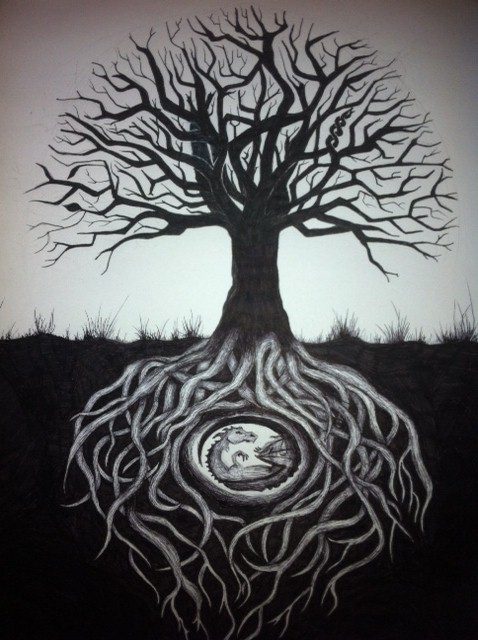
\includegraphics[width=4cm]{pictures/drachenbaum.jpg}
  \end{flushright}
\end{minipage}
\hfill
\end{minipage}
\end{figure}

Im Falle der untersuchten Subglobule, die dem Element Vita zuzuordnen ist, zeichnet sich die Kontaktstelle durch üppige 
Vegetation aus, die trotz des kargen, schieferhaltigen Untergrunds genügend Nahrung findet um sich zu erhalten. Da sie 
sich aufgrund von Dislocationen in den Kraftlinien Condras während der Untersuchungen verschob, konnte die Veränderung 
des Ortes, der innerhalb weniger Tage zur Kontaktstelle wurde, gut beobachtet werden. In einer quantitativen Bestimmung 
der Flora wurde eine Verdreifachung des ursprünglichen Bewuchses und eine Verdoppelung in der Vielfalt der Arten 
festgestellt.

Mit den übernatürlichen Sinnen ist die Kontaktstelle einer Globule nicht leicht zu erfassen, da sie in allen bekannten 
Fällen an starken Kraftlinien oder –knoten liegen. Die Kraftströme überlagern beinahe immer die einfachen Methoden der 
übernatürlichen Sicht, so dass der Forscher auf komplexere Messmethoden angewiesen ist um die Nähe einer Globule zu 
beweisen. Da durch die Verschiebung des Liniennetzes die Astralkarten Condras ohnehin überarbeitet werden müssen, wurde 
eine eher zeitaufwändige Kraftlinienvermessung nach Silbenschwenk durchgeführt. Mittels dieser Ergebnisse war es möglich, 
an verschiedenen, fest definierten Punkten der fraglichen Linie Klicks über eine bestimmte Zeit zu messen und damit die 
Oszillation zwischen den Kompartimenten der Linie zu berechnen.
Stößt man in der normalerweise konstanten Schwingung zwischen zwei Kompartimenten auf eine Fluktuation zwischen 40 und 
150 Klicks pro Pendelschwung, kann man davon ausgehen, eine Kontaktstelle gefunden zu haben. Wichtig ist hierbei, dass 
alle möglichen astralen und elementaren Phänomene geringe Fluktuationen (unter 3 Klicks Differenz pro Pendelschwung) 
hervorrufen, so dass die bloße Anwesenheit eines übernatürlich Begabten schon eine Abweichung produzieren kann. Um 
möglichst genaue Ergebnisse zu erzielen ist es nötig, die Impulse sämtlicher bekannter Faktoren der Messung getrennt und 
abgeschirmt zu bestimmen um dann die Summe der Klicks aller Störfaktoren von den tatsächlich gemessenen abzuziehen. 

Alternativ kann ein erfahrener Begabter, der in der Lage ist, Kraftlinien mit mindestens drei seiner übernatürlichen Sinne 
zu erfassen, sich in die Struktur eines Ortes einklinken und über die Kraftlinien den Zugang zur Globule erspüren. Ob der 
Zugang zum Kraftnetz durch Meditation oder einen physischen Übergang in die Astralebene erfolgt ist hierbei egal: jeder 
Magier oder Elementarist sollte die Methode verwenden, mit der er am Besten vertraut ist. Die häufigsten mit einer 
Kontaktstelle assoziierten Eindrücke sind der Geruch nach Kampher, das Gefühl, gegen den Strich über ein Brennnesselblatt 
zu streichen und der folgende visuelle Eindruck, der wie ein Fortsatz des Kraftlinienbündels wirkt und in Richtung der 
Globule abzweigt:

Bei dieser Methode darf niemals die Gefahr durch ein verunreinigtes oder gar verseuchtes Kraftnetz außer Acht gelassen 
werden. Sind die Bewohner der Globule feindlich gesonnen oder wird das Kraftnetz außerhalb der Globule durch ein 
feindliches Wesen kontrolliert, kann das Einklinken in ein astrales oder elementares Netz einen Angriff provozieren. 

\newpage

\subsection {III: Natur einer Globule}

Kapitel III: Wie man die Natur einer Globule bestimmt

Anhand der makroskopischen Einwirkungen der Globule an der Kontaktstelle kann meist schon eine grobe Aussage über das 
erschaffende Wesen und den Zweck der Globule getroffen werden. Bei elementaren Globulen beobachtet man beispielsweise 
immer einen Einfluss der primären Eigenschaften des entsprechenden Elements, wie Abweichungen im Mikroklima des Ortes oder 
Veränderung in Boden, Flora und Fauna. 

Eine sehr einfache Methode die Natur einer Globule zu erforschen ist es, den Erschaffer derselben zu kontaktieren und sich
mit ihm zu unterhalten. In den meisten Fällen handelt es sich um ein intelligentes Wesen das sich seiner Umgebung bewusst 
ist und sich oft sogar über eine gepflegte Konversation freut. „Wenn man die Konstruktion eines Gebäudes erforschen will, 
ist der Weg über den Erbauer meist der Beste“: dieser Merksatz gilt für Globulen ebenso wie für alles von intelligenten 
Wesen geschaffene. 
Ist es nicht möglich, mit dem Erschaffer der Globule zu kommunizieren, sind umständlichere Methoden vonnöten um Art und 
Nutzen einer Globule herauszufinden. Zunächst sollte man davon absehen, blind in die Globule hineinzustolpern ohne zu 
wissen, was für Bedingungen man vorfindet. Es ist wichtig, sich mit der Struktur der Hülle vertraut macht bevor man 
unkontrolliert Löcher in sie hineinreißt. Erst wenn die Hülle bekannt ist, kann man zunächst unter kontrollierten 
Bedingungen niedere Lebewesen (anfangs Pflanzen, später Tiere) in die Globule transferieren um zumindest eine 
Lebensfeindlichkeit des Globuleninneren auszuschließen. Sind diese beiden Vorraussetzungen – bekannte Hüllenstruktur und 
lebensfreundliche Bedingungen im Inneren-  erfüllt, kann sich auch ein höheres Wesen in die Globule hineinwagen um 
Messungen und Beobachtungen durchzuführen. 

\newpage

\subsection{IV: Ergebnisse}

Kapitel IV: Die Ergebnisse einer Untersuchung 

Die Kontaktstelle 
Aufgrund makroskopischer Beobachtungen (untypischer Pflanzenbewuchs auf sonst kargem Schieferboden, zufälliger direkter 
Kontakt zum erschaffenden Wesen durch bloße Meditation, großes Aufkommen minderer Humus-Elementargeister) konnte die in 
Frage kommende Kraftlinie und die ungefähre Strecke leicht eingegrenzt werden. Die direkte Verbindungslinie zwischen den 
Knoten in Schieferbruch und denen oberhalb von Tharemis wurde als Kontaktlinie ermittelt: der Ort der Messung waren je 800 
Schritt in jede Richtung vom Goldkrug-Dreieck aus. Dieser 1600 Schritt lange Kraftlinienabschnitt wurde in 32 Kompartimente 
aufgeteilt, die einzeln vermessen und verglichen wurden. Mittels einer einfachen Zählung der elementarmagischen Ausschläge 
(Klicks) über eine Zeit von 10 Pendelschwung, die mit einem 1:5-Pendel bestimmt wurde, konnte das Kompartiment, in dem sich 
die Kontaktstelle befindet ermittelt werden.
Als zusätzliche Referenz wurden der Impuls der ersten 8 Klicks und das dominierende Element aller Klicks mittels 
Farbendiagnostik bestimmt. Auffällig waren die zwei Nachbarkompartimente der Kontaktstelle: das dominierende Element war 
in beiden Fällen Cryo, was erstens selten und zweitens für einen Ort in direkter Nachbarschaft zu einer Vita-Globule sehr 
untypisch ist. 


Ein Auszug aus den Rohdaten der Messung:

\begin{table}[htbp]
\begin{center}
\begin{tabular}{|c|c|c|}
\hline
Kompartiment	&dominantes Element	&Impuls	\\
\hline
VI	&18	&90	\\
VII0	&20	&100	\\
VIII	&24	&120	\\
IX	&18	&90	\\
X	&20	&100	\\
XI	&19	&95	\\
XII	&16	&80	\\
XIII	&13	&65	\\
XIV	&39	&195	\\
XV	&15	&75	\\
XVI	&17	&85	\\
XVII	&21	&105	\\
XVIII	&18	&90	\\
XIX	&18	&90	\\
XX	&16	&80	\\
XXI	&20	&100	\\
XXII	&19	&95	\\
XXIII	&17	&85	\\
XXIV	&17	&85	\\
\hline
\end{tabular}
\label{Winkel der hochsymmetrischen Achsen zu (111)}
\end{center}
\end{table}

Die gemessene Kontaktstelle erwies sich als korrekt: es konnte an diesem Ort sehr einfach eine direkte Verbindung zur Hülle 
der Globule hergestellt werden.

\subsubsection{Die Hülle}
Das Studium der Hüllen von mehreren Globulen zeigt, dass eine Barriere aus Nichts, ein beinahe perfektes Vakuum die Globule 
von den Ebenen trennt. Selbst für die meisten Ebenen feste Dimensionen wie Raum oder Zeit sind in diesem Raum nicht 
vorhanden. Es ist für Materie, Zeit, Seele und Energie unmöglich, diese Barriere zu überwinden. Gleichzeitig ist sie von 
beiden Seiten von einem Film oder einer Membran aus sehr schweren Teilchen überzogen, die verhindern, dass der leere Raum 
kollabiert. Die Natur der Teilchen der Innenmembran variiert von Globule zu Globule, während die Außenmembran bei allen 
untersuchten Globulen gleich aufgebaut war. 
Die Untersuchung einer dem Chaosgott Slaneesh zugeordneten, klerikalen Subglobule ergab beispielsweise, dass die 
Innenmembran aus Seelenpartikeln -manchmal auch „Staub“ genannt- bestand, die mittels einer emotionsähnlicher Energie 
vernetzt waren, die leider nicht weiter untersucht werden konnte. 
Der Film auf der inneren Membran der untersuchten Humus-Globule erwies sich als weniger abstrakt: es handelt sich um wahres 
Element der Art Vita. 
Egal welcher Natur die Innenmembran ist, sie erlaubt den Austausch von Materie, Zeit, Seele und Energie zwischen der Globule 
und den anliegenden Ebenen. Mit etwas Krauftaufwand kann selbst ein Fremder, der die Globule weder bewohnt noch sie erschaffen 
hat die Partikel beugen und sie so anordnen, dass sie einen Durchgang bilden und das Ein- oder Austretende vor der Barriere 
aus Nichts schützen. 
Die Außenmembran bestand in allen untersuchten Fällen aus Orichalkum, der perfekten Vereinigung aller sechs Elemente. Da die 
Membranen von Sphärengrenzen oft ebenso aufgebaut sind, liegt es nahe, dass ein Wesen wie ein Humus-Dschinn, der von Natur 
aus nicht in der Lage ist Orichalkum zu erschaffen, eine Sphärengrenze beugt, sie zur Membran seiner Globule formt und die 
Innenseite nach seinen Bedürfnissen auskleidet. Wesen, die nicht einer elementaren Ebene entstammen, sind demnach nicht auf 
eine bereits vorhandene Sphärenmembran angewiesen, da sie –natürlich nur mit erheblichem Aufwand- theoretisch in der Lage 
sind Orichalkum herzustellen.
Versuche ergaben, dass eine kurzlebige und instabile Globule auch mit weniger komplexen Außenhüllen konstruiert werden kann. 
Eine Vernetzung von wahrem Element ergibt beispielsweise eine Hüllmembran, die je nach Güte der Vernetzung einige Stunden 
bis zu mehreren Tagen hält, bevor die Globule kollabiert. Allerdings kann in einer solchen Globule kein komplexer 
Energiekreislauf hergestellt werden ohne die Membran zu zerreißen. Masse und ideelle Faktoren hingegen stellen hierbei kein Problem dar. 

\newpage

\subsubsection{Der Erschaffer}
Es handelt sich um einen alten, benannten Humus-Dschinn, dessen Name vor allem in Dokumenten auftaucht, die den Elfen 
zugeordnet werden. Es ist sehr wahrscheinlich, dass dieser Dschinn von den Elfen seinen heutigen Namen und seine Existenz 
in dieser Ebene erhielt: 

Eru Loa Rava

Vor und während der Zeit der nekanischen Besatzung wurde weder dem Dschinn noch der Subglobule viel Aufmerksamkeit zuteil: 
die Kontaktlinie war zwar schon immer eine recht wichtige Verbindung von Oben nach Unten, zwischen Schieferbruch und 
Tharemis, aber da EruLoaRava kaum Einfluss auf seine Umwelt nahm und selten mit Menschen in Kontakt trat wurde er 
schlichtweg nicht bemerkt. Erst mit der Verschiebung der Kraftlinien am Nachtwall und den daraus folgenden Neuvermessungen 
wurde die Kontaktstelle wieder entdeckt und zunächst nicht als solche erkannt sonder als vernachlässigbare Auffälligkeit 
vermerkt. Durch die Errichtung des Goldkruges in der Mitte dreier sich kreuzender Kraftlinien, zu denen auch die 
Kontaktlinie der Subglobule gehört („Goldkrugdreieck“), kam der Dschinn mit Menschen und schließlich auch mit 
Elementaristen in Kontakt. Die erneute Verschiebung des Netzes im Sturm auf Schieferbruch schob das Dreieck enger um den 
Goldkrug und verdichtete auch die Verbindung der Kontaktlinie zu dem vielgenutzten Knoten im Goldkrugdreieck. 

Die Kontaktaufnahme erwies sich als recht einfach, da EruLoaRava ein neugieriges und geduldiges Wesen ist, mit dem die 
Kommunikation geradezu ein Vergnügen ist. Bisher wurde noch keine physische Manifestation beobachtet. Vielmehr wurde die 
Präsenz eines kollektiven Geistes beobachtet, die in der Lage ist, auch menschliche Körper zu übernehmen. Hierbei geht der 
Dschinn allerdings recht rücksichtsvoll vor: wehrt sich der den Körper bewohnende Geist, zieht er sich sofort zurück. 
Außerdem kann der Autor aus eigener Erfahrung berichten, dass EruLoaRava immer sehr sorgsam mit geborgten Körpern umgeht 
und ihre Strukturen in der Regel intakter zurücklässt als sie es vor der Übernahme waren. Dieses Verhalten konnte auch nur 
dann beobachtet werden, wenn eine größere elementare Störung im Einflussbereich der Globule vorlag. Offensichtlich 
interessiert sich die Entität sehr für das, was in seiner Umgebung vorgeht, greift aber nur dann in der physischen Ebene 
ein, wenn es sein Heim gefährdet sieht und dann auch nur mit Hilfe fremder Körper, nie mit der eigenen physischen 
Anwesenheit. Tut er dies, zeigt er sich allen Phänomenen der physischen Ebene gegenüber sehr wissbegierig und freut sich 
über jede Geschichte, die ihm erzählt wird und jeden sinnlichen Eindruck der ihm gewährt wird. Dieses Verhalten und die 
kollektive Natur der Entität legen nahe, dass es für den Dschinn schwierig ist, eine singuläre Präsenz zu bilden und er 
deshalb nicht ohne weiteres auf der phyischen Ebene erscheinen kann oder will. 

\subsubsection{Das Innere}
Die Bedingungen in der Subglobule erlauben die Existenz von Pflanzen und Lebewesen der physischen Ebene. Allerdings neigen 
die Dinge im Inneren der Subglobule dazu, zu verschmelzen, sich zu vereinen und neue Dinge hervorzubringen, so dass Materie, 
Geist und Seele nur in einem stark beschleunigten, aber dennoch den natürlichen Gesetzen der physischen Ebene gehorchenden
Kreislauf existieren. Ein Wesen mit Bewusstsein kann in dieser Umgebung nicht ohne weiteres seine Identität bewahren und 
läuft Gefahr, sich in diesem Kreislauf zu verlieren. Bereits bei einem kurzen Besuch bemerkt man ein Ziehen in der Struktur, 
dem man sich nur durch absolute Kontrolle der eigenen Physis entziehen kann. Eine ungeübte Person verschmilzt beinahe sofort 
mit der Vegetation der Globule und kann nur mit Gewalt und den daraus resultierenden Strukturschäden wieder aus ihr entfernt werden. 
Diese Eigenschaften machen eine direkte Erforschung des Inneren sehr schwierig, erlauben aber interessante Rückschlüsse auf 
den oder die Bewohner der Globule. So decken sich die in der Subglobule gemachten Erfahrungen mit schriftlichen Berichten, 
in denen die Bedingungen auf der Elementarebene des Humus festgehalten wurden. Lediglich die distinktive Vegetation fehlt 
in den Berichten, in denen eine undefinierbare, ständig die Form wechselnde Masse beschrieben wird anstelle der Ranken, 
Bäume und Sträucher, die in der Subglobule zu erkennen waren. Man kann also einen direkten Vergleich zwischen der 
Subglobule des Dschinns und seiner ursprünglichen Heimat, der Ebene des Humus ziehen. Für einen geübten Elementaristen ist 
es also möglich, in der Subglobule Techniken und Methoden zu erproben, die ihm in der Elementarebene seine Identität 
bewahren könnten. Der physische Übertritt in eine Elementarebene bleibt dennoch ein nahezu wahnsinniges Unterfangen, auch 
wenn die Mechanismen einer solchen Umwelt mit Hilfe der untersuchten Subglobule nun besser bekannt sind. 

\newpage

\subsection{V: Schaffung einer Globule}

Kapitel V: Die Schaffung einer Globule

Mit den erhobenen Daten und den gemachten Erfahrungen verstehen wir nun die Natur von Globulen dergestalt, dass die Idee 
einer menschgeschaffene Globule in greifbare Nähe rückt. 
Die größte Schwierigkeit besteht in der Auswahl einer geeigneten Substanz, mit der eine stabile Hülle geformt werden kann. 
Natürlich ist Orichalkum die beste Wahl, aber seine Herstellung ist äußerst aufwendig und gefährlich, weshalb in einer 
Demonstration davon abgesehen wird, die Außenmembran aus Orichalkum zu fertigen. Für ein konkretes Projekt allerdings ist 
es unabdinglich, das kostbare Material zu nutzen, da eine Globule nur mit einer Hüllmembran aus Orichalkum dauerhaft und 
stabil ist. 

Es muss also eine Alternative zu Orichalkum gefunden werden. Diese Substanz muss großen Energien widerstehen können und 
darf weder starr noch weich sein. Sie darf durch Einflüsse von Kräften, Ideen oder Emotionen nicht veränderlich sein und 
muss gleichzeitig genügend physische Präsenz aufweisen um eine Barriere für Materie und materielle Energie darzustellen. 
Nach dem Vorbild der Humus-Globule im Goldkrugdreieck wurden Versuche mit wahrem Element Humus gemacht, die akzeptable 
Ergebnisse lieferten. Je reiner eine Substanz ist, desto starrer ist auch ihre Struktur, weshalb selbst die Verwendung von 
wahrem Element keine perfekte Lösung darstellt. Da Humus allerdings ein flexibles Element ist, funktioniert es als 
Schutzschicht der Hülle einer Globule, auch wenn vernetzte Strukturen mehrerer unterschiedlicher Komponenten 
(beispielsweise Verbindungen aus physischen und ideellen Partikeln) eine elegantere und vermutlich auch stabilere Lösung 
wären. Da wir vorerst nur beweisen möchten, dass eine Globule auch von Menschen geschaffen werden kann, nehmen wir mit der 
etwas plumperen, aber dafür weniger aufwändigeren Lösung vorlieb und nutzen wahres Element Vita um die Hülle abzuschirmen.

Um die Partikel in der gewünschten Form anzuordnen ohne dass sie sofort in die Umgebung diffundieren wird eine stützende 
Sphäre benötigt. Ob die Sphäre materiell oder energetisch aufgebaut ist spielt keine Rolle, solange sie leicht aus der 
fertigen Struktur entfernt werden kann. Hat man also eine Schutzhülle aus wahrem Element Vita um die Sphäre konstruiert, 
wird jegliche Materie und Energie aus dem Zwischenraum entfernt. Hierfür wird bei der Konstruktion der Schutzhülle eine Art 
Reuse eingebaut, die es erlaubt, Materie und Energie nach außen abzuführen und den Rückstrom gleichzeitig aufzuhalten. 
Schließt man die Austrittsstelle an ein System mit einer Energie- und Masseninsuffizienz an, reicht ein einziger kräftiger 
Impuls um den gesamten Inhalt der Hülle in dieses Hilfssystem abzuleiten.
Um eine perfekte Hülle zu schaffen ist es nötig, neben Energie und Masse auch Zeit und Seele aus dem Zwischenraum zu 
entfernen. Große Teile dieser abstrakten Substanzen heften sich zwar an die ausströmenden physischen Substanzen, aber eine 
komplette Leere zu schaffen ist einem Menschen mit seinen eigenen Mitteln nicht möglich. Hierbei machen wir uns eine 
Eigenart der Elemente Mitrasperas zunutze, einem Kontinent auf dem „die Leere“ ein Element darstellt, dessen Essenz von 
entsprechend sensitiven Wesen erfasst und genutzt werden kann. Ein winziger Teil der Essenz einer Viinshar, eingebaut in 
das Hilfssystem genügt, um auch die abstrakten und schwer greifbaren Energien abzuleiten. Um sicher mit dieser 
lebensfeindlichen Essenz umgehen zu können, ist es nötig diese stark zu verunreinigen. Dies schwächt den Effekt des 
Hilfssystems zwar ab,  genügt aber um eine stabile, undurchdringbare Hülle für eine kleine Globule zu erhalten. 

Es ist ratsam, den Inhalt der Globule vor der Konstruktion der Hülle zu implementieren, da es sehr kraftaufwändig ist, 
wahres Element zu beugen um einen stabilen Durchgang durch die Hülle zu erzeugen. Alternativ ist es möglich, die komplette 
Globule zu dehnen, die Hülle  kontrolliert kollabieren zu lassen und Dinge ähnlich einer Amöbe in die Globule aufzunehmen.
Danach muss der Innenraum der Hülle allerdings erneut entleert werden, außerdem ist eine kompakte, potente Kraftquelle 
nötig um die Globule gleichmäßig auszudehnen. 

Eine leere Globule zieht sich nach wenigen Stunden zusammen und implodiert spätestens nach zwei Tagen. Um eine Globule mit 
einer längeren Lebensdauer zu erschaffen ist es nötig, im Inneren einen stabilen Kreislauf zu etablieren. Es ist nicht 
zwingend notwendig, hierfür ein System mit einander ergänzenden Lebewesen zu konstruieren: ein simples abgeschlossenes 
System mit mindestens zwei Elementen genügt. Dieses System muss so lange funktionstüchtig sein, bis sich eine Kontaktstelle 
ausgebildet hat. Bei sämtlichen Versuchen erfolgte dies nach wenigen Stunden selbstständig und ohne Einfluss von Außen. 
Sobald die Kontaktstelle erkennbar ist, kann das System auch von außerhalb der Globule beeinflusst und der Kreislauf auch 
künstlich aufrecht erhalten werden. Es ist möglich, über die Kontaktstelle Kraft zuzufügen oder abzuziehen, Materie 
hingegen muss über einen aufwändigen Durchbruch in der Hülle hinzugefügt werden.

Eine solcherart gefertigte und stabilisierte Globule besitzt die gleichen Eigenschaften wie die in vivo beobachteten 
Subglobulen. In Größe und Komplexität des Innenlebens ist sie noch unterlegen, doch diese Faktoren sind lediglich eine 
Frage der eingesetzten Kraft. 

\newpage

\section{Narrativum}

%\yinipar{M}
M"ogen sie mir verzeihen das ich in dieser Vorlesung ein wenig die ausgetretenen Fade der Naturbeschreibenden Wissenschaften 
verlasse und auf die Geisteswissenschaften der Philosophia und der Erkenntnistheorie zur"uckgreifen werde.
Narrativum ist keine tats"achlich existente Substanz, Mittel oder Energie vielmehr ein Hilfskonstrukt f"ur unseren 
Geist mit dem sich allerdings Tatsachen und Sachverhalte erkl"aren la"
ssen und beweisen lassen. Narrativum befindet sich in allem und jedem, jedes noch so mikroskopische Objekt besitzt einen gewissen 
Wert an Narrativum und dem Prinzip der Superposition folgend besitzt jedes makroskopische Objekt, einen Narrativumswert, der der 
Summer der Werte seiner Einzelteile entspricht.
Narrativum ist ein Wert f"ur die Wichtigkeit eines Objektes im Raum Zeit Gef"uge. Das Wort selbst kommt von dem Verb narrare, 
erz"ahlen. Es ist ergo ein Ma"s f"ur die Tatsache ob es sich lohnt dar"uber zu erz"ahlen. Narrativum hat keine konkrete Ma"seinheit 
bzw. Dimension sondern wird bestenfalls mit Begriffen wie „viel“, „wenig“ oder „fast gar nicht“ gemessen auch sind Vergleiche mit 
anderen Objekten und deren Narrativumsgehalt sehr schwierig bis gar unm"oglich und s"amtliche Einsch"atzungen absolut subjektiver Natur.
Ist diese vage Definition erst einmal verstanden ist das Arbeiten mit diesen Werten recht einfach man mu"s sich lediglich von der 
Vorstellung verabschieden objektive und absolute Werte und Aussagen zu erhalten, in dieser Betrachtungsweise ist alles relativ.
Einige Bespiele zum Verdeutlichen:
Ein Stein der am Wegesrand liegt hat recht wenig Narrativum, denn keiner wird sich jemals an ihn erinnern und "uber ihr Erz"ahlen. 
Wenn nun allerdings ein Wagen "uber ihn f"ahrt und sich die Achse bricht, dann hat der Stein eine recht gro"se Menge an Narrativum, 
der H"andler wird sich nun die ganze Woche dar"uber "argern. Ist der Stein der Grund das die Achse bricht w"ahrend der H"andlern 
von Dieben auf der Flucht ist und die Diebe k"onnen ihn nur wegen des Steines stellen und seine ganze Ladung Rauben, dann wird sich 
der H"andler ein Leben lang "uber diesen Stein "argern und der Stein hat sehr viel Narrativum. W"urden die Diebe den H"andler t"oten 
w"urde er sich nicht "uber den Stein "argern, da er tot ist und den R"aubern w"ar es egal warum die Achse brach, also w"urde keiner 
"uber den Stein erz"ahlen, aber dennoch h"atte er einen sehr gro"sen Narrativumsgehalt weil er das Potential zu einer gro"sen Geschichte 
h"atte, zumindest aus unserer Sicht. Also noch mal zusammengefasst letzterer Stein h"atte aus 
Sicht der R"auber und des H"andlers wenig aus unserer aber recht viel Narrativumsgehalt (da wir ja davon wissen das der Stein Schuld 
war), soviel zur Objektivit"at.
Ein Objekt hat schon einen objektiven Gehalt an Narrativum, doch wir verm"ogen ich nicht zu messen, da wir selbst subjektiv sind. 
Kaiser Jeldrik hat einen Immensen Anteil an Narrativum jeder erz"ahlt von ihm, ja wir benannten sogar unsere Zeitrechnung nach ihm, 
doch in anderen L"andern ist dieser Engonische Nationalheld recht wenig bis gar nicht bekannt, das schafft einen weiten Bogen an 
Variationen die Objektiv zu einem Mittelwert verarbeitet werden m"ussten, doch da wir nicht wissen wie viele Menschen es in den 
Dimensionen gibt geschweige denn Tiere und Gegenst"ande (die ja auch durch Jeldriks Pr"asenz beeinflu"st worden sein k"onnten) kann 
unsere Sch"atzung nur subjektiv bleiben.\\

Wozu brauche ich nun einen Wert f"ur Narrativum, wenn er so unheimlich ungenau ist wird sich der geneigte Leser fragen, die Beispiele 
daf"ur sind recht zahlreich aber ebenfalls recht ungenau (dies scheint sehr in der Natur der Wahrscheinlichkeits und Sph"arenereignisse 
zu liegen). Zum Beispiel die Wahrsagerei (nun sp"atestens werden viele Kollegen wieder mit den Augen rollen) und Hellseherei wird von 
gro"sen Ereignissen, sprich Ereignissen mit viel Narrativumsgehalt angezogen. Epische Schlachten und Schicksale von ber"uhmten Kriegern 
ziehen die Aufmerksamkeit der Zukunftsdeuter auf sich, so da"s man in unserer hermetischen Terminologie davon sprechen kann das das 
Narrativum die Hellseherei leitet und bestimmt was gesehen wird.
Die Fachgemeinde der Magier und Magierinnen wird aber ein konkreteres Beispiel fordern und ich werde es bringen, obwohl dies sehr kompliziert 
ist und einen Gro"steil der mir zur Verf"ugung stehenden Zeit beanspruchen wird, n"amlich die Zeitreisen.
Zeitreisen existieren, davon kann man nach Existenz des 5. Zirkel Zaubers „Zeitkontrolle“ als allgemein bekannte Tatsache ausgehen. 
Weiterhin ist es als gesicherte Tatsache anzusehen das die Zeit nicht linear verl"auft sondern Wirbel H"ugel und ebene Fl"achen aufweist.
„Die Zeit vergeht wie im Flug“ sagt man wenn einem ein langer Spaziergang mit seiner Liebsten im Park gut gef"allt oder „die Zeit stand 
still“ als sie sich sahen. Ebendies wird durch das Narrativum beeinflusst, an schlimme Ereignisse (gro"se Schlachten, viel Narrativum) 
erinnert man sich stark, „als w"are es gestern gewesen“ w"ahrend man die 5 Tage die man im Hafen auf ein Schiff wartet zwar in dem Moment 
als Lang empfindet, die aber nachher, da recht ereignislos als minderwertig und nicht erw"ahnenswert im Ged"achtnis erinnert werden. Diese 
Beispiele sollen aber nun keinesfalls einen linearen Zusammenhang zwischen Narrativumsmenge und Schnelligkeit der Zeit implizieren sondern 
vielmehr einen sehr viel komplexeren Zusammenhang.
Der weitaus weniger bekannte Zauber Cronoclassis erlaubt es einen Gegenstand aus der Vergangenheit in die Gegenwart zu bringen z.B. Kaiser 
Jeldriks Schwert oder Hargarts Glocke oder dergleichen, dabei kommt es sehr auf eine besondere Eigenschaft des Narrativums an n"amlich der 
Zeit/Raum Konsistenz. Der Narrativumsgehalt eines Gegenstandes ist Ort und Zeit unabh"angig uns bleibt immer gleich egal wann man ihn 
betrachtet. Ein neu geborenes Kind in einem kleinen Bauerndorf in Andarra w"are ja eigentlich nicht besonderes, aber der Narrativumsgehalt, 
dieses Kindes ist "uber alle Ma"sen hoch, so da"s jemand der zu diesem Zeitpunkt den Narrativumsgehalt feststellen k"onnte schon sagen kann 
das dieses Kind zum Andarrianischen Feldherrn und zuk"unftigen Herrscher "uber alle Engonier wird. Angemerkt sei hier auch der Selbstschutz 
des Narrativums vor Ver"anderung, denn sollte besagter Beobachter nun das Kind t"oten weil es ein so hohes Narrativum hat w"urde es nicht 
ber"uhmt werden und demzufolge ein geringeres 
Narrativum haben, dann aber h"atte der Beobachter das Kind nicht ge"otet, weil unwichtig, Paradoxon. Das Narrativum kennt, da es au"serhalb 
von Raum und Zeit steht, die komplette Geschichte eines Objektes und sch"atzt sich dementsprechend ein und bestimmt seine Gr"o"se, auf unser 
Beispiel bezogen hei"st das, da"s das Narrativum schon vorher w"usste ob das Kind get"otet wird oder nicht.
Um auf den Cronokla"sis zur"uckzukommen hei"st dies das die magische Energie die ben"otigt wird um ein Objekt in unsere Zeitepoche zu versetzen 
direkt proportional zum Gehalt an Narrativum dieses Objektes ist. Ein Stein aus dem Wald fast ohne Narrativum bedarf fast keiner Energie 
um ihn herzuholen, besagtes Schwert des Kaisers aber sehr wohl.
Dies verdeutlicht einen weiteren immensen Nutzen, den wir aus der Einf"uhrung von Narrativum ziehen k"onnen. Mit Hilfe des Gehaltes an 
Narrativum k"onnen wir die Auswirkungen von Zeitreisen auf das Raum/Zeit Gef"uge messen, verstehen und ihm vorbeugen. Sehen wir nun einmal 
von den sehr komplizierten Paradoxen ab k"onnen Zeitreisende durch ihre Handlungen in der Vergangenheit die Zukunft ver"andern. Eine 
g"angige Warnung in Verbindung mit Zeitreisen ist das auch die kleinste Ver"anderung in der Vergangenheit immense Auswirkungen in der Zukunft 
haben kann, man bedient sich oft der Analogie einen Stein in einen See zu werfen und die Wellen (wie durch die Zeit) sich immer weiter 
ausbreiten zu sehen. Dies ist mitnichten so einfach und pauschal zu sagen und soll an dieser Stelle durch Folgende Erklärung ersetzt werden, 
bis ich das Thema in einer zuk"unftigen Vorlesung noch einmal aufgreifen werde. Ein Zeitreisender ver"andert die Zukunft in dem Ma"se indem 
er Kontakt zu Narrativum in der fremden Zeitepoche hat 
und Objekte die hohes Narrativum tragen ver"andert. Will hei"sen ein Zeitreisender kann Gegenst"ande mit geringem Narrativum ver"andern soviel 
er Lust hat ohne das dies gro"se Auswirkungen (oder Irgendwelche) auf die Zukunft haben wird, sollte er aber Objekte mit hohem Narrativum aus 
ihrem Zeitrahmen rei"sen, wird dies besagten Domino bzw. Wellenkreis Effekt haben. Um sichere Zeitreisen zu erm"oglichen w"are es also recht 
angebracht einen „Narrativumsmesser“ zu erfinden der einen Zeitreisenden sicher durch die Zeit geleiten kann.\\

Die Raum/Zeit Konsistenz erm"oglicht ein weiteres bedeutendes Gedankenexperiment, das „Diktatorische Schicksal“. Wir Menschen sehen unsere 
Zukunft oft gerne als Unbestimmt, das wir selbst unser Gl"uckes Schmied sind und das nichts in unserem Leben vorbestimmt ist. Andererseits 
sehnen sich viele oft nach einem vorbestimmten Leben einem Schicksal einem Pfad der ihnen vorbestimmt ist, so das sie an ihren Schicksalsschlägen 
nicht selbst Schuld sind sondern es der vorbestimmten Zukunft in die Schuhe schieben k"onnen.
F"ur Vertreter beider Richtungen habe ich eine gute Nachricht, denn mit Hilfe des Narrativums kann man diese Frage entg"ultig l"osen.
Erinnern wir uns an die Eigenschaften des Narrativums, das Narrativum ist Raum/Zeit Konsistent also wei"s das Narrativum bereits im Voraus welche 
Zukunft dem Objekt bestimmt ist, oder besser ausgedr"uckt nicht im Voraus, denn das Narrativum steht au"serhalb der Zeit, es gibt f"ur das 
Narrativum kein „Vorher“. Das hei"st also das ein kleines Kind in einem Bauernhof in Andarra geboren mit einem immensen Gehalt an Narrativum 
kein Bauer werden und ein bescheidenes Leben f"uhren wird, egal f"ur was es sich entscheidet, das Schicksal wird zuschlagen und ihn auf einen 
Weg zur Ber"uhmtheit f"uhren.
Nun kommt die gute Nachricht f"ur Diejenigen die die Theorie der frei w"ahlbaren Zukunft bevorzugen, einfach aus der Tatsache, das wir Narrativum 
nicht genau messen k"onnen. Wir k"onnen Narrativum nicht genau messen nicht weil wir nicht die Ger"ate und Methoden dazu haben, sondern weil es 
schlicht und einfach nicht perfekt zu bestimmen ist.\
Also kann man zusammenfassend sagen, da"s das Schicksal von jedem von uns zwar festgeschrieben ist wir es aber unter keinen Umst"anden messen 
oder bestimmen k"onnen.\\

Dieses Gedankenexperiment "uber das Diktatorische Schicksal liefert uns zusammen mit der Unbestimmtheit des Narrativumswertes das wir von nun 
an Unsch"arferelation nennen werden eine wissenschaftlich fundierte Erklärung zur Hell- und Wahrsagerei. Der Grund warum Hell- und Wahrsagerei 
in der Fachwelt einen so schlechten Stand haben ist ihre Ungenauigkeit. „Wenn sie die Zukunft vorhersagen k"onnen wieso kleiden sie sich dann 
in nebul"ose Phrasen und Metaphern, die mannigfaltige Interpretationen erlauben“ h"ore ich so manche Magi und Magae sprechen. Manche sehr 
akademische Magier und Magierinnen gehen sogar so weit zu behaupten, Wahrsagerei w"are ganz und gar unm"oglich und die Ereignisse w"urden nur 
manchmal eintreffen, weil die Voraussagen so wage formuliert sind das sie sich zuf"allig auf ein Ereignis beziehen. \
Mit dem nun gelernten k"onnen wir diesen Sachverhalt aber nun ebenfalls kl"aren. Wahrsagerei, eine Kunst von der ich selbst nur die rudiment"arsten 
Kenntnisse aus meiner Grundausbildung besitze, ist die Kunst oder Methodik zu beschreiben und zu messen, was nicht exakt beschrieben oder gemessen 
werden kann. Wie eben bereits beschrieben steht die Wahrsagerei in direkter Beziehung zum Gehalt des Narrativums in einer bestimmten Substanz/Objekt, 
doch aufgrund der Unsch"arferelation kann man diesen konkreten Wert des Narrativums nicht messen, Also mu"s ein unbestimmter Wert gemessen, 
oder besser gesagt etwas "uber ihn ausgesagt werden und daraus entstehen die nebul"osen und zweideutigen Phrasen auch bei den seri"osesten 
Wahrsagern und Wahrsagerinnen. 
Ein Zahlenbeispiel verdeutlicht dies: Angenommen das Narrativum h"atte einen Wert im abgeschlossenen Intervall von 8 bis 12 irgendeine der Zahlen 
8,910,11 oder 12, eine bestimmte, die sich nicht "andert, aber die keiner kennt. Nun müsste man dieses Intervall messen und wie wir wissen 
hat jede Messung eine Ungenauigkeit. Sagen wir ein guter Wahrsager kann mit einer Genauigkeit von +- 1 wahrsagen und ein schlechter Wahrsager 
mit einer Genauigkeit von +-3. Also w"urde der gute Wahrsager ein Intervall von 7 bis 13 und der schlechte ein Intervall von 5 bis 15 angeben, 
also beides sehr vage Au"sagen, die allerdings beide mit absoluter Sicherheit zutreffen w"urden. Beide wollen nun ihr Ergebnis konkretisieren 
um in der magischen Fachwelt Anerkennung zu erhalten und beschr"anken ihr Intervall auf drei bzw. f"unf Ergebnisse jeweils am oberen Ende ihres 
Spektrums. Nun hat der gute ein Intervall von 11 bis 13 und der schlechte ein Intervall von 11 bis 15, also der gute sich auf einige Metaphern 
beschr"ankt, w"ahrend 
der schlechte noch recht viele nebul"ose Beschreibungen verwendet. Wir wissen das der Wert des Narrativums irgendwo zwischen 8 und 12 (inklusive) 
zu finden ist, also eine Chance von 20\% f"ur die 8: 20\% f"ur die 9 usw. besteht. Im Intervall der Wahrsager liegen nun die Werte 11 und 12, die 
je eine Wahrscheinlichkeit von 20\% also zusammen 40\% haben. Das hei"st, daß der gute Wahrsager mit seiner recht konkreten Vorhersage eine Chance 
von 40\% hat das Richtige vorhergesagt zu haben und der Schlechte mit seiner recht nebul"osen auch nur eine Wahrscheinlichkeit von 40\% hat. Hat 
der gute Wahrsager nun Gl"uck wird die Fachwelt erstaunt aufhorchen und auf reproduzierbare Ereignisse warten um die Daten zu verifizieren, hat 
er Pech und die 60\% Chance schl"agt zu werden ihn wieder nur alle auslachen und sagen „das h"atten wir ihnen vorher sagen k"onnen“. Der schlechte 
Wahrsager hat in jedem Fall verloren, denn trifft sein Ereignis ein (40\%) dann werden alle sagen „na deine Vorhersage war so ungenau wenn Ereignisse 
13, 14, 15 eingetreten w"aren h"attest du ja auch recht gehabt, obwohl sie nicht eingetreten sind bzw. h"atten k"onnen“ und wenn er falsch liegt 
w"are das f"ur die Wissenschaftler zu erwarten gewesen. Im besten Fall, also das der Gute Recht hatte (was nur bei 4 aus 10 Versuchen der Fall ist) 
hatte die Fachwelt auf reproduzierbare Ergebnisse gewartet (wie man es immer bei Experimenten macht, Ein Experiment mu"s bei gleicher Durchf"uhrung 
immer wieder zu dem selben Ergebnis kommen um etwas empirisch zu Beweisen) doch das n"achste Experiment w"urde wieder nur zu 40\% klappen, und 
irgendwann wird der gute Wahrsager auch Pech haben und seine Vorhersage trifft nicht zu (was bei den Prozentsatz eigentlich die Regel sein sollte), 
dann wird sich die Fachwelt auf ihn st"urzen und seine Theorie und Me"smethoden f"ur unbrauchbar erkl"aren und wieder behaupten Wahrsagerei w"are Unm"oglich. 
Also zusammengefa"st: Egal wie gut der Wahrsager ist, er wird aufgrund der Struktur des Narrativums nie eine Wissenschaftlich Hieb und Stichfeste 
Au"sage treffen k"onnen. An dieser Stelle sei dann noch angemerkt das wenn der schlechte seine Au"sage so konkretisiert h"atte wie der Gute also auf 
einen Intervall von 13 bis 15 er gar keine Chance gehabt h"atte das sein vorhergesagtes Ereignis eintrifft, und abgesehen davon gibt es in dieser 
Zunft auch noch jede Menge Hochstapler, die gar nichts vern"unftig vorhersagen k"onnen und somit diese Zunft noch tiefer in Diskredit bringen 
als die sowieso schon der Fall ist.\\

Eine ausf"uhrliche Erkl"arung zur Unsch"arferelation bin ich ihnen bis jetzt schuldig geblieben und habe sie lediglich als gegeben vorausgesetzt um 
andere Sachverhalte zu beweisen, dieses Defizit werde ich nun nachholen.
Pauschal lässt sich sagen je mehr Narrativum ein Gegenstand hat, desto schwerer ist seine Menge zu bestimmen, beziehungsweise der Umkehrschlu"s, je weniger 
Narrativum ein Gegenstand hat desto genauer kann man dessen exakten Wert eingrenzen. Dies lässt sich durch folgende Formel leicht ausdr"ucken  
$N * \Delta N = h$ . N  ist der Wert den das Narrativum annimmt,  delta N  das Intervall in dem sich der Wert des Narrativums befindet und h ist eine einfache 
Hilfskonstante, daher h, die recht unwichtig ist und auf die ich hier nicht n"aher eingehen werde. Einige Beispiel um das zu verdeutlichen ein einfacher 
Stein irgendwann irgendwo im Wald der nichts besonderes erleben wird hat einen sehr geringen Anteil an Narrativum keiner nichts und niemand interessiert 
sich f"ur ihn, er ist lokal und global vollkommen unwichtig. Daraus folgt er hat sehr wenig Narrativum das sehr genau den Wert sehr wenig hat. Auf 
der anderen Seiten haben wir Kaiser Jeldrik, der von immenser Bedeutung f"ur das Engonische Volk ist, jeder kennt ihn 
und jeder erz"ahlt sich von seinen Ruhmestaten, er hat einen sehr hohen Wert an Narrativum ohne Zweifel. Doch au"serhalb von Engonien ist er nur m"a"sig 
bekannt und in weit entfernten L"andern und fremden Dimensionen vielleicht gar nicht, was f"ur sich alleine gesehen einen geringen Wert an Narrativum andeuten 
w"urde. Also ist er Lokal von Bedeutung und hat sehr viel Narrativum aber da Narrativum Raum/Zeit Konsistent ist müssen wir einen globalen Wert angeben 
und da wir nicht wissen wie gro"s „alles“ ist ist dies unm"oglich. Daraus folgt das Kaiser Jeldriks immenser Wert an Narrativum nur sehr sehr grob 
angegeben werden kann.
Weder die St"arke des Narrativums noch die Abweichung vom Exakten Wert kann Null betragen, denn h ist eine positive Zahl ungleich Null. Das hei"st es 
gibt kein Objekt was kein Narrativum enth"alt, auch der unwichtigste Stein ist ein ganz, ganz, ganz klein wenig wichtig, irgendwann und es gibt kein Objekt, 
keinen Gegenstand dessen Wert an Narrativum absolut genau gemessen werden kann, es gibt immer einen kleinen Fehler und sei er noch so klein.

\newpage

Nun noch ein kleiner Ausflug in die fundamental Elementartheorie und dann n"ahert sich diese Vorlesung auch schon dem Ende. Jedes Objekt enth"alt f"ur sich 
Narrativum und sei das Objekt auch noch so klein. Spaltet man ein Holzscheit in zwei Teile enth"alt jedes Teil wiederum Narrativum spaltet man nun eins der 
Teile, erleben wir wiederum das gleiche, diesen Proze"s setzen wir weiter fort und spalten die immer eins der Teile bis das Holzscheit so klein ist, daß 
man es nicht mehr spalten kann. Nun befinden wir uns auf der Elementarebene, jedes Objekt und jedes Wesen besteht aus den fundamentalsten Bausteinen des 
Seins, den Elementen Feuer, Wasser, Erde, Luft. Sie sind die unteilbar kleinsten Teilchen aus denen alles besteht. Das hei"st jedes Element hat einen 
eigenen Wert an Narrativum und sie kombinieren all ihre Narrativumswerte um dem Holzscheit, das sie bilden einen festen Wert an Narrativum zu geben und 
alle Holzscheite kombinieren wiederum ihre Werte um dem Lagerfeuer das aus ihnen besteht einen festen 
Narrativumswert zuzuschreiben. Dieses Prinzip nennt man Superposition, alles steht mit allem in Wechselwirkung und bedingt sich untereinander. So werden alle 
mikroskopischen bis hin zu allen makroskopischen Dingen, Objekten, Subjekten, Wesen und was man sich sonst noch so alles vorstellen kann mit einem 
einzigartigen Wert ausgestatten, der ihre komplette Existenz bestimmen wird, den nichts und niemand aber so recht fassen kann.\\

Ich hoffe ich habe ihnen mit dieser Vorlesung einige neue Blickwinkel aufgezeigt und M"oglichkeiten in die Hand gegeben ihre Erkenntnis der Erde des Himmels 
und dem ganzen Rest ein wenig zu erweitern. Querverweise und meine anderen Vorlesungen finden sie wie "ublich in der Bibliothek der Akademie Ayd Owl in Engonien.
\vspace{10mm}
Mit freundlichen Gr"u"sen\
Florian Phelleas Ph"onixflug, Bund zu Ayd Owl\
im Jahre 254 nach Jeldrik oder 1502 der alten Zeitrechnung\

\newpage

\section{Transdimensionale Dislocation}

%\yinipar{W}
Wir beginnen die transdimensionale Dislocation mit einer Abhandlung "uber Deterministisches Schicksal und Chaos. Was unsere eigene Zukunft anbelangt sind wir Menschen 
oft zweierlei Meinung und das oft zur selben Zeit. Zum einen w"unschen wir uns unser Schicksal selbst in die Hand nehmen zu k"onnen und unser Gl"uckes eigener 
Schmied zu sein zum anderen sehnen wir uns nach Stabilit"at und der Sicherheit eines vorbestimmten Lebens.\\

Nun zu ergr"unden wann die Zukunft vorherbestimmt ist und wann nicht ist Subjekt dieser Vorlesung. Der Sinn dieser Fragestellung ist an dieser Stelle allerdings weder 
die Zukunft vorherzusagen noch theologische Fragen aufzuwerfen, sondern lediglich eine Vorarbeit f"ur Zeitreisen zu leisten. An dieser Stelle m"ochte ich ebenfalls 
noch einmal ausdr"ucklich darauf hinweisen, da"s der Begriff Chaos, den ich im Zusammenhang mit dieser Vorlesung gebrauchen werde lediglich eine gro"se Unordnung 
beschreibt und in keinerlei Zusammenhang mit G"ottergestalten oder zurecht verbotenen Spielarten der Magie steht.\\

Wie wir aus grundlegenden Kenntnissen der Dimensionstheorie wissen gibt es viele, wenn nicht gar unendlich viele Dimensionen die alle mit der Dimension der Zeit verkn"upft 
sein k"onnen. Die Zeit messen wir durch einen periodischen, sich immer wiederholenden Vorgang, der seine Periode im zu messenden Zeitraum nicht "andert. Das bedeutet, da"s 
wir die Zeit durch eine einzelne Zahl beschreiben k"onnen. Da wir allerdings nicht wissen ob die Zeit einen Anfang oder ein Ende hat, zumindest nicht innerhalb dieser 
Vorlesung, müssen wir einen beliebigen Punkt als Fixpunkt erw"ahlen und von dort aus sowohl vorw"arts, als auch r"uckw"arts z"ahlen. In der Praxis ist dies die 
Thronbesteigung Kaiser Jeldriks, seit der nun 255 Jahre vergangen sind, respektive die alte Zeitrechnung, nach der wir das Jahr 1503 schreiben. Diese Zahl ist eine einzige 
Gr"o"se, weswegen der Raum der Zeit auch nur eine einzige Dimension besitzt. Soweit h"ort sich die Theorie recht einfach an, allerdings sei zu bedenken, da"s die Zeit nicht 
linear 
ist und unter anderem als imagin"ar aufgefa"st werden kann, was allerdings ebenfalls nicht Teil dieser Vorlesung sein soll und bitte an anderer Stelle gekl"art wird.\\

Zu jedem dieser Zeiten kann ein Ereignis in den anderen Dimensionen eintreten, d.h. es existiert eine eindeutige Abbildung von einem oder mehreren Punkten im Zeitraum in 
den der anderen R"aume mit deren Dimensionen und wieder zur"uck. Zum Beispiel trinke ich Tee heute, morgen und "ubermorgen, damit w"aren einem Ereignis drei Punkte auf 
der Zeitschiene zugeordnet. Dies erlaubt nat"urlich keine Au"sage "uber die Vollst"andigkeit, es ist ja nicht dar"uber bekannt ob ich gestern auch Tee getrunken habe.
Um uns in unserer Fragestellung, die uns am Anfang besch"aftige weiter zu bringen müssen wir uns fragen inwieweit ein Ereignis in der Zukunft feststeht, also ob ich 
morgen wirklich Tee trinken werde zum Beispiel. Dabei stehen wir vor einem gro"sen Problem, denn das ich morgen Tee trinken werde wird subjektiv von immens vielen Faktoren 
bedingt. Der Vorsatz morgen Tee zu trinken reicht ja nicht aus es tats"achlich war werden zu lassen, ich k"onnte ja zum Beispiel morgen keine Teebl"atter finden, oder meine 
Teekanne k"onnte zerst"ort werden oder ich k"onnte durch noch unangenehmere Gr"unde daran gehindert werden.
Mit anderen Worten es gibt immens viele Ver"anderungen von meiner Planung die eintreten k"onnen. Die Anzahl dieser Ver"anderungen sprich die Abweichung von meinem geplanten 
Weg gebe ich mit exp($\Lambda$) an also einer Exponentiellen Steigerung.
Das Verfahren das ich nun beschreiben werde wird es uns erm"oglichen Ereignisse zu finden, f"ur die sich die Zukunft vorhersagen lässt und wir werden lernen sie von 
denjenigen zu unterscheiden f"ur die uns dies, im Rahmen der f"ur die Vorlesung zur Verf"ugung stehenden Mittel, nicht m"oglich ist, dieses Verfahren werde ich Ph"onixflug 
Dimensionsweg Verfahren nennen.\\

Zuallererst betrachten wir eine Abbildung aller Dimensionen in den Phasenraum. Dadurch erhalten wir einen 2 mal f mal n dimensionalen Phasenraum mit f gleich der Anzahl 
der Freiheitsgrade in den betreffenden Unterr"aumen und n gleich der Anzahl der Unterr"aume, sprich Nebenwelten, Paralleldimensionen und so weiter. Dies ist nat"urlich eine 
viel zu gro"se Menge ist, als da"s sie unser Geist fassen k"onnte, aber das braucht er ja auch nicht, denn nun bedienen wir uns der Poincaré Phasenraumschnitte und zerlegen 
den Phasenraum in jeweils zweidimensionale Unterr"aume. Das geschieht einfach in dem wir alle Dimensionen bis auf zwei negieren, vergleichbar mit einem Querschnitt durch 
eine Torte. Diese Phasenraumschnitte sind f"ur uns ohne weitere Probleme zu betrachten, da sie z.B. auf einem Pergament simpelst dargestellt werden k"onnen.
Nun betrachten wir die Pr"asenz eines Ereignisses, dieses hinterlässt im Phasenraum eine Trajektorie, also die Punkte, die es auf andere Abbildet. Da die Poincaré Schnitte 
lediglich zweidimensional sind betrachten wir von der vieldimensionalen Trajektorie nur die Durchsto"spunkte. Diese k"onnen nun im Phasenraumschnitt entweder als 
zusammenh"angende Figuren oder chaotisch wild verstreute Punkte auftauchen. Zusammenh"angende Punkte implizieren einen Zusammenhang zwischen den einzelnen Teilereignissen, 
sind also vorhersagbar, w"ahrend wild verstreute Punkte wie ich oben bereits angedeutet habe sich absolut chaotisch, also unvorhersagbar verhalten. Wie wir an den ersten 
Experimenten in dieser Hinsicht gesehen haben stellen die verstreuten Teilereignisse die Regel und die Figuren eher die Ausnahme dar, daher bezeichnen wir die Figuren, 
zumeist Ellipsen, als Inseln der Stabilit"at und die sie umgebenden verstreuten Punkte als Meer des Chaos.
Der Praktische Nutzen liegt nun darin, das die Teilereignisse auf den Inseln der Stabilit"at in einer Beziehung zu den anderen stabilen Teilereignissen stehen, auch wenn 
diese mitunter sehr kompliziert werden kann. Also die Abweichung von meinem geplanten Weg ist was diese Teilereignisse 
anbelangt nur noch linear und nicht mehr exponentiell. Wie sie wissen k"onnen lineare Entwicklungen selbstverst"andlich zu bestimmten Zeiten gr"o"ser sein als exponentielle, 
aber betrachtet man sie beim Gang ins Unendliche wir die exponentielle immer gr"o"ser werden als jeder noch so gro"se Faktor. Wie sie sehen haben wir uns einen Faden geschaffen, 
dem wir durch alle Dimensionen, die in Verbindung mit der Zeit stehen folgen k"onnen, weil wir seinen Weg zu jedem beliebigen Zeitpunkt in jeder mit der Zeit verkn"upften 
Dimension kennen k"onnen. Um eine Au"sage "uber das Ereignis als solches zu treffen ist dieses Verfahren nat"urlich total ungeeignet, da wir immer noch keine Au"sage "uber 
die Teilereignisse im Meer des Chaos 
machen k"onnen aber f"ur eine Zeitreise ist dieser Faden durch das Chaos unabdingbar. Mit einfachen Worten ausgedr"uckt hei"st das wir w"ussten zwar immer noch nicht ob ich 
morgen Tee trinken werde, aber wir k"onnten dann hingehen und nachsehen.\
Um eine einfache Notation einzuf"uhren bedienen wir uns des Liapunow bzw. f"uhrenden Liapunow Exponenten. Die Liapunow Exponenten sind eine Menge von Zahlen, deren Summe 
gleich Null ist, als Reihe geschrieben mit monoton fallenden Elementen. Wir identifizieren sie mit den exponentiellen Lambdas aus unserer vorherigen Betrachtungsweise der 
Abweichung von unserem geplanten Weg.\
Sie werden nat"urlich an dieser Stelle aufmerken, da"s es allein eine M"oglichkeit gibt einen Linearen Anstieg der Abweichung oder Ungenauigkeit zu erreichen, als die da 
w"are den f"uhrenden Liapunov Exponenten, und damit nat"urlich auch die folgenden, gleich Null zu setzen.
Um nun eine Zeitreise praktisch durchzuf"uhren identifizieren wir durch das Ph"onixflug Dimensionswegverfahren ein Element mit einem Liapunov Exponenten gleich Null. Danach 
bestimmen wir eine Abbildung durch dessen Funktionswert nach dem von uns gew"unschten Zeitpunkt und erhalten eine wunderbar lineare Funktion. Wir Identifizieren den 
linearen Faktor als Tau und kompensieren ihn durch sein Inverses.\\

Die so entstehende Matrix dient uns f"ur die hermetische Anwendung als Weg zwischen den designierten Punkten in der Raumzeit. Dabei ist nat"urlich die Dimensionlatit"at der 
Abbildung von immenser Wichtigkeit und wir ben"otigen eine komplette weitere Einheit um dieses Verfahren n"aher zu bringen.

Stellen sie sich eine Karte eines beliebigen Landes vor. Es existiert eine gegebene Topologie mit Bergen, Wegen, W"aldern und so weiter. Ferner seien auf dieser Karte 
zwei St"adte zu finden, die durch einen l"angeren Weg voneinander getrennt sind. Nun stellen sie sich weiter vor sie w"urden einen H"andler, einen klugen, halbwegs 
gebildeten Mann fragen, wie man am besten von Stadt A zu Stadt B k"ame.

Nun, dieser H"andler w"urde nun mehrere Faktoren in seine Überlegung mit aufnehmen. Zum einen w"urde er die Distanz der St"adte absch"atzen. Danach w"urde er die Topologie 
mit in Betracht ziehen. Wenn die beiden St"adte nun durch einen Wald oder ein Gebirge getrennt w"aren, es keinen Weg g"abe, der das Gebirge "uberspannt, aber einen, der um 
es herum f"uhrte, dann w"urde der H"andler zu folgender Schlu"sfolgerung kommen. Obwohl der direkte Weg k"urzer ist, so w"urde es doch l"anger dauern ihn zu benutzen, da 
man auf der Stra"se wesentlich schneller reisen k"onne. Also w"urde er den l"angeren Weg nehmen, der ihn in k"urzerer Zeit ans Ziel bringt.
Zu den gleichen Schlu"sfolgerungen w"urde auch ein Bibliothekar kommen, der dies als theoretisches Modell verstehen w"urde. Der H"andler hingegen stoppt nicht an dieser 
Stelle, sondern w"urde weiter "uberlegen, welchen Weg er w"ahlen sollte. Nun w"urde er andere "au"sere Gesichtspunkte mit in diese Wertung einflie"sen lassen. Ob es R"auber 
gebe, wie viele Herbergen es auf dem Weg gibt und so weiter.

Nun gebe ich die gleiche Karte einem Magier und frage ihn, wie er idealerweise vom einen Punkt zum anderen kommen w"urde. Dieser Magier w"urde die Karte nehmen und sie 
mittig in der direkten Distanz von Stadt A zu Stadt B falten. Dann w"urden beide St"adte nur marginal voneinander entfernt liegen, weil A und B identisch sind.

Dies bringt uns direkt zur nicht euklidischen Geometrie, die ich ein einem weiteren, f"ur uns relevanten Beispiel erl"autern m"ochte. Wie sie alle wissen ist die 
Winkelsumme eines Dreiecks gleich der Kreiszahl $\pi$, also einem Halbkreis. Will hei"sen, wenn ich 1000 Schritte in eine Richtung gehe, mich dann um das Drittel von $\pi$, 
also ein sechstel eines Vollkreises nach rechts drehe, wiederum 1000 Schritte gehe, mich wiederum um das Drittel von Pi nach rechts drehe und wiederum 1000 Schritte 
gehe und mich wiederum um das Drittel $\pi$ nach rechts drehe, dann stehe ich am gleichen Punkt, an dem ich angefangen habe und blicke in die gleiche Richtung, in die ich 
am Anfang geblickt habe.\
Das ist bekannt, das ist simpelste Geometrie.\\

Nun gehe ich einen Schritt weiter und beschreibe folgende Szenario. Der Bobachter steht an einem Punkt und geht 1000 Schritte in eine Richtung. Dann dreht er sich im rechten 
Winkel nach rechts und geht wiederum 1000 Schritte, nach denen er sich wiederum im rechten Winkel nach rechts dreht und wieder 1000 Schritte geht und im rechten Winkel nach 
rechts dreht. Nun ist er wieder am Ausgangspunkt und blickt in die gleiche Richtung. Wie ist das denn m"oglich, denn dieses Dreieck, das er beschrieben hat h"atte nun ja 
eine Winkelsumme von drei halben $\pi$.\
Zudem behaupte ich, das dieser Beobachter, h"atte er zweitausend Schritte getan sich in einem beliebigen Winkel h"atte wenden k"onnen und w"are nach weiteren zweitausend 
Schritten ebenfalls wieder an seinem Ursprungspunkt angekommen.\
Wie kann das sein?\\

Die Antwort ist ganz simpel. Unser Beobachter ist eine Ameise auf einem Ball von viertausend Ameisenschritten Umfang. Geht sie nun tausend Schritte ist sie von oben an die 
Seite des Balles gewandert. Dreht sie sich nun um das halbe Pi, dann l"auft sie die n"achsten tausend Schritte an der Seite des Balles entlang. Dreht sie sich nun wieder 
um das halbe Pi, dann erklimmt sie den Ball wieder und l"auft wieder zur Spitze. Wir haben also ein Dreieck mit einer Winkelsumme von 270 Grad.\
Wenn sie zweitausend Schritte geht ist sie von oben nach unten gewandert und klebt nun unter dem Ball. Egal in welche Richtung sie sich nun wendet. Wenn sie von dort aus 
weitere zweitausend Schritte tut findet sie sich wieder oben auf dem Ball wieder.\

Diese topologischen Spielereien bringen uns zu der Art Abbildung, die unser Zauber bewerkstelligen mu"s, um einen Effekt zu bewirken, den wir im allgemeinen Sprachgebrauch 
als Teleportation beschreiben. Wir stellen uns nun die kleinste nicht-orientierbare Fl"ache vor, die in der Literatur, heutzutage den Namen Kleinsche Flasche erworben hat.
Dies ist ein dreidimensionales Konstrukt, wie eine Flasche. Doch ihr Hals verl"angert sich „durchst"o"st“ die Seite der Flasche und bildet innen den Boden, indem sie sich 
wieder auseinander st"ulpt.
Dies ist eine zweidimensionale Fl"ache, ohne Rand und Orientierung. Wenn wir sie in h"oheren Dimensionen (mit einem Minimum von vier Dimensionen) einbetten, dann durchst"o"st 
der Hals eben nicht die Seite der Flasche.
Eine ebensolche Topologie brauchen wir auch, wenn wir eine transdimensionale Dislocation vornehmen wollen, nur, da"s wir derart drei Dimensionen haben, die wir abbilden. Aber 
zum Gl"uck steht uns ja mindestens der Astralraum mit allen seinen Dimensionen zur Verf"ugung.\\

Die Reise durch den Astralraum ist mit nichten Einfach und wenn sie den Weg verlassen, den das Ph"onixflug Dimensionswegvehrfahren uns beschrieben hat, dann kann es zu nicht 
trivialen Beeintr"achtigungen kommen.

Wie wir bereits festgestellt haben liegt das Problem in der nicht-Orientierung unseres entsprechenden Volumens. Einzelne Punkte sind eben nicht Permutationsinvariant, 
sondern orientieren sich chaotisch. Dadurch kann unseren Reise im schlimmsten Falle eine chaotische Ver"anderung in allen beteiligten Dimensionen nach sich ziehen deren 
Tragweite wir nicht im Geringsten einsch"atzen k"onnen.
Zu dieser Problematik konsultieren sie bitte auch meine Schriften zum Amonlonde Parallelweltproblem 258 nach Jeldrik.\\

\vspace{5mm}

Als abschlie"sende Bemerkung erlauben sie mir noch die Bemerkung, da"s ich Ihnen in ihren eigenen Anwendungen viel Erfolg w"unsche und hoffe einige Anregungen gegeben 
zu haben. Nat"urlich sehr an einem wissenschaftlichen Disput interessiert und w"urde mich sehr "uber Ihre Korrespondenz freuen.

\vspace{10mm}

Mit akademischen Gr"u"sen
Florian Phelleas Ph"onixflug
Magus Minor Akademia Clavis Mundi Grenzbrueckensis 258 nach Jeldrik

\newpage

\section{Komponentensubstitution}

%\yinipar{D}
Die Verwendung von Komponenten oder Paraphernalia hat in der Zauberei sowohl eine lange Tradition als auch einen sehr praktischen Nutzen. Viele Spielarten der Magie 
von Ritualmagie bis hin zum Schamanimus sind ohne Komponenten schlicht unm"oglich, in dieser Abhandlung werde ich mich allerdings ausschließlich auf die Verwendung 
von Komponenten in der Hermetischen oder Thaumathurgischen Spruchmagie beschr"anken.
Die Spruchmagie benutzt vorher genau Ausgew"ahlte Abl"aufe um immer den gleichen Effekt hervorzurufen sprich standardisierte Abl"aufe, die es unserem Geist einfacher 
machen die Magie zu formen und in die gewollte Form zu pressen. Der Vorteil liegt auf der Hand, durch Spruchmagie wird es uns Magiern und Magierinnen erm"oglicht 
schnell und relativ Unkompliziert (zumindest im Gegensatz zu manch anderen Spielarten der Magie) zu beabsichtigten, uns vorher bekannten, Effekten zu gelangen. Der 
Nachteil besteht in der Einschr"ankung auf bestimmte Zauberformeln, Gesten und eben Komponenten. Formeln und Gesten variieren je nach Schule bzw. Lehrmeister und 
Kulturkreis, w"ahrend die Gesten oft von der Notwendigkeit bestimmter Bewegungen gepr"agt sind. Die Behauptung liegt also nahe, da"s Formeln, Gesten und Komponenten 
innerhalb bestimmter Toleranzgrenzen variiert werden k"onnen, wozu ich bereits einen empirischen Beweis erbracht habe.\\

Verehrte Kommilitonen lassen sie mich das an einem Beispiel zun"achst n"aher erl"autern. Beim Zauber des Windsto"ses (aera elementum movo discrim) dem zweiten Zirkel Spruch 
aus der Via Pugna benutzt man standardisiert die Schwungfedern drei verschiedener V"ogel um einen Lufthauch zu erzeugen, den man dann mit Hilfe des Spruches und 
der einem innewohnenden Kraft soweit steigert, das er zu einem Windsto"s wird, "ahnlich einem Stein der einen Abhang herunterollt und eine Steinlawine auslöst. 
Beschr"anken wir die Wirkungsweise der Federn auf ihr Minimum liegt ihr Sinn und Zweck einzig und allein darin besagter Stein des Ansto"ses zu sein, also die bewegte 
Luft herzustellen, die dann vervielf"altigt werden kann.\ 
Wieso also drei verschiedene Vogelfedern benutzen die zudem noch recht hochwertig (Schwungfedern) sind? Die Antwort liegt in der Struktur der Magie, besondere sprich 
hochwertige Gegenst"ande enthalten mehr magische Energie als allt"agliche, langweilige Gegenst"ande (dies wiederum ist ein Teil meiner 
Narrativums Vorlesung, ich bitte den geneigten Leser diese Behauptung vorerst als bewiesen anzusehen 
und zu ihrer weiteren Diskussion meine andere Vorlesung zu h"oren) wodurch auch f"ur die Magie schon ein Stein vorhanden ist, der ins Rollen gebracht werden kann.
Beleuchten wir nun die beiden Extrema, will hei"sen um den Spruch noch leichter zu machen k"onnte ich 
Federn benutzen, die von sich schon einen hohen Teil von magischer Energie beinhalten (z.B. Ph"onixfedern wie ich es in meinem Experiment getan habe) und/oder sehr 
gro"se Federn, die mehr Wind machen nach dem Prinzip, je gr"o"ser der Stein des Ansto"ses desto wahrscheinlicher und gr"o"ser der Erdrutsch. Praktische Experimente 
haben bewiesen das dies in gewissen Schranken funktioniert. Zauber werden leichter auszuf"uhren, vergr"o"sern ihre Wirkung aber nur unwesentlich bis gar nicht.
Das andere Extrem w"are wohl ohne Komponenten zu zaubern, nach dem Prinzip ``Luft ist sowieso immer in 
Bewegung, wieso sollte ich sie dann noch in Bewegung versetzen müssen?'' und ``in dem Anwender steck genug Magie, wieso sollte ich sie noch aus irgendwelchen Federn holen?''. 
Obwohl dies theoretisch m"oglich erscheint ist es mir noch nicht gelungen es Experimentell zu best"atigen, was in mir die Vermutung hegt, das die Verwendung von Komponenten nicht 
nur eine Tradition ist, sondern tats"achlich aus einer Notwendigkeit heraus erwachsen ist. Tats"achlich lässt dich die Wirkungsweise durch eine Wurzelkurve ann"ahern, was den 
schwachen Anstieg des Wirkungsgrades ab einem bestimmten Punkt erkl"art. Folgt man dieser Darstellungsweise w"are das Zaubern ohne Komponenten unm"oglich da die Funktion im 
Nullpunkt einen Wert von Null annimmt.\
Worauf ich mich in dieser Vorlesung allerdings konzentrieren will ist die Komponenten Substitution, also 
die Vertauschung oder Auswechselung von Komponenten.
Um auf unser Anwendungsbeispiel zur"uckzukommen, ich kenne einige Magier u.a. auch hochrangige Vertreter 
einiger Akademien, die besagten Windsto"s mit einem F"acher, anstatt mit Federn Zaubern und wenn wir uns auf unsere Minimalen Anforderungen zur"uckbesinnen k"onnen wir nur 
sagen wieso nicht? Denn wir brauchen lediglich einen Gegenstand, der Luft in Bewegung setzt und „etwas Besonderes“ ist, diese Beschreibung trifft auf den F"acher genauso zu 
wie auf die drei Schwungfedern von verschiedenen V"ogeln. Verallgemeinern wir diese Argument f"ur den Windsto"s hei"st das das man ihn mit jedem Gegenstand, der Wind machen 
kann und der „etwas besonderes ist“ herbeirufen kann. Erfolglose Versuche mit diversen K"uchenger"aten, Buchdeckeln und "ahnlichem haben allerdings gezeigt, das es noch 
eine weitere Anforderung an den Gegenstand gibt: Er mu"s dazu da sein Luft in Bewegung zu versetzen. So klappte der Zauber mit einem Blasebalg versagte aber kl"aglich mit 
einem Buchdeckel. (Obwohl bei dem Blasebalg der Widerstand 
der Technisierung mir ein wenig zu schaffen machte, aber die ist ein Teil der Vorlesung "uber technische Magie 
und soll hier ebenfalls keine weitere Erw"ahnung finden.). Diese, dritte, neue und an und f"ur sich wichtigste Voraussetzung hat ihre Grundlage in der Struktur der 
Zaubermatrix, in der Wirkungsweise. Sich "ahnelnde Wirkungsmatrizen erleichtern die Wirkungsweise, ein an und f"ur sich bekanntes Prinzip. Stiefel erleichtern 
Bewegungsmagie, Schmuckst"ucke Beherrschungszauber usw.. Diese Strukturen sind allerdings jedem Hermetiker seit seiner Grundausbidung bekannt und werden zumeist 
selbstverst"andlich und ohne besondere Beachtung ber"ucksichtigt.
Nun haben wir einen bestimmten Rahmen abgesteckt in dem wir unsere Komponenten von der Lernvorlage abweichend variieren k"onnen, allerdings sei an diesem Punkt darauf 
hingewiesen das dies die Unfallwahrscheinlichkeit und Fehleranf"alligkeit teils extrem steigert und ausschließlich erfahrenen Magiern und Magierinnen zu empfehlen ist.\\

Die K"onigsdisziplin der Komponentensubstitution ist das Ersetzen der Komponenten durch Zauber. Zur Erkl"arung behelfe ich mich wiederum mit einem Beispiel. Der 1. Zirkel 
Spruch der Via Pugna ``Waffe erhitzen`` (galad fulumbar) wird Standardm"a"sig mit einem Bregah"olzchen als Komponente ausgef"uhrt, indem man die Hitze der Flamme des 
H"olzchens auf die Zielwaffe projiziert. Um wieder unsere Betrachtungweise der minimalen Anforderung zu bem"uhen hei"st dies wir brachen lediglich ein Fl"ammchen, dessen 
Hitze wir auf die Waffe lenken k"onnen. Nun jeder von ihnen meine Damen und Herren wei"s, wie man ein Fl"ammchen in seiner blo"sen Hand ohne gro"sartige Anstrengung entstehen 
lässt, der Lehrling"spruch Fulumbar auch Feuerfinger genannt.
Diese Annahme hat mich zu folgendem Experiment inspiriert, das ich bereits mehrfach erfolgreich durchgef"uhrt habe. Statt der Flamme des Bregah"olzchens benutzte ich die 
kleine Flamme des Feuerfinger als Komponente f"ur den galad fulumbar um die Hitze zu projizieren was sogar noch leichter und einfacher funktionierte als der urspr"ungliche 
Zauber. Da nun der Feuerfinger seinerseits keinerlei Komponenten erfordert konnte ich die beiden Zauber zu einem einzigen kombinieren, der f"ur sich als ganzes genommen 
keinerlei Komponenten ben"otigt, der fulumbar galad fulumbar. Zu den zus"atzlichen Kosten an Konzentration und magischen Energien f"ur den Feuerfinger k"onnen wir also 
g"anzlich auf alle Komponenten verzichten, oder besser ausgedr"uckt wir substituieren sie, in diesem Fall durch einen Zauber.

Diese Theorie ist sicherlich f"ur einige Zauber anwendbar und ich werde in n"achster Zeit noch einige konkrete Vorschl"age ver"offentlichen.\\

Die Geschichte der Zauberei zeigt deutlich das bei der Entwicklung vieler Zauber bewusst oder unbewusst solch ein Wissen mit eingeflossen ist. Zum Beispiel der Zirkel 3 
Spruch Feuerball lässt solche Strukturen erkennen. In der Formel ''ballisto fulumbar vas perdo magia mortis'' ist wiederum das zweite Wort der altbekannte Zauber 
Fulumbar, Feuerfinger. Um den Gedanken noch weiter zu spinnen ist das erste Wort der Formel Ballisto, wie in Aragh Ballisto, die magische Terminologie um ein magisches Gescho"s 
zu erzeugen. Also liegt die Vermutung nahe das in der Geschichte dieser Zauber aus der Verschmelzung verschiedener Zauber entstanden ist nun aber nur noch als eine Einheit 
gelehrt und ausgef"uhrt wird und nicht mehr wie der fulumbar galad fulumbar in seine Einzelzauber zerlegt werden kann.

Einen kleinen Exkurs in das Gebiet der Alchemie kann man ebenfalls f"uhren in dem man bestimmte magisch hoch potente Komponenten betrachtet, wie z.B. Drachenz"ahne und 
Schuppen, Ph"onixfedern und dergleichen. Da gerade diese Gegenst"ande schwer zu erhalten sind, sind ihre Auswirkungen auf die Zauberei recht unerforscht, doch im Allgemeinen 
kann man sagen das sie sowohl die Wirkung des Zaubers steigern, als auch daf"ur sorgen das sie leichter auszuf"uhren sind. Auch erm"oglichen sie die Grenzen der 
Komponentensubstitution, die ich weiter oben als relativ eng angegeben habe weit "uber das vermutete Ma"s hinaus zu strecken. Ich hoffe sie in n"achster Zeit mit neuen 
n"utzlichen 
Informationen bez"uglich dieses Themas beliefern zu k"onnen, doch diese Forschungen stehen gerade erst am Anfang.\\

Zusammenfassend kann man sagen das uns die Komponentensubstitution viele neue M"oglichkeiten er"offnet und feststehende Grenzen etwas flexibler macht. Es ist keine 
revolution"are Erneuerung noch soll sie die Sorgfalt ersetzen die bei dem Studium von Spr"uchen und der Auswahl der Komponenten an den Tag gelegt werden soll. Es ist jedem 
Scolarius und jeder Scolaria angeraten hermetische Spr"uche erst so zu lernen wie sie im Lehrplan vorgesehen und von ihren Lehrmeistern als Sinnvoll erachtet wurden und sie 
erst wenn sie den Status eines Adepten oder einer Adepta erreicht haben eigenst"andig zu modifizieren. Es hat durchaus einen Sinn das die hermetischen Zauber seit Jahrtausenden 
gelehrt werden wie sie gelehrt werden, aufgeschrieben werden wie sie aufgeschrieben werden und gezaubert werden wie sie gezaubert werden doch sollen wir als eigenst"andige und 
intelligente Mitglieder der magischen Gemeinschaft diese althergebrachten Traditionen hinterfragen und logisch analysieren und sie nicht einfach aus stumpfem 
Obrigkeitsdenken und Unterw"urfigkeit heraus "ubernehmen, sondern weil wir ihren Nutzen erkannt haben und wir uns objektiv entschieden haben diese wirkungsvolle und 
Effektive Methode zu w"ahlen.\\


Florian Phelleas Ph"onixflug, Scolarius des Bundes zu Ayd`Owl im Jahre 254 nach Jeldrik

\newpage

\section{Finale Wirkungsdauer}

\centerline{\huge Der Tod des Magus} \centerline{und die Konsequenz auf die Wirkung von
Zaubern vor Ablauf der Wirkungsdauer}
\begin{flushright}
von Cordobayan
\end{flushright}
\setlength{\columnseprule}{0.5pt}
\begin{multicols}{2}
Diese Arbeit behandelt die Ergebnisse einer Befragung zum Thema, inwieweit die
Wirkungsdauer von Zaubern durch das Ableben des ausführenden Magieanwenders
beeinträchtigt wird, so diese eigentlich noch bestehen bleiben sollte. Es sei hier
angemerkt, dass die nachfolgenden Betrachtungen rein sachlich motiviert sind und keinen
Anspruch auf eine moralische Auseinandersetzung mit dem Ableben eines Wesens erheben.\\
\\
Verständlicherweise wurde bei der Ergründung dieses Themas von der Durchführung einer
kontrollierten Versuchsreihe Abstand genommen und die Erhebung wurde auf natürlich
erlangte Erkenntnisse beschränkt. Zu diesem Zwecke wurde das Wissen der zwölf
teilnehmenden Magi um entsprechende Vorkommnisse anhand einer Reihe von Fallbeispielen
zusammengetragen. Diese Fälle decken allgemein bekannte, aber auch hypothetische
Konstellationen ab, und die Aussagen der Befragten wurden mit einer Wertung attributiert,
wobei sie als \textsl{Vermutung}, als \textsl{theoretische Fachkenntnis} oder aber als
\textsl{persönliche Erfahrung} gekennzeichnet werden konnten.

Da der eigene Tod die Teilnehmer sicherlich an einer Aussage gehindert hätte, handelt es
sich dann um eine persönliche Beobachtung, was der hohen Aussagekraft dennoch keinen
Abbruch tut.Die Befragungen wurden unabhängig und vornehmlich in Einzelgesprächen durchgeführt.\\
\\
Zuvorderst wurden Zauber mit begrenzt anhaltender Wirkungsdauer behandelt. Die in diesem
Kontext einfachste Form derer sind solche, die vom Anwender durch ununterbrochene
Konzentration aufrechterhalten werden müssen. Als Beispiel sei hier der Zauber
\texttt{Mentaler Nagel} erwähnt.

Wie zu erwarten war sind alle Befragten in diesem Fall zum selben Ergebnis gekommen.
\emph{Die Zauberwirkung wird ohne Zweifel sofortig enden.} Nur in einem einzigen Falle
hatte sich der Befragte bisher nicht mit solchen Zaubern auseinander gesetzt, und äußerte
daher nur diese Vermutung. Bis auf zwei weitere, die keine Praxiserfahrung damit hatten,
konnte jeder von einem Wirkungsabbruch aufgrund von Konzentrationsverlust berichten,
welcher beim Tode eines Anwenders wohl unvermeidlich ist.\\
\\
Die zweite Möglichkeit in dieser Kategorie sind solche Magieanwendungen, welche ohne
Aufrechterhaltung durch den Magus für eine bestimmte Zeit bestehen bleiben. Hier sei vom
vorzeitigen freiwilligen Abbruch durch den Anwender einmal abgesehen. Als Beispiel kann
der \texttt{Magische Zirkel} genannt werden, welcher ohne weitere Einflussnahme bis zum
nächsten Phasenwechsel\footnote{Sonnenaufgang oder Sonnenuntergang} wirksam verbleibt.

Nur drei der Befragten konnten für diesen Fall keine Fachkenntnis vorweisen, wobei die
restlichen sich zu gleichen Teilen auf theoretische wie praktische Kenntnis beriefen. Die
Antwort war wiederum eindeutig: \emph{Die Wirkung bleibt bis zum Ende der vorgesehenen
Dauer bestehen.}\\
\\
Als zweite Kategorie wurden solche Zauber diskutiert, deren Wirkungsdauer potentiell
endlos anhält. Hierzu zählen zum Einen jene Zauber, die anfänglich eine Magieeinwirkung
aufweisen, man denke hier an die Veränderung eines Objektes, deren Wirkung danach
unendlich bestehen bleibt, so sie nicht explizit revidiert wird. Prominenter Vertreter
wäre hier die \emph{Versteinerung}.

Knapp weniger als die Hälfte der Befragten konnte eine praktische Erfahrung dieses Falles
vorweisen, wobei die Antwort mit jener der ausschließlich theoretisch fundierten
übereinstimmt: \emph{Die Nachhaltigkeit der Zauberwirkung wird durch den Tod des Magus
nicht beeinträchtigt.}\\
\\
Zum Anderen sind Zauberanwendungen vorstellbar, die einmal gewirkt potentiell endlos
weiter bestehen bleiben, wobei weiterhin eine magische Einwirkung bestehen bleibt. Es
wurden allerdings Zweifel daran geäussert, dass eine Wirkung ohne eine Machtquelle
selbstständig bestehen bleiben kann. Da außerdem keinem der Teilnehmer ein Beispiel für
diese Konstellation bekannt war, konnte dieser Punkt nur hypothetisch betrachtet werden.

Dadurch müssen alle Aussagen als Vermutung eingestuft werden. Nichts desto weniger geben
die gemachten Aussagen einen deutlichen Hinweis darauf, was die Erfahrung mit den anderen
Fällen dieser Befragung nahe legt. Bei drei Enthaltungen waren sich die restlichen
Teilnehmer mit einer Ausnahme einig, dass \emph{eine solche Wirkung, so sie überhaupt
möglich ist, fortbestehen würde.} Wobei einer der Befragten eine gewisse Verbindung zum
Urheber der magischen Wirkung in Betracht zog, und daher auf ein allmähliches
Zusammenbrechen des Zaubers schloss.\\
\\
In der dritten Kategorie wurde die Artefaktmagie näher in Augenschein genommen, wie eben
diese Fälle nicht in die vorhergehenden Kategorien aufgenommen wurden. Begonnen wurde mit
den niederen Artefakten, besser bekannt als Foci, welche mit allerley einmalig
anwendbaren Zauberwirkungen befüllt sind. Der Zauber, den es hier zu betrachten gilt ist
allerdings die Versiegelung des Gegenstandes, aufgebracht durch das \texttt{Zauber
binden}.

Nur vier der Befragten hatten noch keine Kenntnis von einem Focus, dessen Erschaffer
inzwischen verblichen ist, wobei drei von ihnen in der Theorie mit den Erfahrungen der
übrigen acht darin übereinstimmen, dass \emph{die Versiegelung des Focus' weiterhin
bestehen bleibt.} Einzig ein Magister, der mit solch einem Artefakt noch nie zu tuen
hatte, mutmaßte, die Versiegelung könne sich mit der Zeit verflüchtigen, wodurch sich die
Matrix des gebundenen Zaubers abbauen würde.

Hier sei noch angemerkt, dass sich, wie bereits in anderen Studien ausführlich
diskutiert, eine nicht unerhebliche Menge von niederen Artefakten im Umlauf befindet,
aber bislang keine Berichte von plötzlich Unwirksam gewordenen Foci öffentlich wurden.\\
\\
Als letztes wurden die Produkte der hohen Artefaktmagie beurteilt, wobei sowohl
permanente, also beliebig einsetzbare oder ununterbrochen wirkende Artefakte, wie auch
semi-permanente, also periodisch abrufbare Wirkungen, gleichartig betrachtet werden.
Ursprünglich war auch eine Aufteilung in solche Werke vorgesehen, die von einem Magus
alleine erschaffen wurden, und solche, bei deren Erschaffung er ein Mitwirkender unter
mehreren war. Doch die gegebenen Antworten waren erstens in beiden Fällen identisch und
machen diese Unterscheidung zudem unnötig.

Die einhellige Erkenntnis lautet in diesem Fall: \emph{Das Artefakt und seine Wirkung
bleiben unabhängig von Leben oder Tod des Erschaffers fortbestehen.} Hiervon sind
selbstverständlich solche Artefakte ausgenommen, die explizit an das Leben des Magus
gebunden sind oder deren Auslöser auf einem Fluch basiert, welcher bekanntermaßen mit dem
Tode endet.

Diese Erkenntnis wird darüber hinaus durch etliche Bücher in so mancher Bibliothek
gestützt, welche ganze Regale mit Berichten und Untersuchungen von uralten Artefakten
füllen, die in Ruinen längst vergangener Kulturen gefunden wurden, und doch immer noch
ihre Wirkung entfalten.\\
\\
Zusammenfassend muss das Ergebnis dieser Studie nun lauten, dass die Wirkungsdauer eines
Zaubers im Allgemeinen und abgesehen von speziell darauf abzielenden Anwendungen nicht
vom Leben des ausführenden Magus abhängig sind, sobald die Ausführung vollständig
durchgeführt wurde. Einzig die Unterlassung von aufrechterhaltenden Tätigkeiten, wie
Konzentration, Stabilisierung der Matrix, Versorgung mit arkaner Macht, Beibehalten von
Blickkontakt mit dem Objekt und dergleichen beenden einen Zauber. Dies macht jedoch nicht
den Tod des Magus notwendig, wenn dieser auch die Beendigung eben genannter Tätigkeiten
bedingt.

Es lässt sich demnach darauf schließen, dass \emph{jede Wirkung, die ohne Zutun des
Magieanwenders bestehen bleibt, auch nach seinem Tode weiter besteht.}
\end{multicols}

\begin{flushright}
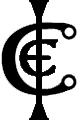
\includegraphics[height=1in]{pictures/Cordo_Siegel.png}
\end{flushright}

\newpage

\section{Animagie}

%\yinipar{D}
Die Animagie ist eine Form oder Schule der Magie, wie Hermetik oder Elementarismus, sie begr"undet sich auf die Interaktion mit Geistern. 
Animagie ist sehr eng mit dem Schamanimus verkn"upft und in der Regel wirken Schamanen und Schamaninnen Spruchzauberei mit Hilfe von Animagie, 
Allerdings sollten diese beiden Schulen nicht miteinander verwechselt werden, sind sie doch zwei f"ur sich gesehen selbstst"andige 
Zweige ohne notwendigen Bezug zueinander.

Die Kraftquelle der Animagie sind Geister, sowohl Elementar- und Naturgeister, als auch Ahnengeister Verstorbener und die Idealisierten 
Vorstellungen von Tieren also Tiergeister. In der animagischen Spruchmagie werden diese durch standardisierte Gesten, Formeln 
und Komponenten dazu gebracht einen bestimmten Effekt in der diesseitigen Welt zu verursachen, der unseren hermetischen Spr"uchen 
bis aufs Haar gleichen kann, aber nicht mu"s. Zum Beispiel ruft ein Animagier einen Windgeist herbei um den Wind zu entfachen und auf 
seinen Gegner zu werfen, die Wirkung ist identisch mit unserem Windsto"s. Was aber viel verbl"uffender ist, ist das sich der Zaubervorgang 
an sich ebenfalls sehr "ahnelt. Besagter Schamane bei dem ich diesen Zauber beobachten konnte hei"st Chop A und kommt aus Silvanaja, er 
wirkt diesen Zauber in dem er mit einem Fetisch, an dem sich unter anderem auch viele Federn befinden, in Richtung des Gegners wedelt und 
folgende Worte rezitiert: „Rad susak vad jak“ (rein phonetische Wiedergabe) die laut 
seiner Au"sage soviel hei"sen wie „komm Wind auf Feind“. Um nicht zu sehr in die Magietheorie abzugleiten werde ich an dieser Stelle nicht 
weiter auf Gemeinsamkeiten eingehen sondern "uberlasse dieses Thema einer zuk"unftigen Vorlesung. Wie der geneigte Leser aber dennoch entnehmen 
kann k"onnen viele bekannte Spruchzauber aus der Hermetik ebenfalls in gleicher Wirkungsweise von der Animagie nachgeahmt werden. Ich pers"onlich 
wurde bereits Zeuge von erfolgreichen Anwendungen "aquivalenter Zauber zu „mentaler Dolch“, „Magiespiegel“, „Furcht“ und einem Feuerball wobei 
erstere zwei wohl zu den kompliziertesten Spr"uchen z"ahlen die die hermetische Spruchzauberei zu bieten hat und somit die Vermutung nahe liegt 
das solch eine Nachahmung mit allen Spr"uchen m"oglich ist.

Die Ritualmagie der Animagier ist weitaus komplizierter, wie es in jeder Magierichtung der Fall ist und da ich bis jetzt noch nicht die Ehre 
hatte einem reinen Animagus bei einem Ritual beizuwohnen halten sich meine Kenntnisse dar"uber auch sehr in Grenzen. An diesem Punkt sei 
lediglich angemerkt das Animagie sich sehr oft mit anderen Traditionen "uberschneidet, teilweise sogar mit Fachbereichen der Hermetik. 
Elementargeister, sind z.B. die Schnittstelle zwischen Animagie und Elementarismus, Naturgeister, die zum Druiden und Hexentum und zur 
allgemeinen Naturmagie. Ahnengeister schlie"slich schlie"sen die Br"ucke zur Nekromantie, einem Weg unserer Hermetik. 
Das hei"st, dass jede Tradition wohl ihren Weg hat in gewi"ser Weise durch Rituale Animagie zu wirken und mit Geistern in Verbindung zu treten.\\

Florian Phelleas Ph"onixflug, Bund zu Ayd`Owl im Jahre 254 nach Jeldrik

\newpage

\section{Oktagon}

\centerline{\huge{Eine magiefreie Zone im Oktagon}}
\begin{flushright}
von Cordobayan
\end{flushright} \setlength{\columnseprule}{0.5pt}
\begin{multicols}{2}
Allerlei Vorhaben bedarf mitunter der Anwendung einer geradezu filigranen Dosis an
arkaner Macht. Vor allem bei der Bearbeitung, Manipulation oder Erschaffung von
Gegenständen ist jede Störung der genau bemessenen Menge von Magie, an strikt
vorgegebenen Stellen des Objektes, unbedingt zu vermeiden.

\includegraphics[height=4cm]{pictures/Gitter_roh.png}

Nun lehrt uns die Thaumgitter-Theorie, dass jedwede Existensebene mit den Strängen der
Magie durchzogen ist, welche sich in Knotenpunkten überschneiden. Auf diesen Bahnen
fließt ständig freie Magie, die von Magieanwendern zur Wirkung herangezogen und gelenkt
wird. Es ist also immer damit zu rechnen, dass ungelenkte Ströme an eben jenem Ort vorbei
fließen, an dem man seine Magie zu wirken versucht.

Um die Wahrscheinlichkeit eines Fehlschlages bei besonders diffizilen Anwendungen nun
signifikant zu senken, ist es angeraten, einen Bereich zu schaffen, an welchem nur solche
Magie existiert, die willentlich dort eingebracht wird.

Um dies zu bewerkstelligen, macht man sich die Kraft des Oktagramms zu nutze. Dieses ist
in der Lage, eine Masche des Thaumgitters derart aufzuspannen, dass die Ströme der Macht
ohne auf Widerstand zu treffen um das ihm innewohnende Oktagon herum geleitet werden. Die
Ausführung gestaltet sich wie folgt.

Zur Orientierung konstruiere der Anwender mit profanen Mitteln ein Hilfsoktagramm, dessen
inneres Oktagon die gewünschte Größe hat, und in dessen Zentrum sich eine natürliche
Masche des Gitternetzes befindet. Nun muss diese Masche aufgespreizt werden. Dazu
visualisiere man sich das Gitter und bringe nacheinander die Oktronae in das Innere der
Masche, und spanne das Gitter soweit auf, bis ein Kreuzungspunkt des Hilfsoktagramms
erreicht ist.

\includegraphics[height=4cm]{pictures/Gitter_okt.png}
Dabei wird an jenem Punkt begonnen, welcher vom Anwender am weitesten entfernt ist, und
mit dem jeweils rechtsherum dritten fortgefahren, bis auch das achte Oktron etabliert und
das Oktagon vollständig ist.\\
Ein Oktron ist hierbei ein kleiner Gegenstand, welcher von einer Affinität zu magischen
Strömen geprägt ist und die Manifestation eines Gitterknotens aufnehmen soll.

Um nun Inneren Magie zu wirken, muss an den Oktronae angesetzt und willentlich eine
Verbindung ins Oktagon hinein etabliert werden, über welche man seine Macht dann leiten
kann.

Zu beachten ist weiterhin, dass der Wille jedes Magieanwenders diese \textit{Umleitung} zu
durchbrechen vermag, da dies explizit vorgesehen ist. Es ist auf diese Art demnach keine
wirkungsvolle Barriere gegen Magieeinwirkung möglich, sondern lediglich eine Abschirmung
gegen ungelenkte Magieströme.\\
\\
Außerdem ist die Stabilität der Konstruktion nur bei verhältnismäßig kleinem Umfang
verlässlich, da bei größeren Arealen enorme Belastungen auftreten können und gewöhnlich
auch werden. Zur Veranschaulichung sei darauf hingewiesen, dass ein sehr großes Oktagon
im Allgemeinen nicht nur eine, sondern eine wesentlich größere Anzahl von Maschen
ausdehnen würde. Gewöhnlich wird eine Masche innerhalb der acht sie umgebenden Maschen
aufgespannt. Schon in der nächsten Stufe der Ausdehnung würden die inneren neun Maschen
in darum liegenden sechzehn hineingeschoben. Somit ist dann aber eine wesentlich größere
Menge an magischem Fluss zu erwarten, der umgelenkt werden müsste.

Die angestrebte Größe des abzuschirmenden Gebietes sollte demnach an der vor Ort
aufgefundenen Größe der Maschen des Thaumgitters orientiert werden.

Cordobayan
\end{multicols}

\begin{flushright}
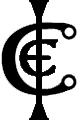
\includegraphics[height=1in]{pictures/Cordo_Siegel.png}
\end{flushright}

\newpage


\chapter{Condra}

\section{S"udlande von Condra}

Bericht "uber die Reise in die S"udlande von Condra.

Sehr geehrter Prytanus Andariel Dagonett,

vor einigen Tagen beteiligte ich mich an einer Expedition der Sturmfalken in die Gebiete s"udlich von Axnom. Dabei ist ein Daimonisches Wesen aus einem Jahrhunderte alten 
Gef"angnis befreit worden und streift seit dem durch die Retekberge. Da Walpurga von Auenbruch offensichtlich zu einer der ehemaligen Wirte des Ythid Darathai geh"orte wollte 
ich euch zus"atzliche Informationen, additiv zu denen, die ihr sicher von den Sturmfalken erhalten werdet, zukommen lassen. Au"serdem stehe ich euch nat"urlich gerne f"ur 
jedwede Fragen bez"uglich der magischen Analysis dieses Vorgangs zur Verf"ugung, sollten die der Armee nicht ausreichen.

Mit freundlichen Gr"u"sen
Florian Phelleas Ph"onixflug, Adeptus des Bundes zu Ayd Owl

\newpage

\textbf{Bericht "uber die Reise in die S"udlande von Condra.}\\

%\yinipar{E}
Erste Woche des siebenten Mondes des Jahres 256 nach Jeldrik. Ihre Markgr"afliche Hoheit Jerevan von Arkenwald schlo"s sich mit seiner Frau Gemahlin und seinem Gefolge 
einer Expedition der Condrianischen Armee in die Lande s"udlich von Axnom in Condra an. Soweit ich mich erinnern kann war der Sinn der Expedition einen alten Posten der Armee, 
Sternwacht gehei"sen, wieder zu finden und neu zu bemannen, doch er sollte im Laufe der Dinge nicht weiter intere"sant werden.
Froh wieder in Condra zu sein und bald meine Freunde wiederzusehen geno"s ich die Reise, bis wir auf die erste Leiche am Wegesrand stie"sen. Es war ein Mann in fremde Kleidung 
geh"ullt, mit einem vermummten Gesicht, wie ich es bis jetzt nur in Samarkant gesehen habe. Er wurde mit einer Handvoll Heimaterde und einer Schriftrolle, die ein Gedicht enthielt, in einen Baum gelegt. Offensichtlich der Totenritus dieser Leute. Die Expedition reiste weiter und erreichte eine kleine H"utte, die an einem Felshang erbaut worden und offensichtlich das einzige "uberbleibsel der gesuchten Grenzwacht war. In dieser H"utte lebten zwei kleine M"adchen ganz f"ur sich alleine, die lediglich von einem eher tumben Dorftrottel besucht wurden, der ihnen Windspiele „gegen die b"osen Geister“ schenkte.
Wie wir nach einiger Resch"arsche herausfanden waren diese M"adchen die T"ochter eines m"achtigen Magiers und einer Hexe, die vor Jahrhunderten hier lebten. Der Magier widmete sein Lebenswerk dem Versuch den D"amonen Ythid Darathai zu bannen, was ihm schlie"slich auch gelang. Doch bei dem Bann verlor er sein Leben und kehrte nur noch als Geist jeden Abend zur"uck, um sich um seine beiden unsterblichen, alterslosen T"ochter zu k"ummern.
Der Mann hatte den D"amonen mit f"unf Ketten und einem Ritual in einen Felsen gebannt, da er eine Exvocation f"ur unm"oglich hielt. Als wir dort eintrafen fanden wir nur noch eine dieser Ketten aus einer Adamantium/Gold/Stahl Legierung vor, welche sp"ater allerdings ebenfalls abhanden kam. Die Turbantr"ager begehrten wohl ebenfalls diese Ketten und entf"uhrten zwei unserer Mitreisenden. Ein unvorsichtiger Krieger "ubergab ihnen dann unserer Kette im Austausch gegen das Leben der Geiseln. Eine andere Kette hatten sie wohl schon fr"uher in ihre H"ande gebracht, indem sie sie ein paar streunenden Goblins abgenommen hatten.
Diese Leute drangen unter Waffengewalt in das provisorisch errichtete Lager am Fu"se des Felsens ein und warfen einen Blick in den magischen Kerker des Ythid Darathai, wohl um sich zu "uberzeugen, da"s sie den Daimonen dort tats"achlich vorfanden und das die Ketten ihre Wirkung taten. Sie zogen nach der Sichtung des Daimonen voller Panik gepackt wieder von dannen, ohne, da"s wir sie angriffen.
Orks hatten sich den starken Nodice Astralis des Gef"angni"ses schon vor Wochen zu Nutze gemacht um ihm Kraft zu entziehen. Diese Kraft lenkten sie um und nutzten sie um Fr"uchte wachsen zu lassen, in denen diese Magische Macht konzentriert war. Aus den Kernen dieser Fr"uchte lie"s sich ein hochpotentes Gift, gegen Astrale Wesen gewinnen, was wir auch taten um dem Daimonen entgegenzutreten.
Durch das Tagebuch des Magiers und den Ausk"unften der kleinen M"adchen erkannten wir nun das wahre Ausma"s des Problems und machten uns bereit ihm entgegenzutreten. Unter gro"sen Opfern gelang es uns die zwei verbleibenden Ketten in unseren Besitz zu bringen. Doch es erschienen zwei Geister, die sich uns als Schutzgeister der M"adchen vorstellte und unser Vertrauen gewannen. Doch in Wahrheit waren sie vom D"amonen geschickt worden um die Orks, oder besser gesagt deren Schamanen unter ihre Kontrolle zu bringen. Wir f"uhrten die Beiden Geister, weil wir es nicht besser wu"sten, zu den Orks und sie beherrschten deren Schamanen. Dann zogen die Orks gegen uns in den Kampf und befreiten Ythid Darathai aus seinem Gef"angnis. Wir mu"sten hilflos mitansehen, wie eines der beiden M"adchen get"otet und das andere Verst"ummelt wurde. Auch mehrere Mitstreiter von uns lie"sen ihr Leben auf diesem Schlachtfeld.
Geschlagen floh die Expedition aus den Landen S"udlich von Axnom zur"uck nach Condra und wir mu"sten zusehen wie der Daimon seine Freiheit wiedererrang.

\newpage


Anbei eine Abschrift des Tagebuches, des besagten Magiers:

\vspace{5mm}

Dies ist ein Traktat "uber den Einen, der „Verr"ater, „Bruderm"order“ und Ythid Darathai gehei"sen wird, eine d"amonische Wesenheit gro"ser Macht.
Der Bruderm"order erscheint nur selten in gestaltlicher Form eines von Knochen ummantelten Wesens mit einem entarteten Kopf, der einer widernat"urlichen Kreuzung aus Mensch und Insekt gleicht. Wenn er dies tut, so ist er jedoch von gro"ser Kraft und beinahe unbesiegbar, da es aus jeder gegen ihn aufgebrachten negativen Emotion oder Handlung neue Kraft beziehen kann.
Sein Vorgehen ist stets "ahnlich: Immer versucht er, die Kontrolle "uber eine Minorit"at aufzubauen, die er dann gegeneinander und gegen Freunde, Verwandte und Wohlt"ater zu hetzen. Aus dieser Ballung von Verrat, Mi"strauen und Ha"s zieht er seine Kraft.
Der Daimon erschien zum ersten Mal in dokumentierter Form auf einem Inselreich im Norden, einem Land namens Neka und dort in einem kleinen Dorf an der Grenze zweier „Provinzen“. Der Daimon trat in Form einer Stimme in Erscheinung „die einen jungen Mann mit falschen Versprechungen und daimonenhaften Kr"aften“ unter ihre Kontrolle brachte. Morde und Diebst"ahle waren an der Tagesordnung und bald schon konnte er seine Kr"afte auf die ganze Dorfgemeinschaft ausbreiten. Nachdem alle, die sich seinem Wirken in den Weg gestellt hatten aus demselben ger"aumt waren, begannen die Raubz"uge in der Umgebung. Hier wurden die Priester des dortigen Feuergottes und einige Magier der gr"o"sten Akademie auf das Ph"anomen aufmerksam, die das ganze Dorf mit Feuer und Schwert ausmerzten, nicht jedoch ohne eine Alnalyse der Kreatur vorzunehmen und ihre Pr"asenz in ganzen Land auszuradieren.
Ich spreche von „dokumentiert“ doch haben wir erfahren, da"s auch den Elfen und Zwergen ein Daimon mit "au"serst "ahnlicher Machart bekannt ist.
Die n"achste Sichtung fand in Jashra statt, einer Stadt in Betheuer. Dort beeinflu"ste er den dortigen Grafen dazu, sich zu einem Despoten aufzuschwingen, der nur durch einen Aufstand der B"urgerlichen gest"urzt wurde. Offenbahr war sich der Verr"ater nicht sicher, wie weit er gehen k"onnte. Ger"uchteweise wurde die Kreatur sowohl identifiziert, wie auch ausgeschaltet, durch einige Elfen, die sich dem Aufstand angeschlo"sen hatten.
All dies habe ich von meinem Meister erfahren, der einen Gro"steil seines Lebens in diesem Neka verbracht hat und als Schiffbr"uchiger die Gestaden Condra erreichte. Auch er hatte nie von diesem Land hier geh"ort. Bald war er als f"ahiger Kenner der magischen Kunst bekannt.
Nach ihrem R"uckschlag in Betheuer mu"ste sich der Bruderm"order anscheinend einige Jahre erholen und sich am Ha"s der Welt m"asten um wieder zu Kr"aften zu kommen. Sieben Jahre sp"ater, ich war inzwischen Lehrling meines Meisters geworden , startete der Daimon seinen bisher letzten Versuch der Korruption.
Die Akademie Condras, das Lied der Harmonie, war erst wenige Jahre zuvor aus einer Kooperative von Hexen und Druiden hervorgegenagen. Die Hexe Walpurga von Auenbruch war eine verlockende Beute. Soweit wir herausfanden war dies das erste Mal, da"s die Kreatur direkt von einer Person besitzt nahm. Entweder werden seine Kr"afte immer st"arker, oder er pa"st sein Vorgehen immer mehr der menschlichen Kultur an. "uber die Leiterin konnte er die Aktionen der jungen Akademie lenken und war durch die Magi besser gesch"utzt als in Betheuer. Mein Meister, der wohl schon l"anger auf der Jagt nach dem Bruderm"order ist, erkannte jedoch dessen Wirken. Gemeinsam mit einigen abtr"unnigen Mitgliedern der Akademie gelang es uns, den Daimon in die Enge zu treiben. Es kam zum Kampf in den Mauern der Akademie als unsere kleine Gruppe bis in die Gem"acher von Auenbruch vordringen konnte, wo wir den Verr"ater stellten.
Die Magier sollten ihn besch"aftigen, w"ahrend mein Meister die Bese"sene von der verderbten Pr"asenz reinigen wollte. Meine Aufgabe war es, die Muster des Daimons zu erforschen, um so zu dem wichtigsten Schl"u"sel im Kampf gegen ihn zu kommen: Sein wahrer Name.
Doch irgendwie gelang es dem D"aimonen, sich aus dem K"orper der Hexe heraus zu manifestieren und uns anzugreifen. Mein Meister war das erste Opfer, doch mit letzter Kraft konnte er ein Portal in eine andere Sph"are "offnen, welches den K"orper des Verr"aters verschlang. Ich selbst kam mit einem verkr"uppelten Bein davon, doch drei unserer Helfer wurden ebenfalls fortgeri"sen. Das schlimmste Bild bot sich jedoch mir, da ich mich der Magia Clarobservantia astralis bediente: Auch wenn der K"orper der Kreatur vernichtet wurde, so weilt ihr verdorbener, wenn auch geschw"achter Geistk"orper immer noch in dieser Welt und wird sich bald neue Macht verschaffen wollen. Dieses Monster mu"s unter allen Umst"anden davon abgehalten werden diese Welt wieder zu verpesten, denn ich f"urchte, diesmal werden wir ihn nicht mehr so leicht aufhalten k"onnen. Aber bereite dich auf einen harten Kampf vor, Bruderm"order, denn ich kenne dich jetzt: (hier fanden wir seinen Namen)

\vspace{10mm}

So kam es, da"s der Bruderm"order einen Leib schuf, in dem gebunden sein faulender Geist weilen sollte.
So m"achtig dieser Leib auch sein mochte, so offenbahrte er doch auch zgleich die Schw"ache des Verdorbenen.
In Fleich gebunden war er verwundbar und konnte durch simple Formen der Magia Combativa attakiert werden.
Diese Wunden schlo"sen sich jedoch viele Male, immer schneller verheilte sein brennendes Fleisch. Aus diesem Wissen erwachte ein Plan in mir, um diesen schlimmsten unserer Feinde endg"ultig zu "uberwinden. Um dieses Ziel zu erreichen müssen drei Dinge geschehen:
Ad Prima: Ythil-Darathai müsste wieder in seinen fauligen Laib gezwungen werden.
Ad Secundo: M"u"ste sein verr"aterischer Geist von den Amni Astralis getrennt werden.
Ad Tertio: Sowohl sein Geist als auch sein Leib müssen am Ort gehalten werden.

\vspace{10mm}

Alle mir bekannten Schurken der Magia Invocatia bedienen sich hierbei einer gro"sen Anzahl von Munstern, welche Portale und Br"ucken zwischen den Ph"ahren zu schlagen verm"ogen. Abgesehen von der gro"sen Gefahr, die diese fragw"urdige Methode in sich tr"agt und dem gro"sen Schaden, die dem Sph"ahrengef"uge durch diese Praxis zugef"ugt wird, w"are sie in diesem Fall auch nicht sonderlich erfolgreich. Der Verr"ater weilt schon seit langem in dieser Welt, so da"s eine Invocatio aus einer anderen Sph"are zum Scheitern verurteilt w"are.
Ihn zu rufen, wie es einige der fraglichen Hexen- und Druidenzirkel empfehlen birgt ebenfalls Gefahren, da wohl schon das Au"sprechen seines Namens seine Aufmerksamkeit erregt, wie es dem Bruderm"order auch einen Pfad in den Geist des armen Teufels "offnen mag, der unbedacht seinen Namen nennt.
So wir also den Verr"ater nicht auf dem uns bekannten Wege der Invocation rufen k"onnen, so plane ich, mich einer, wenn auch sicheren , so doch wesentlich aufw"andigeren Prozedur zu bedienen:
Der Convocatio Maioris!
Wenn ich den Einen nicht dazu zwingen kann zu erscheinen, so müssen eben alle Alle gerufen werden, falls man dieser Kreatur habhaft werden will.
Bei diesem Ritus wird die Bereitung des Platzes die wohl gr"o"ste Aufmerksamkeit erfordern. So mu"s der Magier zun"achst einen Ort finden, der abseits genug von allen astralen Steigwellen liegt, jedoch einen direkten zugriff zum Intervallum Nodicum erm"oglicht. Die coherrenten Amni der topographischen Substanzschwelle müssen exakt nach 3 entsprechen, wogegen keines der Str"ohmungswerte "uber dem Maximal Werten der Lucianischen Portoaethesica liegen darf. (Care!)
Nach der gr"undlichen Reinigung des Platzes kann mit der Arretierungder Amni begonnen werden.
Die systolischen Spannungswellen müssen jedoch jederzeit die Option haben auf ihrer Maximalamplitude zu schwingen, um eine Anpa"sung von nicht mehr als 375 Omikronparametern pro Mondlauf "au"serst unwarscheinlich zu machen.
Wichtig sei hier zu erw"ahnen, da"s man einene der diametralen Amni zwar verst"arkt, jedoch nicht akkumuliert, da dieser zur sp"ateren Apesation des Ableitung"strohmes genutzt werden mu"s. Nach erfolgreichen Fixierung und Akkumulation kann mit dem Retiskonstrukt begonnen werden, welches dem Gef"uge angeglichen und mit dem Amnis und dessen diastolischen Ladunswert syncronisiert werden mu"s.
Sobald die Syncronisierung begonnen wurde, müssen wir uns dem zentralen Konstrukt zuwenden, reicht es schlie"slich nicht, die Kreatur nur zu rufen. Um jedoch die Matrizen der Fixation in die mannigfaltigen differenten Mani zu integrieren, mu"s zun"achst ein zentraler, am besten leicht erh"ohter Fokuspunkt gefunden werden, an dem die Amni non cogerient werden.
Hier kommt nun das Detis oder Netzkonstrukt ins Spiel, welches mit Hilfe der metaphysischen nominalen E"senzkomponenten, dem „wahren Namen“, des gesuchten Astralleibs der Ma"se der Convocierten heraus zu binden vermag. Als hilfreich zeigt sich ein Fokus, der auch in unserer Sph"are bindende Kr"afte h"atte. Ich habe mich f"ur ein paar Ketten entschieden, welche die vier Gliedma"sen und den Hals der Kreatur binden werden.
Es wurde eine 15:4:1 Legierung aus Stahl, Gold und Adamatium verwendet, welche ich mir von den Zwergen in Axnom fertigen lie"s.
Nach der Artefaktbindung von Augustus Runethal mu"s die E"senzkomponente (Der „Name“) in die bindenden Foki gepr"agt werden, da ein astraler Leib in jedem Fall von seiner eigenen Struktur gehalten werden kann.. Auch sollte in diesem Arbeit"schritt die Kommunikationsverbindung zum immigrierenden Amnus geschlagen werden, verbunden mit einer Matrix, die dessen Aktivit"at einstellt, sobald die Ketten eine posititve Resonanz abgeben. (Verdammt jetzt mu"s ich auch noch die Tinte wechseln!)
Danach mu"s der Magier eine manuelle Abschaltung vornehmen, welche den emmigrierenden Amnus betrifft, da sonst m"oglicherweise noch andere Dinge in der N"ahe des Fokus an das Gef"uge der Gegend gebunden werden k"onnten.
Durch die Trennung wird jeder innerhalb des Kreises vom astralen Raum abgeschnitten und der D"amon gefangen. Au"serdem werden durch das Zusammenspiel der Ketten und des Astralkonstruktes (s.u.) die Heilungskr"afte der Kreatur eingeschr"ankt. Ich bin zwar nich sicher, ob man genug arkane Macht oder Waffengewalt aufbringen kann um ihn zu zerst"oren, aber gottseidank wird das nicht n"otig sein, sobald das Konstrukt seine Arbeit tut.
Die Ketten sollten sowohl astral als auch physisch in einer Weise angebracht werden, da"s sie in der Lage sind da Wesen zu halten, wobei sich der Astrale Aspekt mit dem Gewebe von selbst verbinden sollte.
So der Bruderm"order also im Fokus Amnium, welches in Form eines Schutzkreises von ausreichender Gr"o"se vorliegt sollte gefangen ist, kann mit dem zweiten Teil der Vernichtung begonnen werden.
Es scheint hilfreich einen Kreis zu w"ahlen, der tats"achlich k"orperliche, wenn m"oglich nat"urliche Komponenten enth"alt, da dies die Bindung noch weiter verst"arkt.
Doch wollen wir nun zur schwierigsten Komponente kommen:
Ich habe seit langem einen weg gesucht, den Geist des Verr"aters zu zerst"oren ohne seinen K"orper zu zerst"oren und den Geist damit wieder freizulassen. Jetzt endlich habe ich eine M"oglichkeit gefunden. Man mu"s ihm die Gelegenheit geben sich selbst zu vernichten!
Eine implodierende, durch temporale und astrale Reizung ausgel"oste Astraltasche, welche gleichzeitig als Leiter fungiert! Jede Kraft, die die Kreatur im Inneren anwendet f"uhrt dazu, da"s sich das Gef"uge doppelt proportinal zur eingesetzten Kraft schlie"st und zusammenzieht, und gleichzeitig jegliche Energie aus dem inneren harmlos ableitet. Je mehr sich die Bestie als wehrt, desto eher wird sie sich selber ausl"oschen!
Um aber sicherzugehen, da"s Ythid Darathai auch wirklich vernichtet wird, wird das Konstrukt auch von alleine enger, was den letzten und schwierigsten Teil der Herstellung darstellt.
Sind alle vorbereiteten Ma"snahmen vollendet, so mu"s der Fokus Amnium an der Stelle der Fe"selung plaziert werden. Der Magus steht in einem kleineren Kreis, welcher mit dem Pentagramma gezeichnet ist und sich zwei und einen halben Schritt vor dem Siegel befindet.
Die Initiation des Ritus ist nun recht einfach, mu"s doch nur der convocative Kraftflu"s gerufen werden und zwar mit folgenden Worten:
Alii aliam in partem feruntur!
Der zweite Annus wird aktiviert mit den Worten:
Spititi timebant, ne circuirentur!
Alles was die Str"ome nun noch hemmt, ist der Fokus selbst und mit folgenden Worten kann endlich das Ende des Bruderm"orders eingel"autet werden:
Portus Annis arcaniterem odenbar 

\newpage

\section{Miasaris Toreville}

%\yinipar{M}
Miasaris Toreville war eine Adepta der Akademie von Nektor. Sie hatte ebenfalls den Kampf gegen die Schatten Grenzbruecks zu ihrem eigenen gemacht und ist im Sp"atsommer 257 nach Jeldrik bei der Errichtung des Walles gestorben.
Statt eine Laudatio zu halten m"ochte ich hier, an dieser Stelle Ihre akademischen Werke ver"offentlichen, da sie zu Lebzeiten nie die Gelegenheit dazu hatte es selber zu tun. Es ist eine Abhandlung "uber die V"olker Condras und eine "uber die Sprache der Orks in Grenzbrueck. Letztere hatte sie in Grenzbrueck stets mit einer Leidenschaft verfolgt, wie ich es selbst bei Sprachwissenschaftlern selten gesehen habe. Ich hoffe sie ruht in Frieden und das wir sie durch ihre Schriften auf ewig im Ged"achni"s behalten werden.

\subsection{V"olker und Wesen Condras}

"uber die V"olker und Wesen Condras

Condra ist, vergleicht man es mit den K"onigreichen der Mittellande, Engonien oder Neka, ein kleines Land, in wenigen Tage durchquert man es zu Pferde, vom sumpfigen Norden zu den Retekbergen, von den Elfenw"aldern im Westen zur Steilk"uste im Osten. Nichtdestotrotz leben auch hier eine Vielzahl der verschiedensten Wesen, die ich, Miyasaris Thoreville aus Nektor, kurz vorstellen will. 

\newpage

\subsubsection{Die Menschen}

%\yinipar{D}
Das zahlenm"a"sig gr"o"ste der kulturschaffenden V"olker Condras (die meisten Gelehrten gehen der Frage, inwiefern man Orks zu diesen z"ahlen kann, wohl absichtlich aus dem Weg – mehr dazu sp"ater). Nach vorsichtigen Sch"atzungen sind weit "uber 90 pro centum der Lebewesen Condras menschlich, das entspricht in absoluten Zahlen etwa 40.000 K"opfen – mangels eines allgemeinen Zensus seit der Nekanerzeit. Da sich zur Siedlungsgeschichte in der fr"uhen vornekanischen Zeit keine Quellen mehr finden lassen, die uns verr"aten, ob es eine urt"umliche Bev"olkerung dieser rauhen Lande gab, bin ich hier auf eine Extrapolation meiner Forschungen zur Sprachenverbreitung angewiesen. Zuallervorderst sei auf das Faktum hingewiesen, da"s Condra und Betheuer wie auch andere L"ander der weiter entfernten Mittellande sich eine Sprache teilen. Meine Vermutung ist, da"s diese Sprache mit den dranaischen Fl"uchtlingen aus Neka hierher kam. In Betheuer gibt es sogar schriftliche Quellen, die die These, 'Condrianisch' w"
are die Sprache der Nekaner gewesen, unterst"utzen. M"ogen die patriotischen Zweifler auch jede Behauptung, wir w"aren mit den Feueranbetern verwandt, weit von sich weisen, so bleibe ich doch dabei. Denn auch das Gegenargument, Neka h"atte doch fr"uher “Altnekanisch” gesprochen (uns als Sprache der steinernen Inschriften und pomp"osen Schriftst"ucke bekannt) und w"are erst durch Reisende aus den Mittellanden zu einer anderen Sprache gekommen, halte ich f"ur Unfug. Ein auf die eigene Kultur bis zum Fanatismus stolzes Land wie Neka, das niemals Einwanderung kannte, soll von Fremden etwas "ubernommen haben? Lachhaft! Aber ich schweife ab.
Lokale Dialekte haben sich in dieser kurzen Zeit nicht herausgebildet, vereinzelt h"ort man noch Ankl"ange an die singende Sprechweise der Alineser und unter der Landbev"olkerung vor allem der abgelegenen Wei"squelld"orfer hat eine gewi"se Verschleifung stattgefunden, die in der Gegend um Widdau am st"arksten zu sp"uren ist. Auch regionale Unterschiede im Gem"ut und Alltagskulture sind (noch) nicht festzustellen. Der s"udliche Condrianer ist, wohl durch die in der Vergangenheit h"aufigen Orkangriffe und ein Leben in st"andiger Verteidigungsbereitschaft, wortkarger und verschlo"sener, der n"ordliche Condrianer der Wei"sspitzen und Venne ist eigenbr"otlerisch aber herzlich.
Die Statur ist gleich, m"annliche Condrianer werden im Durchschnitt 175 Zentimeter gro"s, Frauen 165 Zentimeter (Stadtbewohner gr"o"ser). Im Durchschnitt werden Stadtbewohner 70 Jahre alt, doch 80 pro centum aller Menschen leben als Bauern und Handwerker auf dem Land, der Rest verteilt sich auf die St"adte Tharemis, Schieferbruch und Nektor. Das Hauptnahrungsmittel ist Getreide (Hafer, Weizen, Gerste) vor allem aber auch Erdknollen aller Art, die der Witterung entsprechend besser wachsen und im Winter eingekellert werden k"onnen. Da Condra keine nennenswerten Bodensch"atze sein Eigen nennt (einige kleinere Vorkommen in den Wei"sspitzen, die Minen der Retekberge sind fest in Zwergenhand), mu"s Metall importiert werden – was sich auch in der Au"stattung der “Armee” niederschl"agt, die nur dicke Tuchr"ustungen und einige wenige Kettenhemden aufbieten kann. Plattenpanzer sind teure Importware aus Betheuer oder den Mittelanden. Der technische Stand Condras ist der, da"s Buchdruck, Uhrwerke, Kompa"s und andere 
Linsensysteme bereits Verbreitung gefunden haben, es aber  immer noch eine kleine Sensation war, als Sendrian Schneeloh vor einem Jahrzehnt in Tharemis eine Walkm"uhle f"ur Wolltuche er"offnete. Die meisten Condrianer leben ein einfaches Leben, angepa"st an die Jahreszeiten und stark lokal gebunden, doch - nicht zuletzt verst"arkt duch den Hydracorglauben – sind sie freiheitsliebend, aufrecht, wenn auch nicht immer wahrheitsliebend und vor allem von einer schroffen Direktheit, die in H"oflichkeitskulturen wie der Betheuers undenkbar w"are.
Der nekanische Versuch, Condra ein hierarchisches System aufzudr"ucken, kann auch in dieser Hinsicht als gescheitert angesehen werden. Condrianer folgen nur denen, die etwas f"ur sie tun und die sie respektieren k"onnen. Solchen Respekt kann die Hydracorkirche einfordern, denn der Hydracorglaube ist de facto die Staatsreligion. "uber das F"ur und Wider einen Personalunion von Regierung und geistigen Herrschaft werde ich mich hier nicht auslassen, nur soviel, da"s der Klerus sehr viele F"aden in der Hand h"alt und auch, wie ich erfahren mu"ste, viel Wissen unter Verschlag. 
Hydracor ist Gott des Wassers, Wandels und der Welt in ihrer wilden Form, daher ist es nicht verwunderlich, da"s Condra sein Augenmerk niemals auf die Bezwingung der Natur richtete wie Neka mit seinen Monumentalbauten. F"ur eine genauere Beschreibung dieser Glaubenslehre verweise ich auf die Schriften des nekanischen Forschers und gesch"atzten Kollegen Jakobius Sonnau. 

Nachtrag: Mir ist zu Ohren gekommen, da"s es im tiefen S"uden, noch unterhalb der Orklande, in w"armeren Gefilden, ein Eingeborenenvolk geben soll, das helle Kleidung tr"agt und eine andere Sprache spricht. Aber ob dieser Menschenstamm ebenfalls eingewandert ist oder nicht, kann ich mangels Informationen nicht sagen. 

\newpage

\subsubsection{Orks}

%\yinipar{I}
In Condra waren einmal zwei gro"se Orkst"amme beheimatet: Die Gr"unorks und die Braunorks.  Nachdem die Gr"unorks jedoch aus dem Kernland vertrieben worden waren und von den Braunorks 
aufgerieben wurden, finden sich nur noch wenige Gr"une, die meist in kleinen Gruppen durch die W"alder schweifen oder sich bei Menschen als billige Arbeitskr"afte verdingen. Die Braunorks jedoch sind umso gef"ahrlicher geworden. Zwar haben sie nicht, wie damals in den Orkkriegen, den gesamten S"uden "uberrannt, aber bis vor kurzem waren die S"udrouten und alles Land unter den Retekbergen orkverseucht. Geholfen hat ihnen bei der Verw"ustung des S"udens, da"s ihre Schamanen, die einzigen die Magie verwenden k"onnen, niedere D"amonen unter ihre Kontrolle brachten. Diese D"amonen werden wohl in Blutritualen mit ordin"aren Braunorks verschmolzen, woraus dann die monstr"osen Rotorks entstehen, deren Geist durch das Ritual zerst"ort, zu w"utenden Berserkern werden, die auch unter ihren Orkkumpanen eine Spur der Zerst"orung hinterlassen. Im Zustand der Raserei sind sie nur noch durch erfahrene Schamanen zu beherrschen. Sie sind erkennbar an der roten F"arbung ihrer lederartigen Haut, ihren breiten Schultern, ihrer 
Unf"ahigkeit zu sprechen und ihrer f"urchterlichen Kraft. Im Vergleich mit ordin"aren Orks k"ummern sie sich noch weniger um Kleidung, soda"s sie meist nur den ungegerbten Pelz von erlegten Wildtieren am Leib tragen. Gr"une und braune Orks kommen in allen Gr"o"sen und Konstitutionen, die meisten sind allerdings st"ammiger und st"arker als durchschnittliche Menschen. Sie sterben fr"uher, meist bereits nach 20-30 Jahren. Orks ern"ahren sich gr"o"stenteils von Fleisch, dazu von Milch ihrer Viehherden und von wild wachsenden Pflanzen. Ihre Kleidung besteht aus Leder, Pelz und groben Stoffen, Schmuck aus Knochen, Federn und anderen tierischen (und humanoiden) K"orperteilen. Zivilisiertere Gr"unorks bevorzugen allerdings menschliche Kleidung. Ger"ustet sind sie meist entweder mit kr"uden Ansammlungen von Metall, gefundenen menschengefertigten R"ustungen oder Naturmaterialien. Ausgeglichen wird dies, da"s ihre Haut dicker ist als die der Menschen. Ihre Behausungen bestehen bestenfalls aus Erdh"utten und Lederzelten.
 Sie haben eine eigene Sprache, die aus Knurr-, Plosiv und Kehllauten besteht. Eine formelle Schrift kennen nur die Schamanen und einige H"auptlinge. Ger"uchteweise sind die condrianischen Orks degenerierte Nachfahren eines einstmals kulturschaffenden Volkes, das sogar m"achtige Bauwerke erschaffte und eine Bilderschrift sein Eigen nannte, doch sind die Quellen nicht zuverl"a"sig – eine Gruppe Abenteurer, die mir von einem Zusammentreffen mit einem solchen zivilisierten Ork erz"ahlte, sehe ich nicht als Beweis, vor allem angesichts der Tatsache, da"s es keinerlei Grabungsfunde gibt. 
Ein humanoides Volk, von dem ich nicht wei"s, ob es einfach nur orkische Mi"sgeburten sind, sind kleine gr"unh"autige Wesen, mit langen, zur Seite h"angenden Ohren. Sie kommen nur im S"uden vor, werden "au"serst selten gesichtet, daher bin ich inzwischen der Meinung, da"s sie ebenfalls nicht aus Condra stammen. Es soll hier ja auch Feen und Kobolde geben, aber ich habe in meinem ganzen Leben noch keinen zu Gesicht bekommen. 

\newpage

\subsubsection{Zwerge}

%\yinipar{E}
Eines der alten V"olker, das sich nicht lange nach Beginn der Nekanerherrschaft aus den menschlichen Angelegenheiten zur"uckgezogen und in seinem Bergk"onigreich Axnom abgeschottet hat. Zur selben Zeit wurden auch die letzten Minen in den Wei"sspitzen aufgegeben, die, wie der Hohe Rat durch Untersuchungen herausfand, allerdings auch ersch"opft sind. Wie man erkennen kann, sind die Zwerge ein Volk, das ber"uhmt ist f"ur seine handwerklichen F"ahigkeiten. Vor allem in Metallverarbeitung, Bergbau und Feinmechanik (aber auch in der Braukunst) sind ihre Werke ohnesgleichen. Ihre Verbundenheit mit dem Erdboden "au"sert sich darin, da"s sie Wohnh"ohlen oberirdischen H"ausern vorziehen und da"s auch ihre Nahrung subterrane Pflanzen umfa"st.  Zwergische Kleidung unterstreicht ihre Kunst: Harte Formen, die Farben von Stein und Metall, geometrische Muster und Metallst"ucke als Verzierung. Zwerge erreichen eine maximale K"orpergr"o"se von 165 Zentimeter, sind korpulent und kr"aftig gebaut. Ihr gro"ser Stolz 
sind ihre langen B"arte, die bei m"annlichen Zwergen eine stattliche L"ange erreichen k"onnen. Viele, aber nicht alle weiblichen Zwerge haben einen Kinnbart. Beide Geschlechter tragen kunstfertig geflochtene Z"opfe.  Ihre Sprache ist die der Menschen, ob es  einmal eine andere, alte Sprache gegeben hat, ist unbekannt, doch ihre Schrift ist eine andere. Es ist, wie ich herausgefunden habe, eine phonographische Buchstabenschrift, die eckige Runen verwendet, die leicht in Stein zu mei"seln und in Metall zu gravieren sind. Zu den Runen, die Laute repr"asentieren, kommen noch spezielle Zeichen, denn jeder zwergische Titel hat eine Rune, genauso wie die einzelnen Bingen – Reste einer Bildschrift? Die Gesellschaftsform ist stark hierarchisch, mit der K"onigsfamilie an der Spitze, den Meisterschmieden und Meisterbergbauern als Elite. Dazu gibt es noch die Priester der Schmiedegottheit Fulgor, die einzigen, die imstande sind, etwas zu verwenden, was wir Menschen „ klerikale Magie“ nennen w"urden. Das restliche 
Zwergenvolk ist so magisch wie – ein Stein. 

\newpage

\subsubsection{Elfen}

%\yinipar{N}
Nicht viel ist bekannt "uber dieses alte Volk, da sich bereits vor der Nekanerherrschaft die Elfen vollst"andig aus der Menschenwelt zur"uckzogen. Und auch jetzt, da die n"ordlichen Handelsrouten wieder ge"offnet sind, ist der Kontakt eher sp"arlich. Einige wenige junge Elfen haben die W"alder verlassen und leben unter den Menschen. Was sich "uber die Elfen sagen lässt, ist, da"s sie  hochgewachsene Wesen, von schlanker Gestalt, ohne Gesichts- und K"orperbehaarung und mit leicht l"angeren, spitz zulaufenden Ohren sind. Sie sind Meister in der Herstellung feiner leichter Stoffe und Schmuckst"ucke aus weichen Metallen mit organischen Formen.  Ihre Affinit"at zu Magie scheint um einiges h"oher als die der Menschen zu sein, denn unter ihnen gibt es nur wenige, die sie nicht zu gebrauchen scheinen. Elfen altern sehr langsam und ihre Jahre sind ihnen auch nicht anzusehen. Eine eigene Schrift und eine wohlklingende Sprache haben sie, doch hatte ich bis jetzt keine Gelegenheit, mehr als ein paar Wort zu 
erlernen, da ich noch nie einer Elfe begegnet bin, sondern nur Fuhrleuten, die von ihnen durch den Wald geleitet wurden. "uber ihre Geschichte konnte ich ebenfalls nichts in Erfahrung bringen, doch scheinen sie wie die Zwerge bereits vor den Menschen in diesen Landen gelebt haben, da es auch in Betheuer Reste einer elfischen, ebenso naturverbundenen Zivilisation gibt. 

\newpage

\subsubsection{Nazgash}

%\yinipar{A}
Auch wenn einige meiner gesch"atzten Kollegen abstreiten, da"s diese aufrecht laufenden menschengro"sen Echsen mehr sind als Tiere, mu"s ich sie doch erw"ahnen, da sie meiner Ansicht nach zumindest ein paar Anzeichen einer Kultur haben. Erstens tragen sie Kleidung als Schutz gegen die Sonne, die von Menschen gestohlen zu sein scheint, zweitens verwenden sie rudiment"are Werkzeuge aus Holz und Stein sowie menschengefertigte Waffen und drittens scheinen sie zumindest rudiment"ar die menschliche Sprache zu verstehen. Ihre eigene Sprache ist allerdings f"ur uns Menschen absolut unverst"andlich, sie besteht nur aus Zischlauten. Handwerkliche F"ahigkeiten, die "uber den Bau von Nestern und groben Schuhwerk hinausgehen, scheinen sie nicht zu kennen. Wie andere Reptilien legen sie Eier, allerdings wenige pro Weibchen, die danach im Stammesverband um jeden Preis bewacht werden. 'Angef"uhrt' werden die Verb"ande von den "altesten Weibchen, da die M"annchen eine k"urzere Leben"spanne haben. Ihre Lebensr"aume 
sind die S"umpfe der Fenne im Norden und Westen. Den Gebrauch des Feuers scheinen sie nicht zu kennen, daher ist es zumindest mir ein R"atsel, wie sie in der winterlichen K"alte der S"umpfe "uberleben. Sie sind sehr scheu und bevorzugen den Aufenthalt im Schatten, daher wird man selten einen Nazgash zu Gesicht kriegen. Die Farbe ihrer Schuppen geht von gelbgr"un bis zu braungr"un, ob dies ein Zeichen einer Alterung ist, ist mir unbekannt. Ihre Nahrung besteht aus Pflanzen, aber vor allem Fischen, kleineren Reptilien und Insekten. 

\newpage

\subsubsection{andere seltsame Wesen}

Drow, Trolle, Kender und andere seltsame Wesen

Vorweg der Hinweis, da"s alle vorgenannten Wesen nicht urspr"unglich in Condra vorkommen. 

Wilde Trolle, gro"s wie zwei Menschen, wandern manchmal aus dem S"uden ein, aber die letzte Sichtung war von 120 Jahren, auch wenn Reisende schon mal Trolle als Lasttiere mitbrachten. 

Drow kommen aus dem einen weiten H"ohlensystem in Betheuer, wo die Armee selbst mit Hilfe der Sturmfalken nicht eindringen konnte. Zum Gl"uck f"ur die Menschen bleiben diese dunklen Elfen – schwarze Haut, wei"se Haare - meist unterirdisch, da sie Tageslicht nur unter Drogen und unter Schleiern ertragen. Wenn sie an die Oberfl"ache kommen, sind sie grausame, hinterlistige Wesen, den Menschen feindlich und den Elfen ha"serf"ullt gegen"uber, daher werden sie gejagt, wo immer man sie in Betheuer sieht, doch wehe den Menschen, die von ihnen gefangen und versklavt werden. Ihre Gesellschaft ist matriarchalisch, mit Priesterinnen ihrer Spinnengottheit als Elite. "uber ihre Lebensweise und Kulturf"ahigkeiten ist nicht viel bekannt, sie scheinen zumindest Waffen und dunkel gef"arbte Tuche selbstt"atig herzustellen, ihre Gifte sind schrecklich und ihre Magie ist so stark wie die ihrer lichten Verwandten, der Elfen. Ihre Sprache ist h"arter als Elfisch, aber leider hat noch niemand sie erforschen k"onnen. 

Kender, Hobbits, Kobolde und Feenwesen sind in Condra nur als Durchreisende und fremdartige Besucher zu finden. Kender und Hobbits sind kleine spitzohrige Menschen"ahnliche. W"ahrend die ersten die Gestalt von schlanken, aber kleinw"uchsigen Menschen haben, sind die letzteren eher rundlich, mit lockigen Haaren und pelzigen F"u"sen. Kender haben die unschuldige Neugier und das Staunen von Kindern, Hobbits einen uners"attlichen Appetit. Beide V"olker sind nicht daf"ur bekannt, Magie zu kennen, sind aber daf"ur friedfertige, fr"ohliche Wesen. 
Im Gegensatz dazu kann das, was man Kobolde nennt, laut den Sagen fiese Gesellen sein. Die Magie dieser buntgekleideten gr"unh"autige Spitzohren ist von einer anderen Art als die der Menschen, daher k"onnen sie als Feen im Gegensatz zu menschlichen Magiern einfach zwischen ihrer eigenen Welt und der der Menschen hin- und herwechseln. Andere Feenwesen kommen in allen m"oglichen Formen und Farben vor, daher ist  eine allgemeine Au"sage "uber sie nicht m"oglich, doch im Gegensatz zu den Kobolden verlassen sie ihr Reich nur unter ganz besonderen Umst"anden. Ich zumindest habe in meinem gesamten Leben noch nie eine Fee oder einen Kobold gesehen, daher w"are ich geneigt, sie ins Reich der M"archen zu verbannen, wenn meine Freunde mir nicht als Augenzeugen von Treffen mit solchen erz"ahlt h"atten. 

\vspace{10mm}

Miyasaris Toreville

\newpage

\chapter{Grenzbrueck und die Schatten}

%\yinipar{I}
In Grenzbrueck tobt seit Jahren der Krieg gegen die Schatten. Ich wurde bereits in den Jahren meines Adeptentums an der Akademia zu Ayd'Owl in diesen Konflikt verwickelt und seit dem immer tiefer darin verstrickt. Ich habe viele Bekannte und Freunde an Morbus verlohren und auch mehr als einmal habe ich selbst an der Schwelle des Todes oder noch Schlimmerem gestanden. Hier ver"offentliche ich das Wissen, da"s wir in den Jahren gesammelt haben, um es nachfolgenden Generationen zu erhalten sollte ich einmal nicht mehr in der Lage sein es zu teilen.


\section{Von Miasaris Toreville}

%\yinipar{M}
Miasaris Toreville war eine Adepta der Akademie von Nektor. Sie hatte ebenfalls den Kampf gegen die Schatten Grenzbruecks zu ihrem eigenen gemacht und ist im Sp"atsommer 257 nach Jeldrik bei der Errichtung des Walles gestorben.
Statt eine Laudatio zu halten m"ochte ich hier, an dieser Stelle Ihre akademischen Werke ver"offentlichen, da sie zu Lebzeiten nie die Gelegenheit dazu hatte es selber zu tun. Es ist eine Abhandlung "uber die V"olker Condras und eine "uber die Sprache der Orks in Grenzbrueck. Letztere hatte sie in Grenzbrueck stets mit einer Leidenschaft verfolgt, wie ich es selbst bei Sprachwissenschaftlern selten gesehen habe. Ich hoffe sie ruht in Frieden und das wir sie durch ihre Schriften auf ewig im Ged"achni"s behalten werden.

\newpage

\subsection{Grenzbr"ucker Orkisch}

Grenzbr"ucker Orkisch – Die ersten Worte

%\yinipar{D}
Diese kurze Liste entstand w"ahrend meiner letzten Reise nach Grenzbr"uck. Wieder einmal hatten wir Morbus Pl"ane vereitelt und auch wenn ich beinahe dabei gestorben w"are, als mich der Fluch seiner Dienerin Lechata, der Frau ohne Gesicht traf, war es doch wert, denn zum ersten Mal hatte ich einen – tempor"ar friedfertigen - Ork namens Tullamok gefunden, der bereit war, mir einige Worte beizubringen. Ich bedaure zutiefst, da"s dieser mein Lehrer nach nicht einmal einer Stunde von Kriegern eines feindlichen Braunhautstammes umgebracht wurde und ich ihn nicht retten konnte. Die Orks, die wir davor getroffen hatten, waren entweder die von Morbus pervertierten Lok Ashtar gewesen oder hatten uns angegriffen und waren von den menschlichen Verteidigern sofort niedergemacht worden. 

Sobald sich mir die Gelegenheit erneut bietet werde ich diese Liste hoffentlich zu einem kleinen Wortschatz ausarbeiten k"onnen. Die F"ahigkeit, mit den Orks zu kommunizieren, darf nicht zu gering gesch"atzt werden, hat sie doch schon einmal Leben gerettet. Sei es, um mit den Orks zu verhandeln, sie und Morbus zu entzweien oder sie zu belauschen – die Kenntnis  ihrer Sprache wird ein Schritt auf dem Weg zur Vernichtung des "ubels der Schattenlande sein.

Miyasaris Thoreville, Tharemis im Jahre 5 n.d.B. (entspricht 256 n Jeldrik Anmerkung Ph"onixflug)

Die Sprache der Orks ist, wie man sehen wird, voller harter Laute, vor allem -k und -r. Wenn sie gesprochen wird, sollte auch darauf geachtet werden, diese Laute zu rollen, knurren und herauszusto"sen. 

Grenzbr"ucker Orkisch scheint eine aglutinierende Silbensprache zu sein, jede Silbe ist ein Wort und  tr"agt  eine Bedeutung. Weitere Bedeutungen entstehen durch Zusammensetzungen der Silben/Worte als Komposita und durch Anhang von Silben. Verben werden wohl nicht flektiert, sondern durch Hinzunahme weiterer Worte wie 'fr"uher/gestern' oder 'morgen/zuk"unftig' in verschiedene Tempi gesetzt. Eine festgelegte Wortreihenfolge gibt es nicht, aber meist werden handelnde Personen vor die Verben gesetzt. 

\newpage

Pronomen:\\

ar =  ich \\
ur = du \\

('sie' wird durch eine Benennung der Gruppe oder einzelnen Person gebildet, "uber die geredet wird)\\

-nan - mehrzahl, alle, viele \\
arnan = wir \\
urnan = ihr \\

artok = mein \\
urtok = dein \\
\newpage
Verben:\\

- tok = Verb des Haben und Besitzens.\\

kramm = fre"sen \\
nirkramm = trinken \\

- nir =  ! verneinung/umkehrung dessen, was davor oder dahinter steht\\

hosch = k"ampfen \\
rakk - jagen \\

\newpage

Nomen: \\
ork = Ork\\ 
homm = Mensch\\
kat = Katze \\
nirkat = Ratte/Maus  \\
mago = Hexe \\
pak = Waffe\\
gorr(o) = gro"s \\
schakk = Beh"alter? Ding?\\
Sulk = Feuer \\
gach = Rache \\
nakk = Krieg \\
hok = Feind  \\
nirhok = Freund\\
kar = Geist/Magie\\ 
karoschakk = Magie(ding)\\
Mok Gakhan = Die Maske (Morbus' Artefakt)\\
ham = Holz \\
tul? tuul? = Dorf? H"utte? Blut? Tod? \\

Wie man sieht, k"onnen Worte durch ein zus"atzlich eingef"ugtes 'o' besser sprechbar gemacht werden, sowohl die Form 'karschakk' als auch 'karoschakk' sind richtig. \\
Miyasaris Toreville
\newpage

\section{ Auszuege aus der Thesys}

Vorwort:\\
%\yinipar{D}
Die Thesys ist ein Dokument, da"s uns Wissen ueber vergangene und zukuenftige Geschehni"se in Verbindung mit dem Schatten verspricht, der Grenzbrueck befallen hat. 
Wann immer uns ihre Anwesenheit offenbahr wurde und ein neues Kapitel in ihr zu oeffnen war schrieben wir ihren Inhalt nieder um sie der Nachwelt zu erhalten. 
Wenige Paszagen und Stuecke der Thesys wurden uns offenbahr und dies sind die Abschriften, die von wenigen Mutigen gemacht wurden.\\
Sie repaesentiert unser Wissen im Sommer des Jahres 258 nach Jeldrik und erhebt keinen Anspruch auf Vollstaendigkeyt, da sie aus vielen verschiedenen Quellen 
und unter besonderen und wiedrigen Umstaenden zusammen getragen wurde.
\newpage

\begin{center}
\begin{Huge}Im Gedenken an:\\\end{Huge}

\vspace{10mm}

Aaron - Diener des Ewigen\\
Felian - Held\\
Harkon - Knappe Grenzbruecks\\
Varn Chamounde – Adeptus Cantus Harmonae\\
Andor - Adeptus Cantus Harmonae\\
Grunas - Wolf der Armee Condras\\
Tarik - Soldat der Armee Condras\\
Jonan - Soldat der Armee Condras\\
Kira - Heldin\\
Illayda Wolfslauf - Archontin Condras\\
Fisken - Unnabhaengiger Condras\\
Miyasaris Toreville - Adepta der Academia zu Nektor\\
\end{center}

ebenso wie die zahllosen Soldaten und Kriegern aus Grenzbrueck, Engonien, Condra und vielen anderen Laendern, die ihr Leben im Kampf gegen die Schatten verlohren haben.

Anmerkung der II. Edition:\
In der unrsprünglichen Ausgabe befanden sich an dieser Stelle mehrere ausführliche Auszüge aus der Thesis. Aufgrund Ihres lokalen und temporalen Bezuges möchte ich sie
für die II. Edition ausspahren und durch zusätzliche Artikel von allgemeiner Relevanz ersetzen.


\newpage



\chapter{sonstige Publikationen}

\section{Grundlagen der Alchemie}


Grundlagen der Alchemie


Von Thalian Sanderfels

\subsection{Einführung}

Mit diesem Werke soll eine kurze Einführung in die Grundlagen der Alchimie und damit ein erster Überblick über die Thematik gegeben werden.\
Die Alchimie basiert auf dem Systeme der vier Elemente: Feuer, Wasser, Erde und Luft. Diese vier Elemente sind der Ursprung und die Grundsubstanz unserer Welt, alles bestehet 
aus den vier Elementen und setzt sich aus jenen zusammen. Sie sind die Grundlage allen Seins. \
Sie sind die Grundsubstanz der Existenz und bilden  ihre Bausteine. Die Elemente existieren in ihrer reinen Form jedoch nicht in unserer Welt, sondern immer nur als Verbindung 
miteinander. So gibt es kein reines Feuer sondern nur warme Luft, warmes Wasser oder warme Erde. Die Extreme, die Reinform eines einzigen Elements findet man nicht in unserer 
Welt. Die Dinge definieren sich also über die Elemete aus denen sie bestehen. Das einzige was die Dinge der Welt voneinander unterscheidet ist das Verhältnis der Elemente in 
ihnen. Alles lasset sich auf die vier Elemente reduzieren, sie sind die letzten und kleinsten Teile aus den sich alles zusammensetzt. 
So isset es theoretisch denn auch möglich durch die Alchimie alle Dinge herzustellen und einen jeden Stoff in einen anderen zu überführen, das difficile an jener Aufgabe ist 
es jedoch, dass genau Verhältnis zu finden, da nur durch eine perfekte Änderung das gewünschte Ergebnis erreicht werden kann. \\

So isset es nun auch die eigentliche Aufgabe der Alchimie, das genaue Verhältnis zu bestimmen, welches benötigt wird um eine bestimmte Wirkung zu erzielen. Hierbei muss 
logisches Denken vonnöten sein, da jedes Element eigene Zustände, Wirkungen und Eigenschaften aufweisset, und nur deren richtige Kombinatione zu dem gewünschten Ergebnis 
führt. Jenes genau Verhältnis dann zu erreichen ist aber fast unmöglich und so verwendet man Katalysatoren, Stoffe, die jenes Spektrum der Verhältnisse der Elemente zueinander 
aufweiten und kleinere Differenzen ausgleichen. Ohne jene Katalysatoren welche dann auch jede Rezptura aufweisset, ist es nur nach hunderten von Versuchen möglich vielleicht 
ein gewünschtes Ergebnis zu erzielen. Dieses wäre dennoch reiner Zufall und nicht wiederholbar. So sind jene Stoffe von eklatenter Bedeutung für eine jede Rezeptura. 
Es isset nun die Aufgabe eines jeden Alchimisten ad primus eine genaue Analyse der Welt zu betreiben, ihren genauen Aufbau und das Wechselspiel der Elemente zu erkunden  
und ad secundus zu versuchen neue Ingredienzen zu finden welche neue Rezepturen möglich machen. Katalysatoren zu erkunden die eine gewünschte Wirkungsbreite ermöglichen.
Solches isset die Pflicht.\
Oft wird von allerlei Wunderdingen aus der Alchimie berichtet, doch isset sie eine hohe Wissenschaft und wer wahrlich Ergebnisse erreichen will sollte sie auch mit diesem 
Verständnis betreiben.\\

\subsection{Die Elemente}

\noindent Erde\

Erde isset fest und hat Masse und Schwere, sie isset trocken und kalt. So weisset man der Erde die Eigenschaften  Dunkelheit, Dichtheit und Ruhe zu. Sie isset die Grundsubstanz 
allen Lebenden und der Natur. Sie hat Festigkeit und isset bei fast allem körperlichen zumindest als Teilgrundelement vorhanden. Man kann differenzieren zwischen der Erde des 
Lebens und der Erde des Felsigen und denn Stufen dazwischen. So wachset den dann die Frucht am besten auf der reinen Erde des Lebenden. Die beiden Teile repräsentieren jeweils 
unterschiedlich stark verschieden Eigenschaften des Elements, sind jedoch beide desselben Ursprungs. Das Symbol des Elements Erde ist der zweifache Kreis.\\

\noindent Feuer\

Feuer isset heiß und verzehrend, es ist ungezügelt und immer in Bewegung, es isset warm und trocken. So weisset man dem Feuer die Eigenschaften Schärfe, Dünnheit und Bewegung 
zu. Das Feuer isset nicht oder nur schwer kontrollierbar. Feuer isset einmal die Hitze, die zerstörende Kraft, aber auch die Wärme des Herdfeuers, die jeder braucht um zu Leben. 
So isset Feuer vor allem für aufputschende Substanzen sehr wichtig. Das Symbol des Elements Feuer isset das nach oben spitze Dreieck.\\

\noindent Luft\

Luft issset unsichtbar und nicht fest, und isset nur durch ihre Bewegung zu fühlen sie isset feucht und warm. So weisset man der Luft die Eigenschaften Dünnheit, Bewegung und 
Leichtigkeit zu. Luft isset überall und umhüllt alles, sie steht für Leichtigkeit und Immatrielles. Jeder braucht Luft zum Atmen. 
Luft stehet jedoch auch für den Wind vom leisen Hauch bis zum ausgewachsenen und tobenden Sturm. Das Symbol des Elements Luft isset der Wirbel.\\

\noindent Wasser\

Wasser isset fließend, fest und doch in Bewegung, es isset kalt und feucht. So weisset man dem Wasser die Eigenschaften Dunkelheit, Dichtheit und Bewegung zu. Jeder benötigt 
Wasser zum Leben so isset sie eine grundlegende Substanz allen Lebens und auch darin im Blute enthalten. Wasser isset die Grundlage fast jeden Trankes und wird deshalb sehr 
oft eingesetzt. Es gibt Meerwasser und Binnenwasser, welche sich in ihren Eigenschaften unterscheiden. Das Symbol des Elements Wasser sind die zwei Wellen.\\

\subsection{Andere Stoffe}

\noindent Kräuter und Pflanzen\

Wie in der simplen Trankkunde werden auch in der hohen Alchimie die natürlichen Kräfte der Natur genutzet. Sie können ihre Wirkung auf das Gebräu übertragen und 
ihn so verstärken, oder einen offenen Rahmen schaffen. Ihr Hauptelement isset die Erde. Sie werden besonderes in der Erstellung von Tränken wieder den Fehlern des 
Körpers oft genützt. Es gebet viele verschiedene Pflanzen und nicht alle sind wahrlich geeignet für die Alchimie, so isset eine genaue Betrachtung hier von 
besonderer Bedeutung.\\

\noindent Alkohol\

Alkohol wird oft als Ersatz für das Wasser eingesetzt wenn ein Gebräu mit wenig Wasser gemachet werden soll, trotzdem isset sein Hauptelement noch immer das Wasser, 
sein zweites Element das Feuer. Deshalb kochet er auch schneller als jenes worauf zu achten bei der Benutzung zu achten isset. \\

\noindent Säuren\

Säuren in ihren verschiedenen Ausführungen sind ein gar wichtiges Ingredienz der Alchimie. Ihr Hauptbestandteil isset auch das Wasser aber wie der 
Alkohol enthalten sie einen Bestandteil Feuer und dazu noch einen Anteil Erde. Säuren werden dazu verwendet um Stoffe feste Stoffe zu lösen und damit mischbar zu machen. \\

\noindent Metalle\

Metalle allen voran die Edlen, Silber und Gold sind sehr wichtig in der hohen Alchimie. Sie sind eine Verbindung von Erde und Feuer. Sie mögen zwar für 
Tränke nur schwer geeignet sein, aber trotzdem mag es sinnvoll sein sie zu Hilf zu nehmen. Auch sollten bestimmte Gefässe aus bestimmten Metallen sein, 
um sie deren Eigenschaften zu nutze zu machen.\\

\noindent Salz\

Die erste der drei Essenzen isset das Salz. Es isset Bestandteil der Erde, zeiget jedoch eine sehr grosse körperliche Festigkeit und Ordnung. Salz hat die 
Eigenschaft diese Festigkeit und Ordnung auf die Rezeptura zu übertragen.\\

\noindent Schwefel\

Die zweite der drei Essenzen isset der Schwefel. Er bestehet zu grossen Teilen aus Erde und Feuer und zeiget obwohl fest eine hohe Brennbarkeit und Energie.\\

\noindent Quecksilber\

Die dritte der drei Essenzen isset das Quecksilber. Es isset zugeordnet den Metallen hat jedoch ein fließendes Prinzip das man sich des Öfteren zu Nutze machen kann.\\

\noindent Glas\

Glas wird für die meisten Gefässe in der Alchimie benutzt. Es hat die Eigenschaft einer gossen Festigkeit und reagieret kaum mit anderen Stoffen. Die Elemente 
in Glas weisen eine grosse Verbindung auf. Dies ist von hohem nutzen damit das Gefäss selbst keinen Einfluss auf den alchimistischen Vorgang ausübt.\\

\noindent Arkane Artefakte\

Besondere von der arkanen Kraft beeinflusste Gegenstände sind im Allgemeinen sehr hilfreich für die hohe Alchimie. Sie vermögen viele Vorgänge zu vereinfachen 
und dienen bei vielen Rezepten als Katalysator. So mögen solche Gegenstände für den Gelehrten sehr hilfreich sein. \\


niedergeschrieben im ersten Mond des Jahres 1006
Mercurius Aeolus zu Siebentann 


\newpage

\section{Metall Essenzen}

Die alchemistischen Metall-Essenzen und ihre Bedeutung für die Heilkunst\\

Die Metall-Essenzen gelten in der Alchemie als höchste Heilmittel, Arkanen genannt, und werden nach alten Rezepturen großer Alchemisten hergestellt. Nach der alten 
Signaturenlehre wird den sieben Planeten bestimmte Metalle, Edelsteine  und Pflanzen zugeordnet. Neben den bekannten Paarungen 
Sonne - Gold und Mond - Silber sind die Metall-Essenzen folgenden Planeten zugeordnet: Eisen - Mars, Kupfer - Venus, 
Zink - Merkur, Zinn - Jupiter und Vitriol - Saturn. \\

Ja körperliche und seelische Gesundheit sowie geistige und spirituelle Entwicklung hängen entscheidend davon ab, ob das menschliche System der Energien in Harmonie 
mit den höchsten Planeten-Kräften schwingt. Auch die 7 Hauptorgane des Menschen, die 7 großen Nerven und die 7 Haupt-Drüsen des Menschen benötigen die Kräfte durch 
die 7 Planeten-Schwingungen. Mit Hilfe der hohen Metall-Essenzen wird diese harmonische Resonanz mit den 7 Planeten wieder hergestellt. Die Metall-Essenzen können 
also einerseits für heilende Zwecke genutzt werden. Andererseits können sie zur Unterstützung des Weges der klassischen Alchimie - also zur Unterstützung der 
Herstellung alchimistischer Werke genutzt werden.\\

Bei der Herstellung dieser Essenzen werden die jeweiligen natürlichen Metall-Verbindungen auf geheime Weise mit Hilfe der hohen Lösungsmittel der Alchemie, der 
sogenannten Geheimen Feuer wie dem Philosophischen Merkur, verflüssigt. Die Lösung wird dann viele Wochen lang bearbeitet, destilliert und energetisch aufgeladen. 
Das fertige Elixier enthält als hohes Arkanum, also höchstes alchemistisches Heilmittel, Seele, Geist und gereinigten Stoffkörper der Metalle – kurz: ihre gesamte 
wirkende Essenz. \\
 
\noindent Gold-Essenz (Aurum Potabile)\

Die Gold-Essenz Aurum Potabile, das berühmte Trinkgold der Alchemisten und legendäre Lebenselixier, wird nach alten Rezepturen berühmter Alchemisten wie hergestellt. 
Einer schrieb: Unter allen Elixieren ist das Gold das höchste und das wichtigste für uns ... Das Gold kann den Körper unzerbrechlich erhalten... Trinkbares Gold heilt 
alle Krankheiten, es erneuert und stellt wieder her. Die Gold-Essenz vermittelt die Lebenskräfte des männlichen Urprinzips, der Sonne. Seine Verbindungen sind Energie, 
Belebung, Vitalität, Gesundung, Aktivierung, Schöpfungskraft, Selbstbewusstsein, Organisationskraft und Ich-Stärkung. 
Wirkung der Gold-Essenz: Die Essenz wird der Sonne zugeordnet, sowie in zweiter Linie auch dem Herz und der Krone. So kann die Gold-Essenz über diese den gesamten 
Organismus harmonisieren und die menschliche Energie steigern. Das heißt, die Lebenskraft und Vitalität des Menschen wird  gestärkt. Außerdem wirkt die Gold-Essenz 
entgiftend und entschlackend und bringt auf diese Weise die inneren Säfte wieder ins Gleichgewicht. Es leitet Metalle eingelagerte Schlacken aus. Über derartige 
Entgiftungs- und Ausleitungstherapien können nach den Erfahrungen der Heilkunde die unterschiedlichsten Leiden positiv beeinflusst werden.
Als Träger des Sonnenprinzips durchlichtet das Gold auch Emotionen und Geist und steigert alle Seelenkräfte. Die Gold-Essenz hilft daher bei depressiven Stimmungen, 
gleicht Stimmungsschwankungen aus und verhilft zu innerem Gleichgewicht.
Die Gold-Essenz Aurum Potabile wurde von den großen Alchemisten-Ärzten als eine Art Lebenselixier verwendet – dazu wird es allein am Morgen angewendet oder gemeinsam 
mit dem weiblichen“ Silber, dem Argentum Potabile (letzteres dazu abends), oder mit den Tropfen der Edelsteine oder dem Electrum der Metalle (die Mischungen werden 
dann mittags und abends angewendet).\\
 
\noindent Silber-Essenz (Argentum Potabile)\

Die Silber-Essenz Argentum Potabile beruht auf alten Rezepturen und wird als eine Art Lebenselixier verwendet. Als hohe alchemistische Essenz des Silbers vermittelt 
sie die Lebenskräfte des weiblichen Urprinzips, des Mondes. Seine Verbindungen sind Rhythmus, Regeneration, Wachstum, Empfänglichkeit, Fruchtbarkeit, Fortpflanzung 
und generell alle Aufbauprozesse. Wirkung der Silber-Essenz: Die Silber-Essenz wird der Milz und dem Mond zugeordnet. Laut alchemistischer Lehren korrespondiert dieses 
Energiezentrum“ mit dem Gemächte, Niere und Blase, Wasserhaushalt und Nervensystem. Die Energie wird im Laufe der Essenz-Anwendung aktiviert und harmonisiert. Charisma, 
Anziehungskraft und Hingabefähigkeit werden gestärkt, das Fühlen verfeinert und das Träumen angeregt. Die Silber-Essenz kann außerdem eingesetzt werden:
bei Menstruationsstörungen, Schlafstörungen, zur Nervenberuhigung und bei Gemütsschwankungen, gegen fiebrige Erkrankungen, gegen Parasiten, zur Regulation des 
Wasserhaushalts in allen Schleimhäuten und der Haut (auch als Haut-Tonikum), zur Anregung der Traumtätigkeit. Als energetische Grundtherapie und Lebenselixier 
wird die Silber-Essenz allein am Abend angewendet oder gemeinsam mit dem männlichen“ Gold, dem Aurum Potabile (letzteres dazu morgens).\\ 

Bei der Silber-Essenz ist zu beachten dass diese aus mundanem Silber hergestellt werden muss, und nicht aus Silberstein. Silberstein, ein leichter, silberner Stein 
von körniger Struktur hat, wenn er mit denselben Methoden wie mundanes Silber verarbeitet wird, den gegenteiligen Effekt. Wo Silberessenz hemmt, fördert Silbersteinessenz, 
wo diese hemmt, fördert die Essenz aus mundanem Silber. Sie ist also der Gesundheit insgesamt sehr abträglich. Allerdings gilt diese Wirkung als Beleg dass der Silberstein 
und mundanes Silber bei der Schöpfung noch vereint ein ursprüngliches Material mit unbekannten Eigenschaften (von manchen Wahrsilber genannt) gewesen sei.
Manche behaupten sogar dies sei bei allen mundanen Metallen so nur würden wir sie nicht erkennen, denn die Gegenstücke der mundanen Metalle seien zu weitläufig um sie 
noch als solche erkennen zu können. Manche Alchemisten sprechen gar davon dass Luft, Wasser, Feuer und anderes nur die Gegenstücke zu den mundanen Metallen sind, so wie 
Silberstein es zu mundanem Silber zu sein scheint. Doch ist es noch niemandem gelungen Metall und Gegenmetall wieder zu vereinen außer bei Silber.\\
 
\noindent Vitriol-Essenz\

Für: mehr Einsicht und Erkenntnisgewinn, geistige und spirituelle Wachheit und Flexibilität, bessere rhythmische Einbindung in den Kosmos etwa bei Schlafproblemen und 
Zyklusstörungen, als Meditations-Essenz. Gegen: Verhärtungen und Stauungen aller Art wie Steinbildung, Arthrose, Rheuma und Gicht, Ödeme, Lymphstauungen, Gedächtnisschwäche, 
Nervenleiden, Lungenproblemen und Milzleiden. Energiesystem: Krone, ihm sind Nervensystem und Gehirn energetisch zugeordnet
Planeten-Energie: Saturn\\

\noindent Kupfer-Essenz\

Für: Harmonisierung der Gefühle etwa bei Eifersucht, übermäßigem Stolz etc., Stärkung der Intuition und Verbindung der höheren Sinnes- und Bewusstseinskräften mit dem 
Gehirn, Stärkung der Ausstrahlungskraft, Entgiftung von Körper, Seele und Geist. Gegen: Nierenstörungen, Venenleiden wie Stauungen und Krampfadern, Störungen des Eiweiß- 
und Kalzium-Stoffwechsels, Pigmentstörungen, Haarausfall, Geschlechtskrankheiten und mannigliche Schwäche, hormonelle Erkrankungen, Angstzustände und Verkrampfungen. 
Energiesystem: „Drittes Auge“, ihm sind Sinnesorgane und Hormonsystem zugeordnet sowie Haut, Nieren und Venen. 
Planeten-Energie: Venus\\

\noindent Zinn-Essenz\
Für: Kreativität, Sprachkraft, Selbstverwirklichung, Stärkung von Gerechtigkeitssinn und natürlicher Autorität. Gegen: Störungen des Wasserhaushalts wie Ödeme oder 
Austrocknung, Verstopfung und Durchfall, Leberstauungen, Weichteilrheuma, Gelenkleiden, Bandscheibenschäden,
Bindegewebs- und Bänderschwäche, Übergewicht, Gicht, Schlaganfall, Lähmungen, Lebererkrankungen, Störungen der Gallebildung. Energiesystem:
Hals, ihm sind Wasserhaushalt, Atmung, Gelenke und Stützapparat, Leber und Galle zugeordnet. 
Planeten-Energie: Jupiter\\

\noindent Zink-Essenz\

Für: mehr Harmonie zwischen Körper, Geist und Seele, mehr Liebe, Kraft und Weisheit des Herzens, zum Aufbau von Bewusstsein und Selbstbewusstsein.
Gegen: Schlechte Wundheilung, Hautleiden, Zahnfleischbluten, Ohr- und Augen-Entzündungen, Schwellungen der Mundschleimhaut, der Zunge, der Mandeln und des Gaumens, Stock- 
und Fließschnupfen, Bronchitis, Nervenentzündungen, Muskelschmerzen, Fieber, Krämpfe, Asthma, Krampfhusten; außerdem bei Traumata und Schocks sowie Zuständen, die mit einer 
emotionalen und geistigen Verkrampfung verbunden sind; gegen ein Übermaß an Energie und Aktivität (Hyperaktivität), beruhigend. Energiesystem: Herz, ihm sind 
Herz-Kreislauf-System, aber auch vermittelnde Funktionen bei Atmung, Verdauung und Nervensystem energetisch zugeordnet
Planeten-Energie: Merkur\\

\noindent Eisen-Essenz\

Für: mehr Dynamik, Willens- und Entschlusskraft, fördert Vitalität und Lebenskraft, regt das sexuelle Verlangen an, stärkt die Freude am Tätigsein, unterstützt Lernbereitschaft 
und Lernfähigkeit und hilft, Herausforderungen zu meistern. Gegen: Störungen des Blutdrucks, Blutverlust, schwache Abwehrkräfte, Infektionskrankheiten mit Fieber und 
Entzündungen, Heiserkeit, Kehlkopfentzündungen, Muskel- und Kopfschmerzen, Entzündungen der Gallenblase, Gelbsucht und generell alle Arten chronischer Entzündungen und 
akuter Allergien. Energiesystem: Solarplexus, ihm sind Verdauungssystem, Leber, Galle, Blutbildung und Wärmehaushalt energetisch zugeordnet.
Planeten-Energie: Mars
 
\noindent Electrum der Metalle\

Die alten Alchemisten rühmten die geheime Kraft des Electrums in höchsten Tönen. Die Mischung der sieben Planeten-Metalle wirkt gleichsam wie eine allumfassende Kraft. 
Bereits früher wurde das Electrum, damals „Asem“ genannt, hochgeschätzt. Die Essenz Electrum der Metalle“ ist eine Mischung aller sieben vorgestellten hohen Metall-Arkanen, 
also eine Mischung der Essenzen aus Vitriol, Kupfer, Zinn, Zink, Eisen, Silber und Gold. Das Electrum der Metalle“ liefert also keine Einzelschwingung eines der sieben 
Planeten bzw. Metalle, sondern gleichsam ein ganzes Orchester“ – statt eines Einzeltones“ also „den vollen Klang einer Oktave“. Daher kann das Electrum der Metalle“ alle 
sieben Energien gleichzeitig anregen. Es wird als Notfalltropfen in allen akuten Notlagen von Körper, Geist und Seele eingesetzt. Zusätzlich kann es als „chronisches“ zur 
energetischen Grundtherapie bei allen chronischen Leiden und Problemen angewendet werden.
Kombiniert mit einer Einzelessenz bereitet das Electrum der Metalle“ quasi den Weg, damit die Einzelessenz schneller wirken kann. Eine bewährte Form der energetischen 
Grundtherapie ist die gemeinsame Anwendung mit der Gold- und der Silber-Essenz (Gold am Morgen, Silber abends und Electrum dreimal täglich).
Anwendungsmengen:\
Als Standardmenge hat sich bewährt: je Essenz 3-5 Tropfen, bis zu dreimal täglich.\\

niedergeschrieben im dritten Monde 1203 von Mercurius Aeolus zu Siebentann

\newpage

\section{Meistermagier}

\newcommand{\meister}{\textsl{Meister} }
\newcommand{\meisters}{\textsl{Meisters} }

\setlength{\parindent}{0pt}\centerline{{Hausarbeit zum Thema}}
\setlength{\parindent}{0pt}\centerline{\Large{Die Verantwortung des
Magiermeisters}}
\vfill 
\large
\begin{tabular}{lr}
von Cordobayan & 
\multirow{3}{*}{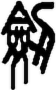
\includegraphics[width=0.8cm]{pictures/Schwert} }\\
Amonlonde im 8. Jahr d.G.d.R&\\
\end{tabular}
\vfill \vfill \vfill
Einst lud ein König in fernen Landen einen herausragenden Kämpfer an seinen
Hof, um ihn für seine Heldentaten zu ehren. Sie sprachen über ein
Schriftzeichen für das Wort \textit{Schwert}, in welchem der weise König eine
tiefere Bedeutung erkannt hatte. Er sagte zu dem Helden:
\begin{quote}\it
Der wahre Schwertkämpfer ist Eins geworden mit seiner Waffe. Die Klinge ist die
Verlängerung seiner Hand und er führt sie mit seinem Herzen.\\
Der Meister des Schwertes hingegen führt die Klinge am Gürtel und nimmt sie
nicht in die Hand. Sein Herz ist nun die Verlängerung der Waffe.\\
Doch Vollendung erreicht nur der, der die Klinge ganz aus seinem Herzen bannt.
\end{quote}
\newpage
\subsection*{Ad officii magistri}
Das Studium der Magie stellt sehr hohe Anforderungen an alle daran Beteiligten.
Die unbedarfte Anwendung eines Handwerks kann in kaum einem anderen Gebiet
derart großen Schaden anrichten. In den meisten Fällen gefährdet ein übermütiger Laie sich hauptsächlich selbst, wie beispielsweise in kämpferischen
Disziplinen, wird aber kaum seine Umgebung bedrohen. Anders in der Magie, wo
nur absolute Kontrolle der manipulierten Mächte die Realität in den Fugen
hält. 

Um diese Gefahr einzudämmen und trotzdem die Förderung von
Nachwuchsanwendern zu ermöglichen, ist eine Institutionalisierung der Ausbildung
nötig, welche klare Vorgaben über die Betreuung und Absicherung von ungelernten
Magiewirkenden macht. Die detaillierte Ausprägung einer solchen
\textit{Einrichtung} sei hier einmal dahingestellt.

Wichtig ist primär, dass zu jeder Zeit die Anforderungen, Kontrolle und
Anwendungsmöglichkeiten dem Wissensstand, der Befähigung und dem Potential
eines Novizen angepasst sind. Hierzu bedarf es der Supervision eines erfahrenen
Anwenders, eines Meisters beziehungsweise eines Magisters.
\newpage
\subsection*{Funktionen des Titels}
Der Titel des \meisters hat in diesem Zusammenhang vielfältige Funktionen.
\begin{itemize}
  \item Er weist auf einen bestimmten Reifegrad des Trägers hin.
  \item Er stellt ein Ziel dar, auf das der Novize seinen Ehrgeiz hin
  ausrichten kann, um die für sein Studium notwendige Disziplin zu erhalten.
  \item Er ist ein elementarer Schritt im Streben nach weiterer Weisheit
  eines jeden Magus.
  \item Er birgt weiterhin einen gesellschaftlichen Status und verleiht
  zusätzliche Rechte.
  \item Und er erlegt dem Träger eine Fülle von Pflichten und
  von Verantwortung gegenüber der Gesellschaft auf.
\end{itemize}

In dieser Arbeit soll hauptsächlich auf den letzten der genannten Punkte
eingegangen werden, weshalb die restlichen hier nur kurz beschrieben werden.

Der Titel \meister wird einem Anwärter von einer Entscheidungsinstanz
verliehen, welche die Tauglichkeit und die Erfüllung der notwendigen
Vorraussetzungen zuvor überprüft hat. Auf diese Weise wird sichergestellt, dass
jeder Träger dieses Titels die Erwartungen erfüllt, die man hernach an ihn
stellt.

Zu Beginn seiner Ausbildung hat der Novize selten eine Vorstellung davon,
welche Handlungsmöglichkeiten sich ihm im Laufe seiner weiteren Entwicklung
eröffnen und mit welchen Themengebieten er sich in Zukunft befassen kann. Daher
ist das endgültige Ziel zu dem er streben kann häufig all' zu abstrakt. Das
Erreichen des Meistergrades hingegen ist als Zwischenziel hervorragend
geeignet, da es der Novize sowohl als erreichbar wie aber auch als
herausfordernd wahrnimmt. Letztlich sollten sich höhere Ziele und das Interesse
an speziellen Themen der Kunst bis zum Erlangen des Meistergrades eingestellt
haben. Sie können sehr wohl auch als Kriterium zur Vergabe des Titels
herhalten.

Obwohl es keine explizite Regelung dazu gibt, zögert man nicht ohne Grund, einen
Lehrling bereits als \textit{Magus} zu bezeichnen. Die wirklich wichtige Arbeit auf
den Gebieten der Magie, die bahnbrechenden Entdeckungen und nachhaltigen
Entwicklungen sind dem Anwender fast ausschließlich erst dann möglich, wenn er
zumindest den Meistergrad erreicht hat. Die Entwicklung und Weiterentwicklung
seines Wesens als Magier kann ein Magieanwender nur betreiben, wenn er diesen
Schritt irgendwann in seiner Laufbahn tut. Ansonsten wird er immer ein Dilettant
bleiben. Diese Aussage ist allerdings insofern zu relativieren, als dass den
Meistergrad zu erreichen nicht unter allen Umständen bedeuten muss, von einem
Dritten den Titel verliehen zu bekommen.

So manch ein Magus findet sich in der Situation wieder, dass seine Bemühungen,
das Leben seiner Mitmenschen zu verbessern und seinen Beitrag zum Wohle der
Gemeinschaft zu leisten, nur fruchten können, wenn er profane
Entscheidungsträger auf bestimmte Erkenntnisse und Handlungsweisen aufmerksam
machen kann. Um der Tatsache Würdigung zu zollen, dass mit großer Macht auch
große Verantwortung für die Umwelt des Magieanwenders einher geht, werden einem
Meister gewisse Rechte innerhalb der Gesellschaft zugesprochen und er erhält
einen Status, der ihm auch von gesellschaftlich höhergestellten Personae
zumindest einen gewissen Respekt zusichern soll.

Als zentrale Elemente der Meisterschaft sind aber immer der neue Platz innerhalb
der magischen Gemeinschaft und die neuen Aufgaben und Verpflichtungen, die dem
Magus auferlegt werden zu betrachten:

\subsubsection*{Gehorsam}
Die Gehorsamspflicht gegenüber dem bisherigen Meister oder dem Institut, bei
dem die Verantwortung für die Ausbildung und den Novizen als solches lag,
erlischt, sofern sie nicht durch eine weiterführende Vereinbarung über eine
zukünftige Zusammenarbeit ersetzt wird.
Auch ein Meister hat nie ausgelernt und der Graduierte wäre töricht, nicht auch
weiterhin von der gängigerweise fortgeschrittenen Weisheit seines Ausbilders
weiterhin zu profitieren. 

Der unzweifelhafte Gehorsam gegenüber dem Ausbilder war während des Noviziats
das notwendige Gegenstück zu dessen persönlicher Verantwortlichkeit für das
Handeln seines Schützlings. Er wird im Rahmen einer kollegialen Kooperation, wie
sie oben erwähnt wird, durch eine Weisungsbefugnis der fortgeschrittenen Partei
über den Graduierten ersetzt.

\subsubsection*{Lehnstreue und ähnliche Verbindlichkeiten}
Hat der Graduierte einen \textit{weltlichen}, politischen, profanen oder
persönlichen Treueid geleistet, so bleibt dieser prinzipiell unangetastet. Er
wird nur insofern betroffen, als dass mit erreichen des Meistergrades dem Magus
eine größere Fülle von Handlungsmöglichkeiten zur Verfügung stehen, die er in
Erfüllung seiner Treuepflichten mit der dem Meister zugehörigen Sorgfalt zu
nutzen hat. 

Der Kern der Meisterschaft ist es, die Risiken der möglichen Applicationes zu
kennen, und all' solche als Handlungsmöglichkeit auszuschließen, welche
unvertretbare Risiken bergen. Um zu vermeiden, auf Geheiß eine solche
Applicatio ausführen zu müssen, sollte der Meister sie seinem Lehnsherrn nicht
als Alternative anbieten. Hier muss klar differenziert werden, wer die
Fachkenntnis besitzt, um solche Entscheidungen zu treffen auch wenn die
Befehlsgewalt woanders liegt.

Selbiges gilt natürlich auch für sämtliche anderen Vereinbarungen, die zu einer
Gehorsamspflicht oder -schuld gegenüber einer anderen Person führen.

\subsubsection*{Umgang mit Kollegae}
Der Graduierte ist nun ein vollwertiges Mitglied seiner Zunft. Mindestens
innerhalb seiner eigenen Magietradition ist er von den Kollegae als
gleichberechtigt zu behandeln. Es ist ihm gestattet, sich magischen
Gruppierungen (Zirkeln, Instituten usw.) als Mitglied oder Partner
anzuschließen oder solche zu gründen. Er erhält in der Regel Zugang zu
Schriften und sonstigen Ressourcen, welcher einem Novizen verwehrt würde.
Er hat das Recht, von gleichgestellten Kollegae und von Novizen den ihm
zustehenden Respekt einzufordern.

Selbstverständlich sind dem Meister Stellung und Respekt nur solange sicher,
wie sein Verhalten diesem Titel entspricht. Verantwortungsloses Handeln führt
selten zum Verlust des Meistergrades, aber sehr leicht zum Verlust von Respekt
und Vertrauen durch die Kollegae.

\subsection*{Forschung}
Der Magus ist mit erreichen des Meistergrades in der Lage und befugt,
selbstständig und eigenverantwortlich Forschung auf den Gebieten der Magie zu
betreiben oder sich an dieser zu beteiligen. Er ist angehalten, in regen
Austausch mit anderen Magi zu treten und seine Erkenntnisse in die Gemeinschaft
zurück zu tragen. 

Als Absolvent an einem akademischen Institut wird dem Forschenden häufig
umfangreiche Unterstützung zuteil. Darüber hinaus ist es aber auch üblich, dem
Institut die Ergebnisse der Arbeit abzutreten.

\subsubsection*{Lehre}
Die wohl wichtigste Pflicht des ausgebildeten Magieanwenders ist aber die Lehre
selbst. Grundsätzlich befindet sich ein Magus jederzeit in einer Lehrsituation,
ob als Lernender oder als Lehrender, zuweilen auch beides gleichzeitig. Nur
jemand, der dem Leben als Magus gänzlich entsagt, tritt aus diesem Kreislauf
aus. In diesem Falle ist er aber auch nicht mehr als Magiermeister in diesem
Sinne zu betrachten.

Zum einen darf der Meister niemals vergessen, sich weiterhin selbst der
Lehre zu unterziehen. Sei es durch das Studium bei anderen Meistern oder an
Instituten oder durch selbstständiges Erarbeiten und autodidaktische
Selbstschulung.

Zum anderen wurde ihm durch seine Ausbildung eine Gunst gewährt, welche er
durch sein Wirken zu begleichen hat. Allerdings wird diese Schuld nicht an
seinem Ausbilder getilgt, sondern an der magischen Gemeinschaft als solcher,
indem der Meister seinerseits das wissen um die Kunst an Novizen weitergibt.

Es ist dem Graduierten also auferlegt, das Wissen der Gemeinschaft zu mehren
und den Fortbestand seiner Lehren zu sichern. Dabei ist es seine Aufgabe, den
Zögling nach bestem Vermögen darauf vorzubereiten, selbst einmal die
Verantwortungen eines Magiermeisters zu bewältigen.

\subsubsection*{Meister des Schwertes}
Zum Abschluss soll nun Bezug auf die Einführung genommen werden. Dabei muss
wieder einmal das Schwert als bekanntester Vertreter der kriegerischen Künste als
Metapher für die Magie herhalten. 

Wie schon oft erlebt, wird die Benutzung und Beherrschung eines Schwertes gerne
und auch erfolgreich herangezogen, um einem profanen Gegenüber oder einem Laien
so manche Erkenntnis über die Magie zu vermitteln. Sei es, dass allein der
Anwender über die moralischen Implikationen der Anwendung entscheidet, oder
inwiefern es eher ein Werkzeug als eine Waffe darstellt. Diesem Beispiel folgend,
wird hier eine Weisheit über die Meisterschaft des Schwertes auf die
Meisterschaft der Magie übertragen.

Laut dem Ausspruch des weisen Königs versteht der Meister zweifellos, mit der
Waffe umzugenen, doch zeichnet er sich dadurch aus, die Klinge nicht zu ziehen.
Der lernende Magieanwender muss in allen Details wissen, wann er welche Formel
ausführen kann, um welchen Effekt zu erzielen. Ihm müssen sämtliche
Voraussetzungen und vor allem die Folgen klar sein, um jederzeit seine
Handlungsmöglichkeiten einschätzen zu können. Außerdem ist es unerlässlich, dass
er über diese theoretischen Fakten hinaus wohl geübt in der praktischen
Ausführung ist.

Als Meister sind seine Gedanken aber nicht auf die Möglichkeiten zu richten,
sondern auf die Notwendigkeiten. Neben einer Fehlerfreihen Beherrschung seiner
Formeln ist vor allen Dingen die ausschließlich sinnhafte Anwendung der Magie der
Ausdruck seiner Reife. 

Dies ist nur durch ausreichende Fachkenntnis zu erreichen, die auf einem
gefestigten Charakter fußt, der von klaren Verhaltensnormen geprägt ist. Hier sei
auf die Richtlinien der ulfaranistischen Moralvorstellung verwiesen.

Der Magiermeister trägt also die Magie in seinem Herzen, putzt seine Stiefel aber
trotzdem mit der Bürste.
\begin{figure}[h]
\raggedleft
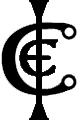
\includegraphics[width=0.3in]{pictures/Cordo_Siegel}
\end{figure}



\newpage

\chapter{Terminologie}

\begin{huge}
Lexikon der Magiohermetischen Terminologien
\end{huge}

\begin{small}

\begin{description}

  \item Abraxasgemme: aus der \textit{Alchemie}\
 \item Achat: edler Stein, Sinnbild für Emsigkeit und Fleiß, aber auch für Güte. Er vermag verwirrte Sinne zu heilen, aber auch Melancholie.\
 \item Adeptus: (A. minor, A. major) erster echter Titel eines Schülers, jemand, der die Lizenz erworben hat, seine Kunst frei zu lernen.\
 \item Aeromantie: Wahrsagen aus den Erscheinungen der \textit{Luft}, wie z.B. aus der Form der Wolken.\
 \item Aeternom: Sammelbegriff für Artefakte, die semipermanent oder permanent wirken.\
 \item Affinitäten (1): aus der Verschiedenheit der \textit{Elemente} ergibt sich bei Wahl eines einzelnen stets auch die 
 \item Entferntheit des Gegensätzlichen. Somit sind all die Beziehungen der Elemente untereinander, die Gegensätzlichkeiten und 
ihre Beiordnungen also ihre Affinitäten.\
 \item Affinitäten (2): dies sind bestimmte Materialien, welche von Dämonen begehrt oder verabscheut und welche also zur 
Beschwörung oder Vertreibung eines solchen verwendet werden. Die A. gehören zu der Gruppe der \textit{Paraphernalia}.
 \item Alchimie: Kunst und Wissenschaft zugleich, die sich mit der Veränderung der Materie vom Niederen zum Höheren befasst: 
unterteilt in die \textit{Niedere oder allgemeine Alchimie}, die auch des Öfteren mit der Kräuter- und Trankkunde gleichgesetzt wird, und zu deren Einsatz keine Zauberkunst nötig ist, und die \textit{}Hohe Alchimie, bei der dies sehr wohl der Fall ist.
 \item Allegorie: Gleichnis
 \item Alp: eine bösartige Geistererscheinung, die schwere Alpträume verursachen kann.
 \item Amethyst: edler Stein, er vermag ein Herz in flammende Leidenschaft zu versetzen. Sein Schimmer schenkt seinem Träger Schönheit und weckt Begehrlichkeiten.
 \item Analogien: Nach vielerlei Überlieferungen, vor allem alchimistischer Natur, soll es eine Reihe von Sympathien der Elemente mit Sternbildern, Planeten, Edelsteinen und dergleichen geben.
 \item Anatomie: die Kunde vom menschlichen Körper und seinen Funktionen.
 \item Antimagie: unter dem Begriffe der Antimagie oder Contra Magica versteht man all jene Zauberhandlungen, welchselbige zum 
Ziel haben, primo einen Zauber nicht zur Wirkung kommen zu lassen oder secundo eine bereits eingetretene Wirkung 
aufzuheben.
 \item Aquamarin: edler Stein, er symbolisiert die Kraft des Wassers und behütet den Seemann auf Fahrt. Er ist der Stein der Harmonie und Freundschaft.
 \item Archomagus, Archomaga: (auch Arcom.) Titel für Magier, der nur auf einem Konvent durch Beschluss der Gildenräte verliehen wird und die erfahrensten Magier ehren soll. Anrede: Euer Magnifizenz.
 \item Arkanogenese: Erschaffung eines magischen \textit{Artefakts}.
 \item Artefakt: hierbei handelt es sich um einen magischen Gegenstand, indem eine oder mehrere Zauber gespeichert sind und der auch von Nichtzauberern genutzt werden kann.
 \item Astralreise: das Loslösen des Astralleibes vom physischen Körper. 
 \item Astrolabium: feinmechanisches Rechenwerk. Zeigt für ein eingestelltes Datum den jeweiligen Stand der Sternbilder an.
 \item Astrologie: Die A. beschäftigt sich im Gegensatz zur \textit{Astronomie} mit der Deutung von Sternenkonstellationen und 
deren Einfluss auf die Geschicke der Sterblichen.
 \item Astronomie: die A. bezeichnet im Gegensatz zur \textit{Astrologie} die Sternkunde im Sinne der Erstellung und Erforschung 
von Sternkarten, insbesondere zur Navigation.
 \item Bann: dies ist die korrekte Anlage von Beschwörungs-Heptagramm, Schutzkreis sowie der Zeichen des zu beschwörenden Daimon, 
auch der Schutz- und Bannmächte als Teil der \textit{Paraphernalia}.
 \item Beherrschungsmagie: als Beherrschungsmagie oder Magica Contollaria kennen wir all jene Arten der Zauberei, welche in erster 
Linie auf den Geist des Opfers, will heißen, seinen Willen, sein Erinnern, gar auf seinen Instincto, nie jedoch auf seine 
Seele wirken.
 \item Bergkristall: edler Stein, Sinnbild der Erde. Er vermag Wunden zu heilen und den Körper zu stärken damit er schädlichen 
Einflüssen gewappnet ist.
 \item Bernstein: edler Stein, er ist das Symbol der Sonne und steht für den ersten Mond im Jahr. Sinnbild für Wahrhaftigkeit, 
Strenge und Gerechtigkeit.
 \item Beschwörungszauberei: Wir betrachten die B. oder Magica Conjuratio als Kunde von den Jenseitigen, allweil ähnliche Riten 
für \textit{Geister und \textit{Daimonen} Wirkung zeigen, so man sie in Persona invociren will. Item gehöret auch zur B. 
die Macht, Chimären und lebende Stand-Bilder zu machen, Pest und Siechtum zu conjuriren und letztendlich die finstere, 
lästerliche \textit{Necromantia} oder Untoten-Erhebung.
 \item Blutachat: \textit{Karneol}
 \item Blutmagie: „Mächtig aber ist das Blut, denn siehe! Es heilt die Kraft, so es von vornherein von Zaubertieren kommt, es gibt dir Kraft, so es nur von gemeinem Getier stammt. Am mächtigsten aber ist das Blut von Mensch und Elf. Um mit deinem Blute oder dem anderer zu zaubern, musst du einen eisernen Willen haben, denn es ist schiere Kraft am Werk, wo sonst Raffinesse und Kenntnis.
 \item Canton: allg. Zauberformel oder Spruch.
 \item Chimäre: mittels schwarzer Magie erzeugtes Mischwesen aus zwei oder mehr verschiedenen Tierarten, z.B. Harpyie, Greif oder Schlangenmensch.
Collega, Collegus: Anrede der Magier untereinander
 \item Conjuratio: Herbeirufung transsphärischer Wesenheiten. \textit{Beschwörungszauberei}
 \item Contramagie: \textit{Antimagie}
 \item Convocatus: Titulatur für die Mitglieder der Gildenräte. Anrede: Euer Spektabilität.
 \item Convocatus Primus: Sprecher der Gildenräte. Anrede: Euer Spektabilität.
 \item Daimon: jenseitiges Wesen, Bewohner der anderen Sphären: kann im Diesseits nur existieren, wenn er von einem Zauberkundigen 
beschworen wird. Man unterscheidet zwischen \textit{niederen Daimonen} und \textit{}höheren Daimonen}.
 \item Daimonologie: (Daimonologica) \textit{Beschwörungszauberei}
 \item Demonstratio: praktischer Teil der \textit{Examinatio}, bei dem der \textit{Adeptus minor} alle gelernten Sprüche, z.T. unter erschwerten Bedingungen demonstrieren muss.
 \item Diamant: edelster der Steine, Sinnbild für die Vollkommenheit und die arkane Kraft. 
 \item Diplomante: \textit{Magus}
 \item Disliberatio: mittelschwere Form der Bestrafung für Magier. Verbot der Benutzung aller Bibliotheken.
 \item Disputatio: theoretischer Teil der \textit{Examinatio}, bei dem die Kenntnisse bzgl. des weltlichen Wissens, der \textit{Alchimie}, der Rechtskunde und der klassischen Sprachen überprüft werden.
 \item Disvocatio: leichteste Form der Bestrafung für Magier. Ausschluss von allen höheren Ämtern wie der Akademieleitung oder der Mitgliedschaft im Gildenrat.
 \item Donaria: \textit{Paraphernalia}
 \item Donarium: so nennt man die Opfergabe eines bestimmten, seltsamen, dem \textit{Daimon} gefallenden Gegenstandes oder Tieres. Gehört zu den eventuellen
\textit{Paraphernalia} einer Beschwörung (\textit{Beschwörungs­zauberei}).
\item Dottore: \textit{Magister ordinarius}
 \item Drachen: allen Drachen gemein sind die schuppenbedeckte Haut, die geschlitzten Augen, die sie zur Nachtsicht befähigen, der meist sechsgliedrige Rumpf (von dem ein Beinpaar häufig zum Flügelpaar umgebildet ist) und der lange Schwanz. Es existieren verschiedenste Arten von Drachen ihnen allen eigen ist das man sie nur äußerst selten in den Mittellanden zu Gesicht bekommt. 
 \item Drow: eine den an Erscheinung den elfen ähnliche Rasse, mit dunkler Haut und meist weißen Haaren. Sie leben unter der Erde und haben einen unbändigen Hass auf alle anderen Lebenden Wesenheiten.
 \item Dschinn: \textit{Elemtharii}
 \item Dunkelelf: \textit{Drow}
 \item Ebene: \textit{Sphäre}
 \item Einhorn: vielerlei Namen hat das stolze Ross mit dem Horne: Einhorn nennt es die gemeine Bauernperson, Unicornu der Gelehrte, die Zwerge Ligorn und die Elfen Valdra. Es ist ein Ross mit schneeweißem Fell, langer weißer Mähne und einem ebensolchen Schweif. Auf der Stirn besitzt es ein güldenes, zwiefach gedrehtes Horn von fast drei Spann Länge. Auch Tiere mit silbernem Horn oder gar von nachtschwarzer Farbe mit einem Horn in der Farbe des Blutes sollen schon gesichtet worden sein.
 \item Elementarbeschwörung: die E. ist in der Tat eine \textit{Invocatio} und keine \textit{Conjuratio}, allweil die \textit{Elementharii} nicht jenseitig, sondern sehr
wohl unserer Sphäre zugeordnet sind.
 \item Elementare Transition: dies bezeichnet die Ver­schiebung eines Zaubers von einer elementaren Zu­ordnung in eine andere.
 \item Elementares Hexagramm: \textit{Siegel der Elemente}
 \item Elementargeist: \textit{Elementharii}
 \item Elementharii: eine beseelte Repräsentation elemen­tarer Kräfte.
 \item Elementarismus: \textit{Elementarbeschwörung} 
 \item Elemente: \textit{(Feuer, Wasser, Erde, Luft)}, die Elemente (auch: magische Elemente) sind die Bestandteile und Grundbausteine unserer Sphäre und alles Seins.
Ohne sie gäbe es keine Existenz und keine Substanz. 
 \item Eleve: \textit{Scolar}
 \item Erde: Erde und Natur. Hier findet sich alle belebte Materie wieder vom lebensspendenen Humus, über Käfer und Würmer, Kräuter und Bäume bis hin zu den großen Tieren 
und den kulturschaffenden Rassen, aber auch Holz und Leder, Knochen und welkes Laub. Kein Wunder also, dass die wichtigste Eigenschaft der Erde das Leben in all 
seinen Formen ist. (\textit{Elemente)}
 \item Erzmagier, \textit{Archomagus, Archomaga}
 \item Examinatio: Abschlussprüfung an einer magischen Akademie, bestehend aus \textit{Disputatio} und \textit{Demon­stratio}.
 \item Expurgico: schärfste Form der Bestrafung für Magier. Streichung aus der Akademieliste, Entfernung des Siegels, dadurch kein Schutz mehr durch das Gildenrecht.
 \item Fee: die wichtigsten der Arten sind die kleinen Blütenjungfern, auch Ladifari genannt, kaum spannen­groß in Blüten hausend, die Dryaden oder auch Nymphen, denen 
Pflanzen und Gewässer zu eigen sind, die greulichen Biestinger in aufrechter Tiergestalt, die Holden, von denen man spricht, sie seien die Vorfahren der Elfen, 
und die Wichtel und Kobolde, die wohl im Feenreiche als auf unsrer Seite der Tore zuhause sind.
 \item Feuer: Das Feuer steht nicht nur für das Herd- oder Lagerfeuer, sondern ist die Essenz von Wärme und Licht, Umwälzung und Vernichtung. Im wohnt eine große Kraft 
inne. (\textit{Elemente)}
 \item Gargyl: wenn dem Steine Leben eingehaucht wird, dass er ganz und gar einem Magus ergeben ist, so ist dies allemal wider die Natur und den Codex. Doch wisset von 
den Wasserspeiern, dass jener Magus, der sie ehedem erschuf, ihnen das Geheimnis des Lebens mit auf den Weg gab, ob zum Guten oder Bösen.
 \item Geister: gemeinhin die Seele eines Verstorbenen, der noch nicht ins Totenreich hinüber getreten ist.
 \item Geselle: Einteilung bei freien Lehrmeistern, gleiche Stufe wie ein \textit{Adept} an einer Akademie
 \item Ghul: diese menschenähnlichen Wesen besitzen eine graugrüne Haut, einen vorspringenden Kiefer mit gefährlichen Reißzähnen und lange Klauenhände. Um ihren 
Leichenschmaus abzuhalten, verlassen sie nur des Nachts ihre Gräber, denn das Licht der Sonne tötet sie.
 \item Gilde: Zusammenschluss mehrerer Akademien oder freier Magier
 \item Golem: ein aus Erde oder Stein bestehendes Wesen das durch magische weise zum Leben erweckt wurde.
 \item Greif: edles Wesen. Ein adlerköpfiger Löwe mit mächtigen Schwingen.
 \item Harpyie: nichts ist widernatürlicher als eine H. Halb Frau, halb Vogel und wirren Verstandes sind diese Ausgeburten der Schwarzen Magie. Harpyien kann man nie trauen, 
sie sind vollkommen unberechenbar.
 \item Heilmagie: Magie die auf den Körper wirkt um Wunden und Krankheiten zu heilen.
 \item Hermetica Destructiva: \textit{Kampfmagie}
 \item Hexalogien: Wenn es die elementare Manifestation einer Zauberwirkung gibt, wieso soll nicht auch für jedes \textit{Element} ein solcher Zauber existieren. Unter H. 
verstehen wir also, dass sich eine Zauberwirkung durch verschiedene Elemente erreichen lässt.
 \item Hippogriff: in entfernten Gebieten soll es Kreaturen geben, die aus der Brunft der Greifen entsprungen sind. Sie scheinen mit dem Pferd gekreuzt und bieten den 
Anblick einer Stute oder eines Hengstes mit dem Kopf, den Schwingen und den Fängen eines Adlers.
 \item Hohe Alchimie: Wissenschaft der Verwandlung von Materie. Im Gegensatz zur \textit{niederen Alchimie} oft unter Einsatz von Magie und komplexen Strukturen.
(\textit{Alchimie})
 \item Höhere Daimonen: eine Klasse von Wesen der anderen Sphären. Sie stehen in ihrer Macht deutlich über den \textit{Niederen Dämonen}.
 \item Hochmagier: \textit{Archomagus/a}
 \item Hofmagicus: Hofmagier (sowie meist Astrologe und Traum­deuter) eines Lehnsherren.
 \item Hypervehemenz: gleichzeitige Auslösung aller gestapelten Formeln zu einem Gesamteffekt.
 \item Irreversibilität: die Unwiderrufbarkeit einer Formel, also eines arkanen Musters, oder aber auch der Wirkung einer Formel, z.B. die I. der \textit{Antimagie}.
 \item Ingredenzien: Zutaten eines alchimistischen Rezeptes. (\textit{Alchimie})
 \item Invocatio: Herbeirufung (normalerweise eines Elementes: auch \textit{Dschinne} etc.)
 \item Invocatio Daimoniae: \textit{Beschwörungszauberei}
 \item Invocatio Elementharii: \textit{Elementarbeschwörung}
 \item Kadunom: Sammelbegriff für alle Artefakte, die auf Ladungen basieren.
 \item Kampfmagie: Magie die zur Unterstützung im Kampfe oder zum direkten Schaden eines Feindes eingesetzt wird. Einteilung erfolgt meist nach Ziel des Zaubers und 
nicht nach der direkten Wirkung.
 \item Karneol: edler Stein, er ist das Sinn­bild für Ruhe, Vergessen, innere Kraft, aber auch für das unwiderrufliche Ende. Er spendet den Trauernden Trost, den Rastlosen
Ruhe, dem Zornigen Frieden.
 \item Kender: kleine Geschöpfe mit meist kindlichem Gemüte, empfinden keine Angst und finden oft Dinge die ihnen nicht gehören.
 \item Klabautermann: besondere \textit{Kobolde} sind die K., die ein wahrlich uraltes Gesicht auf einem Kindskörper zur Schau tragen. Man findet sie häufig auf alten 
Schiffen, denn sie sind der fleischgewordene Geist eines solchen Fahrzeugs oder des Holzes, aus dem es gebaut wurde.
 \item Kobold: gar sonderlich anzuschauen sind die Kobolde, welche die Menschen allzu gerne durch ihre Schelmereien plagen. Sie besitzen die Gabe der Zauberei und sind 
nach menschlichen Ansätzen oft von sehr seltsamem Wesen. Man sagt, dass ein Mensch Macht über einen K. gewinnt, wenn er seinen Namen kennt und ruft.
 \item Komponenten: Zutaten und Gegenstände die für eine Zauberhandlung notwendig sind.
 \item Lapislazuli: edler Stein, in ihm findet sich die Kraft der Luft. Er ist der Schutzstein der Wanderer und Abenteurer. Er weist dem Reisenden den Weg und vermag 
durch seine Kraft, Unglücksfälle zu verhüten.
 \item Lehrling: Einteilung bei freien Lehrmeistern, gleiche Stufe wie ein \textit{Scolar an einer Akademie}.
 \item Licenzore: \textit{Adeptus}
 \item Luft: Wind und Sturm. Dies ist nicht nur die Luft, die wir atmen, es ist auch der Wind, vom lauen Lüftchen bis hin zum entfesselten Sturm. Demzufolge sind mit der 
Luft auch Eigenschaften wie Bewegung und Flüchtigkeit verbunden. (\textit{Elemente})
 \item Lykanthropie: \textit{Werkreatur}
 \item Magia Anime: \textit{Beherrschungsmagie}
 \item Magia Galad: \textit{Kampfmagie}
 \item Magia Medicam: \textit{Heilmagie}
 \item Magia Sanctum: \textit{Schutzmagie}
 \item Magica Combativa: \textit{Kampfmagie}
 \item Magica Conjuratio: \textit{Beschwörungszauberei}
 \item Magica Contraria: \textit{Antimagie}
 \item Magica Controllaria: \textit{Beherrschungsmagie}
 \item Magica Transformatorica: \textit{Verwandlungsmagie}
 \item Magiergilde: \textit{Gilde}
 \item Magister, Magistra: Titel nach erfolgreicher Meisterprüfung.
 \item Magister magnus: M. m. dürfen sich all jene nennen, die entweder als Lehrstuhlinhaber an Akademien oder als freie Meister das Recht haben, Eleven und 
\textit{Scolaren} anzunehmen und ein eigenes Siegel zu führen.
Magister spectabilitas: Akademieleiter.
 \item Magnifizenz: Anrede für einen \textit{Erzmagier}.
Magus, Magica: Die Bezeichnung für alle Gelehrten, die ihre \textit{Examinatio} bestanden, und die Lizenz erworben haben, ihre Wissenschaft zu praktizieren. Anrede:
gelehrte/r Dame/­Herr
 \item Magister extraordinarius: freier Lehrer oder nicht ständiger Lehrer einer Akademie.
 \item Magister ordinarius, Magia ordinaria: (Akademie-) Lehrer bzw. Lehrerin, bisweilen auch Titel eines an­erkan­nten Großmeisters.
 \item maiestro de thesis...: Meister der Thesis.....
 \item Matrix: Gitter oder Netz, welches als Medium für eine Spruch­wirkung dient. Matrices werden unterteilt in M. naturalis (nat., solche die natürlich in der Welt existieren und recht unstrukuriert sind), M. artificialis (art., von Zauberkundigen selbst erschaffene M.) und M. arcana (arc., sehr komplexe in hochmagischen Körpern vor­kommende M.)
 \item Metamagie: zur M. gehören jene Formeln, welche ver­ändernd auf Matrices artificialis und arcana wirkt: \textit{Matrix}.
 \item Metaphorische Transition: dies bezeichnet die Ver­schiebung eines Zaubers von einem Spezialgebiet in ein anderes.
 \item monophil: Eigenschaft eines Artefakts, das nur von einem einzigen Träger üblicherweise dem Erschaffer - angewendet werden kann.
 \item Nachtalp: \textit{Alp}
 \item Nanduria: (auch: Nandus-Schrift) die 26 Zeichen des Nanduria werden bei Magiern, Alchimisten und einige anderen Gelehrten zur Aufzeichnung von Geheimnissen benutzt, aber auch bei Gravuren oder der Herstellung magischer \textit{}Artefakte finden sie Anwendung.
 \item Necromantia: (Nekromantie) die N. ist die Lehre von den \textit{Untoten}. Sie befasst sich mit der gar ­lästerlichen Erweckung, aber auch mit der Beherrschung derselben. Die N. gilt allgemein als ver­abscheuungs­würdigste Form der Zauberei und ihre Aus­übung steht wohl vielerorts unter harter Strafe.
 \item Necropathia: dies ist die Ver­ständigung mit den Verstorbenen, welche auf magische Weise geschieht.
 \item Niedere Alchimie: (manchmal auch Trankkunde), die n. A. beschreibt im Gegensatz zur \textit{Hohen Alchimie} die Herstellung von einfachen Rezepten und Tränken die meist auf der direkten Wirkung ihrer Ingredenzien basieren. (\textit{}Alchimie)
 \item Niedere Daimonen: unterste Klasse der \textit{Daimonen}. 
 \item Novize: \textit{Scolar}
 \item Obsekrator: Artefakt, dessen Auslösung eine \textit{Beschwörung} bewirkt.
 \item Okkupation: Beseeltheit eines Artefakts: astrale/­elementare/­­transnekrotische/­daimonische Okkupation.
 \item Onyx: edler Stein, er hat Macht über \textit{Daimonen} und \textit{Geister} und über die Gefilde, in denen die Toten wandeln. Er vermag den Kundigen sicher durch die verschlungenen Pfade der astralen Sphäre zu geleiten und bewahrt ihn davor, darin verloren zu gehen.
 \item Opal: edler Stein, in ihm zeigen sich alle Farben, er ist das Sinnbild der Vielfalt. Er hat die Macht die Jugend zurückzugeben.
 \item Paraphernalia: so werden die Randbedingungen ge­nannt, welche es bei Beschwörungen von \textit{Daimonen} zu beachten gilt. Dazu gehören einmal das \textit{}Temporalium, der Bann, die \textit{}Affinitäten sowie unter Um­ständen das \textit{}Donarium. (\textit{}Beschwörungszauberei)
 \item Präservanz: Wirkungszeitraum der gespeicherten Sprüche: einmalig, aufladbar, semipermanent, permanent.
 \item Parenthese: Nebeneffekt, der nicht durch die wirkenden Sprüche bewirkt wird.
 \item Poltergeist: Erscheinungsform eines \textit{Geistes}, meist an einen bestimmten Ort gebunden.
 \item Quarz: \textit{Bergkristall}
 \item Rattenmenschen: \textit{Skaven}
 \item Rehermetifikation: Wiederaufladung, Wideraufladbarkeit eines Artefaktes.
 \item Rettore, Rettrice: \textit{Magister spectabilitas}
 \item Rubin: edler Stein, in ihm findet sich die Kraft des Feuers. Mit ihm kann man die Flammen beherrschen, er kann aber auch den lodernden Zorn in der Brust eines Kriegers wecken.
 \item Runenschrift: meist alte Schrift die verschiedene Zeichen nutzt. Es existieren viele verschiedene Formen von Runenschriften.
 \item Saphir: edler Stein, das Sinnbild der Rein­heit und Beständigkeit, der Stein der Liebenden, die zueinander gefunden haben. In ihm liegt die Kraft des Seelenfriedens und der Freundschaft.
 \item Satyr: Wesenheit mit menschlichem Körper aber den Beinen einer Ziege.
 \item Scolar: (auch: Eleve, Novize, Studiosi, Lehrling) Bezeichnung für einen Schüler einer Magierakademie oder eines freien Lehr­meisters, je nach Wissensstand. 
 \item Siegel der Elemente: nach dem „\textit{Groszen Elemen­tharium} stellt dieses die allgemein gültigen Gesetze und Gegensätze der Elemente dar. (\textit{}Elementarbeschwörung)
 \item Skaven: kleine einer Ratte ähnliche Geschöpfe die tief in der Erde hausen. Sie nutzen oft die Kraft magischer Steine, allen voran den seltsamen \textit{}Wechselstein. 
 \item Smaragd: edler Stein, er steht für Mut, Hoffnung und Treue. Mit ihm beschwört man das Schlachtenglück. Unter seinem Schimmer wird der Feigling zum Helden, der Held aber erfährt ungeahnten Mut.
 \item Sphäre: alle Ebenen jenseits der unsrigen.
 \item Spektabilität (1): Anrede für einen \textit{Convocatus}.
 \item Spektabilität (2): \textit{Magister spectabilitas}
 \item Sternkunde: \textit{Astrologie},\textit{Astronomie}
 \item Spezialgebiet: allgemein gültige, auf dem „Groszen Arcanum beruhende Einteilung der verschiedenen Bereiche der Zauberei nach ihrem Ziel und Zweck, nicht aber nach den Modalitäten des Zaubervorgangs. Ein S. der Magie, der ein Spruch zuzurechnen ist, z.B. Kampf.
 \item Schutzmagie: Magie die zum Schutze der eigenen oder anderer Personen genutzt wird
 \item Studiosi: \textit{Scolar}
 \item Technik (eines Zaubers): dies sind die Zauber­hand­lungen, die vom Magiekundigen auszuführen sind, sei dies das laute Rezitieren einer Formel oder eine Hand­bewegung.
 \item Temporalium: dies sind die Umstände der Be­schwörung, welche seien die korrekte Tageszeit, der kor­rekte Ort und besondere Sternkonstellationen. Diese müs­sen natürlich mit den restlichen \textit{}Para­phernalia der Be­schwörung übereinstimmen. (\textit{}Beschwörungs­zauberei)
 \item Thesis: dies ist die Summe von komplexen geo­metrischen Mustern, den Kraftfäden der \textit{}Matrix, welche die Eigenschaften eines Zaubers und die Zauberformel beinhalten.
 \item Thaumaturgie: Artefaktzauberei, eigentlich alle Aus­formungen der Hohen Magie, im Gegensatz zur Profan­magie der Scharlatane und Naturzauberkundigen.
 \item Thaumatursom: Träger der Verzauberungssprüche: das Artefakt, bisweilen auch Sammelbezeichnung für \textit{}Aeternome und \textit{}Kadunome.
 \item Trankkunde: \textit{niedere Alchimie}
 \item Transmutatio: eine größere Freveltat noch als die Be­lebung von Toten zu Untoten ist das Erschaffen völlig künstlichen Lebens Transmutatio welches allen gött­lichen und natürlichen Gesetzen widerspricht und daher nur mittels \textit{}Beschwörungszauberei zu voll­bringen ist.
 \item transsphärische Wesenheiten: Bewohner der äußeren \textit{Sphären}.
 \item Türkis: edler Stein, er ist zugleich Glücks­bringer und Sinnbild für Unbeständigkeit. Er lässt Herzenswünsche wahr werden. Er ist der Freund des Spielers, verleiht den Händen magische Flinkheit.
 \item ultima occasio: günstigste Vorgaben zur Artefakt­erschaffung.
 \item Unicornu: \textit{Einhorn}
 \item Untote: von den wandernden Toten: Alle Nicht-Toten sind gar schauerlich anzusehen und von üblem Geruch umgeben. Wer sie berührt, den rafft die Pest dahin. Nicht-Tote sind unheilig, denn ihr Dasein ist ein Frevel.
 \item Vampir: Vampire haben spitze Zähne und beißen ihre Opfer in den Hals um ihr Blut zu trinken. Viele können sich in Fledermaus und Wolf verwandeln, sowie selbige herbeirufen. Sie hassen Knoblauch, heilige Symbole und geweihtes Wasser. Sie fürchten sich vor dem hellen Lichte der Sonne. Werden sie bezwungen, fliehen sie an einen dunklen Ort, oft in ihren Sarg. Getötet werden sie mit einem Holzpflock von Weißdorn oder Eiche, welchen man ihnen direkt ins Herz treiben muss.
 \item Verwandlungsmagie: Magie die einen direkten Einfluss auf Form, Substanz oder andere stoffliche Eigenschaften eines Objektes hat.
 \item Waldmännchen: \textit{Kobold}
 \item Wasser: Feuchtigkeit und Flüssigkeit. Im Wasser finden nicht nur Tiefe und Unergründlichkeit ihre Re­präsen­tation, sondern vor allem die Veränderlichkeit und die Kraft der langsamen, aber stetigen Veränderung. Unergründlicher Geist und auch Melancholie und Wahn­sinn werden mit dem Wasser assoziiert, ebenso wie Wandelbarkeit, Beweglichkeit und Eleganz. (\textit{}Elemente)
 \item Wasserspeier: \textit{Gargyl}
 \item Wechselstein: seltsamer Stein, mit unbekannter magischer Kraft. Wird oft von \textit{Skaven} für allerlei schreckliche Dinge genutzt.
 \item Werkreatur: Fluch und Krankheit gleichermaßen ist die Lykanthropie, die Menschen in wilde Tiere ver­wandelt: Die Werwesen. Wenn der Mond voll ist, bricht das Wertier hervor. Manche Opfer werden gänzlich zum Tier, andere verwandeln sich in ein Mischwesen. Nicht Gewalt noch Vernunft können sie halten, ihre Blutgier ist größer als die jeder Kreatur, und nichts kann sie erlösen als eine Klinge von purem Silber.
 \item Widergänger: \textit{Untote}
 \item Xenophon: unbekannter wirkender Spruch.
 \item Zhayad: eine besonders bei Beschwörern (\textit{Be­schwörungs­zauberei}) beliebte Geheimsprache und Schrift, von der behauptet wird nur in ihr könne man die 
korrekten Formeln sprechen. 
 \item Zombie: \textit{Untote}

\end{description}

\end{small}

Thalian Sanderfels, überarbeitete Version, 12. Februare 1004

\appendix



\chapter{"uber den Autor}

%\yinipar{F}
Florian Phelleas Ph"onixflug wurde im Jahre 232 nach Jeldrik auf Burg Hanekamp in Engonien gebohren. Durch seinen Vater Aldus, Haushofmagier des Herzogs von Hanekamp 
und seine Mutter Anastasia seit fr"uhester Kindheit gef"ordert schlug er schon in jungen Jahren eine hervorragende akademische Karriere ein.
Mit zw"olf Jahren wurde er von Magus Galad et Sanctum Cederic Greifenhorst, als Lehrling angenommen und trat nach Gr"undung des Bundes zu Ayd Owl durch seinen Meister, 
dem Bund als einer der ersten Sch"uler bei. Im Alter von 16 Jahren wurde er Lehrling des Bundes zu Ayd Owl und im Alter von 18 Jahren zum Scolarius.
Als Scolarius absolvierte er Gaststudien an der Akademie zu Amonlonde und der Cantus Harmonae zu Condra. Ferner belegte er bereits w"ahrend dieser Lehrzeit den zweiten 
Platz im offenen Ritualkontest der Akademie zu Montralur.\
Im Alter von 23 Jahren trat er in die Dienste des Markgrafen Jerevan zu Arkenwald aus Grenzbrueck und wurde von der Akademia zu Ayd Owl in den Adeptenstatus erhoben. 
In den Diensten des Markgrafen erhielt er einen Lehrauftrag f"ur die Ars Bellorum von Arkenwald.\
Mit 25 Jahren trat er der Akadmia Clavis Mundi Grenzbrueckensis im Range eines Adepten bei und begann weiterf"uhrende Forschungen auf dem Gebiet der Ars Magica Temporalis.
Mit 26 Jahren promovierte er mit seiner Arbeit "uber Deterministisches Schicksal und Chaos an der Akademia Clavis Mundi als Magus Minor.
Das folgende Jahr lehrte und forschte er als Assistent von Senator, Magus Galad et Contra, Praeceptor Primus Galadmagica Erszbet Lauschenberg im Bereich der Galadmagica 
und der Ars Magica Temporalis an der Akademia Clavis Mundi Grenzbrueckensis, bis er zum persönlichen Assistenten der Akademieleitung berufen wurde. In dieser Funktion
übernahm er auch das administrative Amt der Licensiatur und habilitierte mit 27 in der Galadmagia mit seinen Vorlesungen zur Pyrodynamik. 
Im Frühsommer des Jahres 260 nach Jeldrik heirate er Lix von der Academia Cantus Harmonae.\
Als in Folge des
grenzbruecker Reychstages von 1401 die Akademia Clavis Mundi unter Hausarrest gestellt und einer Untersuchung unterzogen wurde, verweigerte er die Unterstellung der Akademie
und seiner Person unter das weltliche Recht der grenzbruecker Krone und wurde infolgedessen zum Reichsverräter erklärt.\
Nach der Flucht aus Grenzbrueck lebt er zur Zeit mit seiner Ehefrau, seinem Neffen und seiner Nichte in Tharemis, der Hauptstadt des freien Condra, führt private Studien
im Spezialgebiet der metaphysischen Elementarlehre durch und protegiert einzelne, ausgewählte Schüler der Academia Cantus Harmonae.





\end{document}

